\documentclass[12pt]{article} 
\usepackage[margin=2cm]{geometry} 
\usepackage{psfrag} 
\usepackage{graphicx} 
\usepackage{epstopdf} 
\usepackage{longtable,booktabs} 
\usepackage{amsmath,amsfonts} 
\usepackage{breqn} 
\usepackage{float,morefloats,caption} 
\begin{document} 
% 23-Jan-2024 16:35:14, created by McMCDiagnostics.m 
 
\begin{center}
\begin{longtable}{lcc} 
\caption{MCMC Inefficiency factors per block}\\
 \label{Table:MCMC_inefficiency_factors}\\
\toprule 
$Parameter          $	 & 	 $     Block~1$	 & 	 $     Block~2$\\
\midrule \endfirsthead 
\caption{(continued)}\\
 \toprule \\ 
$Parameter          $	 & 	 $     Block~1$	 & 	 $     Block~2$\\
\midrule \endhead 
\midrule \multicolumn{3}{r}{(Continued on next page)} \\ \bottomrule \endfoot 
\bottomrule \endlastfoot 
$ \sigma_{{e_ZI}}   $	 & 	     488.250	 & 	     464.099 \\ 
$ \sigma_{{e_Z}}    $	 & 	     613.961	 & 	     580.273 \\ 
$ \sigma_{{e_N}}    $	 & 	     548.772	 & 	     550.104 \\ 
$ \sigma_{{e_D}}    $	 & 	     290.988	 & 	     221.325 \\ 
$ {\rho_Z}          $	 & 	      92.013	 & 	      80.247 \\ 
$ {\rho_ZI}         $	 & 	     732.176	 & 	     708.002 \\ 
$ {\rho_N}          $	 & 	     512.506	 & 	     472.244 \\ 
$ {\rho_D}          $	 & 	     447.667	 & 	     435.102 \\ 
\end{longtable}
 \end{center}
% End of TeX file.
 
% 21-Jan-2024 18:59:42, created by stoch_simul.m 
 
\begin{center}
\begin{longtable}{lcccc} 
\caption{MATRIX OF COVARIANCE OF EXOGENOUS SHOCKS}\\
 \label{Table:covar_ex_shocks}\\
\toprule 
$Variables  $	 & 	 $       {e_Z}$	 & 	 $      {e_ZI}$	 & 	 $       {e_N}$	 & 	 $       {e_D}$\\
\midrule \endfirsthead 
\caption{(continued)}\\
 \toprule \\ 
$Variables  $	 & 	 $       {e_Z}$	 & 	 $      {e_ZI}$	 & 	 $       {e_N}$	 & 	 $       {e_D}$\\
\midrule \endhead 
\midrule \multicolumn{5}{r}{(Continued on next page)} \\ \bottomrule \endfoot 
\bottomrule \endlastfoot 
${e_Z}      $	 & 	    0.000056	 & 	    0.000000	 & 	    0.000000	 & 	    0.000000 \\ 
${e_ZI}     $	 & 	    0.000000	 & 	    0.000603	 & 	    0.000000	 & 	    0.000000 \\ 
${e_N}      $	 & 	    0.000000	 & 	    0.000000	 & 	    0.000421	 & 	    0.000000 \\ 
${e_D}      $	 & 	    0.000000	 & 	    0.000000	 & 	    0.000000	 & 	    0.038138 \\ 
\end{longtable}
 \end{center}
% End of TeX file.
 
% 23-Jan-2024 16:36:11, created by compute_moments_varendo.m 
 
\begin{center}
\begin{longtable}{lcccc} 
\caption{Posterior mean variance decomposition (in percent)}\\
 \label{Table:dsge_post_mean_var_decomp_uncond}\\
\toprule 
$                $	 & 	 $     {e_Z}$	 & 	 $    {e_ZI}$	 & 	 $     {e_N}$	 & 	 $     {e_D}$\\
\midrule \endfirsthead 
\caption{(continued)}\\
 \toprule \\ 
$                $	 & 	 $     {e_Z}$	 & 	 $    {e_ZI}$	 & 	 $     {e_N}$	 & 	 $     {e_D}$\\
\midrule \endhead 
\midrule \multicolumn{5}{r}{(Continued on next page)} \\ \bottomrule \endfoot 
\bottomrule \endlastfoot 
$I\_obs          $	 & 	     98.52	 & 	      0.89	 & 	      0.15	 & 	      0.43 \\ 
$C\_obs          $	 & 	     99.76	 & 	      0.11	 & 	      0.06	 & 	      0.06 \\ 
$Y\_obs          $	 & 	     99.79	 & 	      0.03	 & 	      0.07	 & 	      0.11 \\ 
$lab\_prod\_obs  $	 & 	     99.79	 & 	      0.04	 & 	      0.08	 & 	      0.09 \\ 
$p\_I\_obs       $	 & 	     99.45	 & 	      0.51	 & 	      0.01	 & 	      0.03 \\ 
$log\_D          $	 & 	     81.66	 & 	      0.02	 & 	      0.07	 & 	     18.26 \\ 
$log\_N          $	 & 	     98.59	 & 	      0.02	 & 	      1.25	 & 	      0.14 \\ 
\end{longtable}
 \end{center}
% End of TeX file.
 
\begin{center}
\begin{longtable}{ccc}
\caption{Endogenous}\\%
\hline%
\multicolumn{1}{c}{\textbf{Variable}} &
\multicolumn{1}{c}{\textbf{\LaTeX}} &
\multicolumn{1}{c}{\textbf{Description}}\\%
\hline\hline%
\endfirsthead
\multicolumn{3}{c}{{\tablename} \thetable{} -- Continued}\\%
\hline%
\multicolumn{1}{c}{\textbf{Variable}} &
\multicolumn{1}{c}{\textbf{\LaTeX}} &
\multicolumn{1}{c}{\textbf{Description}}\\%
\hline\hline%
\endhead
\texttt{Y} & ${Y}$ & output\\
\texttt{C} & ${C}$ & consumption\\
\texttt{I} & ${I}$ & investment\\
\texttt{K} & ${K}$ & Capital\\
\texttt{K\_C} & ${K_C}$ & Capital:C\\
\texttt{K\_I} & ${K_I}$ & Capital:I\\
\texttt{N} & ${N}$ & Hours\\
\texttt{N\_C} & ${N_C}$ & Hours:C\\
\texttt{N\_I} & ${N_I}$ & Hours:I\\
\texttt{Z\_C} & ${Z_C}$ & Tech:C\\
\texttt{u\_ZI} & $u\_ZI$ & u\_ZI\\
\texttt{Z\_I} & ${Z_I}$ & Tech:I\\
\texttt{theta\_N} & ${\theta_N}$ & Labor disutility\\
\texttt{theta\_D} & ${\theta_D}$ & Shopping disutility\\
\texttt{R\_C} & ${R_C}$ & Capital rental rate:C\\
\texttt{R\_I} & ${R_I}$ & Capital rental rate:I\\
\texttt{W} & ${W}$ & Real wage\\
\texttt{D} & ${D}$ & Shopping effort\\
\texttt{D\_C} & ${D}$ & Shopping effort:C\\
\texttt{D\_I} & ${D}$ & Shopping effort:I\\
\texttt{Gam} & ${\Gamma}$ & Composite utility term\\
\texttt{p\_I} & ${p_I}$ & Relative investment price\\
\texttt{log\_Y} & $log\_Y$ & log\_Y\\
\texttt{log\_C} & $log\_C$ & log\_C\\
\texttt{log\_I} & $log\_I$ & log\_I\\
\texttt{log\_N} & $log\_N$ & log\_N\\
\texttt{log\_Y\_N} & $log\_Y\_N$ & log\_Y\_N\\
\texttt{log\_D} & $log\_D$ & log\_D\\
\texttt{C\_obs} & $C\_obs$ & C\_obs\\
\texttt{I\_obs} & $I\_obs$ & I\_obs\\
\texttt{Y\_obs} & $Y\_obs$ & Y\_obs\\
\texttt{lab\_prod\_obs} & $lab\_prod\_obs$ & lab\_prod\_obs\\
\texttt{p\_I\_obs} & $p\_I\_obs$ & p\_I\_obs\\
\hline%
\end{longtable}
\end{center}
\begin{center}
\begin{longtable}{ccc}
\caption{Exogenous}\\%
\hline%
\multicolumn{1}{c}{\textbf{Variable}} &
\multicolumn{1}{c}{\textbf{\LaTeX}} &
\multicolumn{1}{c}{\textbf{Description}}\\%
\hline\hline%
\endfirsthead
\multicolumn{3}{c}{{\tablename} \thetable{} -- Continued}\\%
\hline%
\multicolumn{1}{c}{\textbf{Variable}} &
\multicolumn{1}{c}{\textbf{\LaTeX}} &
\multicolumn{1}{c}{\textbf{Description}}\\%
\hline\hline%
\endhead
\texttt{e\_Z} & ${e_Z}$ & TFP shock\\
\texttt{e\_ZI} & ${e_ZI}$ & Investment-specific tech shock\\
\texttt{e\_N} & ${e_N}$ & Labor supply shock\\
\texttt{e\_D} & ${e_D}$ & Shopping disutility shock\\
\hline%
\end{longtable}
\end{center}
\begin{center}
\begin{longtable}{ccc}
\caption{Parameters}\\%
\hline%
\multicolumn{1}{c}{\textbf{Variable}} &
\multicolumn{1}{c}{\textbf{\LaTeX}} &
\multicolumn{1}{c}{\textbf{Description}}\\%
\hline\hline%
\endfirsthead
\multicolumn{3}{c}{{\tablename} \thetable{} -- Continued}\\%
\hline%
\multicolumn{1}{c}{\textbf{Variable}} &
\multicolumn{1}{c}{\textbf{\LaTeX}} &
\multicolumn{1}{c}{\textbf{Description}}\\%
\hline\hline%
\endhead
\texttt{gam} & ${\gamma}$ & Risk aversion\\
\texttt{r\_ann} & ${r_ann}$ & Annual interest rate\\
\texttt{g\_bar} & ${\overline{g}}$ & Quarterly growth rate\\
\texttt{nu} & $(\nu)$ & Frisch elasticity\\
\texttt{I\_Y} & $(I_Y)$ & Investment-output ratio\\
\texttt{K\_Y} & $(K_Y)$ & Capital-output ratio (quarterly)\\
\texttt{labor\_share} & $(labor share)$ & Labor share\\
\texttt{phi} & $(\phi)$ & Shopping matching function elasticity\\
\texttt{eta} & $(\eta)$ & Shopping disutility\\
\texttt{Psi} & $(\Psi)$ & Matching utilization\\
\texttt{rho\_Z} & ${\rho_Z}$ & persistence TFP shock\\
\texttt{rho\_ZI} & ${\rho_ZI}$ & persistence I-specific shock\\
\texttt{rho\_N} & ${\rho_N}$ & persistence labor supply shock\\
\texttt{rho\_D} & ${\rho_D}$ & persistence shopping effort shock\\
\texttt{p\_I\_ss} & $p\_I\_ss$ & p\_I\_ss\\
\texttt{N\_ss} & $N\_ss$ & N\_ss\\
\hline%
\end{longtable}
\end{center}
 
\begin{center}
\begin{longtable}{ccc}
\caption{Parameter Values}\\%
\toprule%
\multicolumn{1}{c}{\textbf{Parameter}} &
\multicolumn{1}{c}{\textbf{Value}} &
 \multicolumn{1}{c}{\textbf{Description}}\\%
\midrule%
\endfirsthead
\multicolumn{3}{c}{{\tablename} \thetable{} -- Continued}\\%
\midrule%
\multicolumn{1}{c}{\textbf{Parameter}} &
\multicolumn{1}{c}{\textbf{Value}} &
  \multicolumn{1}{c}{\textbf{Description}}\\%
\midrule%
\endhead
${\gamma}$ 	 & 	 1.000 	 & 	 Risk aversion\\
${r_ann}$ 	 & 	 0.040 	 & 	 Annual interest rate\\
${\overline{g}}$ 	 & 	 0.000 	 & 	 Quarterly growth rate\\
$(\nu)$ 	 & 	 0.720 	 & 	 Frisch elasticity\\
$(I_Y)$ 	 & 	 0.200 	 & 	 Investment-output ratio\\
$(K_Y)$ 	 & 	 11.000 	 & 	 Capital-output ratio (quarterly)\\
$(labor share)$ 	 & 	 0.670 	 & 	 Labor share\\
$(\phi)$ 	 & 	 0.320 	 & 	 Shopping matching function elasticity\\
$(\eta)$ 	 & 	 0.200 	 & 	 Shopping disutility\\
$(\Psi)$ 	 & 	 0.810 	 & 	 Matching utilization\\
${\rho_Z}$ 	 & 	 0.999 	 & 	 persistence TFP shock\\
${\rho_ZI}$ 	 & 	 0.733 	 & 	 persistence I-specific shock\\
${\rho_N}$ 	 & 	 0.944 	 & 	 persistence labor supply shock\\
${\rho_D}$ 	 & 	 0.825 	 & 	 persistence shopping effort shock\\
$p\_I\_ss$ 	 & 	 1.000 	 & 	 p\_I\_ss\\
$N\_ss$ 	 & 	 0.300 	 & 	 N\_ss\\
\bottomrule%
\end{longtable}
\end{center}
 
% TeX-table generated by Dynare write_latex_prior_table.m.
% Prior Information
% 23-Jan-2024 16:36:12 
 
\begin{center}
\begin{longtable}{lcccccccc} 
\caption{Prior information (parameters)}\\
 \label{Table:Prior}\\
\toprule%
  &  &  &  &  & \multicolumn{2}{c}{Bounds} & \multicolumn{2}{c}{90\% HPDI} \\ 
  \cmidrule(r{.75em}){6-7} \cmidrule(r{.75em}){8-9}
  & Distribution & Mean & Mode & Std.dev. & Lower & Upper & Lower & Upper  \\ 
\midrule
\endfirsthead
\caption{(continued)}\\
 \toprule%
  &  &  &  &  & \multicolumn{2}{c}{Bounds} & \multicolumn{2}{c}{90\% HPDI} \\ 
  \cmidrule(r{.75em}){6-7} \cmidrule(r{.75em}){8-9}
  & Distribution & Mean & Mode & Std.dev. & Lower & Upper & Lower & Upper  \\ 
\midrule
\endhead
\midrule
\multicolumn{9}{r}{(Continued on next page)} \\ 
\bottomrule
\endfoot
\bottomrule
\endlastfoot
$ \sigma_{{e_ZI}} $ & Inv. Gamma & 0.0100 & 0.0046 & 0.1000 & 0.0000 & $\infty$ & 0.0033 & 0.0249 \\ 
$ \sigma_{{e_Z}} $ & Inv. Gamma & 0.0100 & 0.0046 & 0.1000 & 0.0000 & $\infty$ & 0.0033 & 0.0249 \\ 
$ \sigma_{{e_N}} $ & Inv. Gamma & 0.0100 & 0.0046 & 0.1000 & 0.0000 & $\infty$ & 0.0033 & 0.0249 \\ 
$ \sigma_{{e_D}} $ & Inv. Gamma & 0.0100 & 0.0046 & 0.1000 & 0.0000 & $\infty$ & 0.0033 & 0.0249 \\ 
$ {\rho_Z} $ & Beta & 0.6000 & 0.6667 & 0.2000 & 0.0000 & 1.0000 & 0.2486 & 0.9024 \\ 
$ {\rho_ZI} $ & Beta & 0.6000 & 0.6667 & 0.2000 & 0.0000 & 1.0000 & 0.2486 & 0.9024 \\ 
$ {\rho_N} $ & Beta & 0.6000 & 0.6667 & 0.2000 & 0.0000 & 1.0000 & 0.2486 & 0.9024 \\ 
$ {\rho_D} $ & Beta & 0.6000 & 0.6667 & 0.2000 & 0.0000 & 1.0000 & 0.2486 & 0.9024 \\ 
\end{longtable}
 \end{center}
% End of TeX file.
 
% 19-Jan-2024 16:02:48, created by disp_th_moments.m 
 
\begin{center}
\begin{longtable}{lccccc} 
\caption{COEFFICIENTS OF AUTOCORRELATION}\\
 \label{Table:th_autocorr_matrix}\\
\toprule 
$Order           $	 & 	 $         1$	 & 	 $         2$	 & 	 $         3$	 & 	 $         4$	 & 	 $         5$\\
\midrule \endfirsthead 
\caption{(continued)}\\
 \toprule \\ 
$Order           $	 & 	 $         1$	 & 	 $         2$	 & 	 $         3$	 & 	 $         4$	 & 	 $         5$\\
\midrule \endhead 
\midrule \multicolumn{6}{r}{(Continued on next page)} \\ \bottomrule \endfoot 
\bottomrule \endlastfoot 
$I\_obs          $	 & 	    0.9980	 & 	    0.9943	 & 	    0.9911	 & 	    0.9882	 & 	    0.9856 \\ 
$log\_C          $	 & 	    0.9995	 & 	    0.9991	 & 	    0.9988	 & 	    0.9986	 & 	    0.9983 \\ 
$Y\_obs          $	 & 	    0.9997	 & 	    0.9995	 & 	    0.9993	 & 	    0.9990	 & 	    0.9988 \\ 
$lab\_prod\_obs  $	 & 	    0.9997	 & 	    0.9995	 & 	    0.9992	 & 	    0.9989	 & 	    0.9986 \\ 
$p\_I\_obs       $	 & 	    0.9989	 & 	    0.9973	 & 	    0.9958	 & 	    0.9944	 & 	    0.9930 \\ 
$log\_D          $	 & 	    0.9662	 & 	    0.9391	 & 	    0.9167	 & 	    0.8982	 & 	    0.8828 \\ 
$log\_N          $	 & 	    0.9991	 & 	    0.9983	 & 	    0.9976	 & 	    0.9970	 & 	    0.9963 \\ 
\end{longtable}
 \end{center}
% End of TeX file.
 
% 19-Jan-2024 16:02:48, created by disp_th_moments.m 
 
\begin{center}
\begin{longtable}{lccccccc} 
\caption{MATRIX OF CORRELATIONS}\\
 \label{Table:th_corr_matrix}\\
\toprule 
$Variables       $	 & 	 $           I\_obs$	 & 	 $           log\_C$	 & 	 $           Y\_obs$	 & 	 $  lab\_prod\_obs$	 & 	 $       p\_I\_obs$	 & 	 $           log\_D$	 & 	 $           log\_N$\\
\midrule \endfirsthead 
\caption{(continued)}\\
 \toprule \\ 
$Variables       $	 & 	 $           I\_obs$	 & 	 $           log\_C$	 & 	 $           Y\_obs$	 & 	 $  lab\_prod\_obs$	 & 	 $       p\_I\_obs$	 & 	 $           log\_D$	 & 	 $           log\_N$\\
\midrule \endhead 
\midrule \multicolumn{8}{r}{(Continued on next page)} \\ \bottomrule \endfoot 
\bottomrule \endlastfoot 
$I\_obs          $	 & 	            1.0000	 & 	            0.9582	 & 	            0.9796	 & 	            0.9799	 & 	           -0.9962	 & 	            0.9039	 & 	            0.9734 \\ 
$log\_C          $	 & 	            0.9582	 & 	            1.0000	 & 	            0.9961	 & 	            0.9942	 & 	           -0.9721	 & 	            0.9043	 & 	            0.9936 \\ 
$Y\_obs          $	 & 	            0.9796	 & 	            0.9961	 & 	            1.0000	 & 	            0.9987	 & 	           -0.9882	 & 	            0.9123	 & 	            0.9963 \\ 
$lab\_prod\_obs  $	 & 	            0.9799	 & 	            0.9942	 & 	            0.9987	 & 	            1.0000	 & 	           -0.9897	 & 	            0.9099	 & 	            0.9907 \\ 
$p\_I\_obs       $	 & 	           -0.9962	 & 	           -0.9721	 & 	           -0.9882	 & 	           -0.9897	 & 	            1.0000	 & 	           -0.8872	 & 	           -0.9799 \\ 
$log\_D          $	 & 	            0.9039	 & 	            0.9043	 & 	            0.9123	 & 	            0.9099	 & 	           -0.8872	 & 	            1.0000	 & 	            0.9110 \\ 
$log\_N          $	 & 	            0.9734	 & 	            0.9936	 & 	            0.9963	 & 	            0.9907	 & 	           -0.9799	 & 	            0.9110	 & 	            1.0000 \\ 
\end{longtable}
 \end{center}
% End of TeX file.
 
% 21-Jan-2024 18:59:42, created by disp_th_moments.m 
 
\begin{center}
\begin{longtable}{lccc} 
\caption{THEORETICAL MOMENTS}\\
 \label{Table:th_moments}\\
\toprule 
$VARIABLE        $	 & 	 $         MEAN$	 & 	 $    STD. DEV.$	 & 	 $     VARIANCE$\\
\midrule \endfirsthead 
\caption{(continued)}\\
 \toprule \\ 
$VARIABLE        $	 & 	 $         MEAN$	 & 	 $    STD. DEV.$	 & 	 $     VARIANCE$\\
\midrule \endhead 
\midrule \multicolumn{4}{r}{(Continued on next page)} \\ \bottomrule \endfoot 
\bottomrule \endlastfoot 
$I\_obs          $	 & 	       0.0000	 & 	       1.3286	 & 	       1.7651 \\ 
$log\_C          $	 & 	      -0.2231	 & 	       0.7614	 & 	       0.5797 \\ 
$Y\_obs          $	 & 	       0.0000	 & 	       0.8670	 & 	       0.7517 \\ 
$lab\_prod\_obs  $	 & 	       0.0000	 & 	       0.5469	 & 	       0.2991 \\ 
$p\_I\_obs       $	 & 	       0.0000	 & 	       0.5162	 & 	       0.2664 \\ 
$log\_D          $	 & 	      -0.1899	 & 	       0.1417	 & 	       0.0201 \\ 
$log\_N          $	 & 	      -1.2040	 & 	       0.3220	 & 	       0.1037 \\ 
\end{longtable}
 \end{center}
% End of TeX file.
 
% 21-Jan-2024 18:59:42, created by display_conditional_variance_decomposition.m 
 
\begin{center}
\begin{longtable}{lcccc} 
\caption{CONDITIONAL VARIANCE DECOMPOSITION (in percent); Period 1}\\
 \label{Table:th_var_decomp_cond_h1}\\
\toprule 
$              $	 & 	 $     {e_Z}$	 & 	 $    {e_ZI}$	 & 	 $     {e_N}$	 & 	 $     {e_D}$\\
\midrule \endfirsthead 
\caption{(continued)}\\
 \toprule \\ 
$              $	 & 	 $     {e_Z}$	 & 	 $    {e_ZI}$	 & 	 $     {e_N}$	 & 	 $     {e_D}$\\
\midrule \endhead 
\midrule \multicolumn{5}{r}{(Continued on next page)} \\ \bottomrule \endfoot 
\bottomrule \endlastfoot 
$I_obs         $	 & 	      0.06	 & 	     74.62	 & 	      2.69	 & 	     22.62 \\ 
$log_C         $	 & 	     45.71	 & 	     16.27	 & 	      5.16	 & 	     32.86 \\ 
$Y_obs         $	 & 	     26.68	 & 	      8.93	 & 	      7.90	 & 	     56.49 \\ 
$lab_prod_obs  $	 & 	     23.89	 & 	     13.21	 & 	     21.98	 & 	     40.91 \\ 
$p_I_obs       $	 & 	      3.77	 & 	     78.36	 & 	      1.67	 & 	     16.21 \\ 
$log_D         $	 & 	      0.19	 & 	      0.02	 & 	      0.07	 & 	     99.72 \\ 
$log_N         $	 & 	      8.25	 & 	      0.86	 & 	     67.58	 & 	     23.31 \\ 
\end{longtable}
 \end{center}
% End of TeX file.
 
% 21-Jan-2024 18:59:42, created by display_conditional_variance_decomposition.m 
 
\begin{center}
\begin{longtable}{lcccc} 
\caption{CONDITIONAL VARIANCE DECOMPOSITION (in percent); Period 4}\\
 \label{Table:th_var_decomp_cond_h4}\\
\toprule 
$              $	 & 	 $     {e_Z}$	 & 	 $    {e_ZI}$	 & 	 $     {e_N}$	 & 	 $     {e_D}$\\
\midrule \endfirsthead 
\caption{(continued)}\\
 \toprule \\ 
$              $	 & 	 $     {e_Z}$	 & 	 $    {e_ZI}$	 & 	 $     {e_N}$	 & 	 $     {e_D}$\\
\midrule \endhead 
\midrule \multicolumn{5}{r}{(Continued on next page)} \\ \bottomrule \endfoot 
\bottomrule \endlastfoot 
$I_obs         $	 & 	     11.94	 & 	     59.34	 & 	      4.22	 & 	     24.50 \\ 
$log_C         $	 & 	     37.33	 & 	     47.10	 & 	      2.62	 & 	     12.95 \\ 
$Y_obs         $	 & 	     43.95	 & 	      5.63	 & 	      8.15	 & 	     42.27 \\ 
$lab_prod_obs  $	 & 	     39.77	 & 	     10.38	 & 	     18.71	 & 	     31.14 \\ 
$p_I_obs       $	 & 	     21.71	 & 	     73.91	 & 	      0.51	 & 	      3.87 \\ 
$log_D         $	 & 	      0.34	 & 	      0.01	 & 	      0.09	 & 	     99.56 \\ 
$log_N         $	 & 	     11.93	 & 	      0.34	 & 	     71.81	 & 	     15.92 \\ 
\end{longtable}
 \end{center}
% End of TeX file.
 
% 23-Jan-2024 16:36:22, created by display_conditional_variance_decomposition.m 
 
\begin{center}
\begin{longtable}{lcccc} 
\caption{CONDITIONAL VARIANCE DECOMPOSITION (in percent); Period 40}\\
 \label{Table:th_var_decomp_cond_h40}\\
\toprule 
$              $	 & 	 $     {e_Z}$	 & 	 $    {e_ZI}$	 & 	 $     {e_N}$	 & 	 $     {e_D}$\\
\midrule \endfirsthead 
\caption{(continued)}\\
 \toprule \\ 
$              $	 & 	 $     {e_Z}$	 & 	 $    {e_ZI}$	 & 	 $     {e_N}$	 & 	 $     {e_D}$\\
\midrule \endhead 
\midrule \multicolumn{5}{r}{(Continued on next page)} \\ \bottomrule \endfoot 
\bottomrule \endlastfoot 
$I_obs         $	 & 	     85.73	 & 	      8.62	 & 	      1.44	 & 	      4.20 \\ 
$C_obs         $	 & 	     81.12	 & 	     10.10	 & 	      3.51	 & 	      5.26 \\ 
$Y_obs         $	 & 	     92.43	 & 	      1.01	 & 	      2.28	 & 	      4.29 \\ 
$lab_prod_obs  $	 & 	     92.84	 & 	      1.28	 & 	      2.56	 & 	      3.31 \\ 
$p_I_obs       $	 & 	     92.72	 & 	      6.85	 & 	      0.07	 & 	      0.36 \\ 
$log_D         $	 & 	      7.22	 & 	      0.07	 & 	      0.27	 & 	     92.44 \\ 
$log_N         $	 & 	     59.07	 & 	      0.60	 & 	     36.06	 & 	      4.27 \\ 
\end{longtable}
 \end{center}
% End of TeX file.
 
% 21-Jan-2024 18:59:42, created by display_conditional_variance_decomposition.m 
 
\begin{center}
\begin{longtable}{lcccc} 
\caption{CONDITIONAL VARIANCE DECOMPOSITION (in percent); Period 8}\\
 \label{Table:th_var_decomp_cond_h8}\\
\toprule 
$              $	 & 	 $     {e_Z}$	 & 	 $    {e_ZI}$	 & 	 $     {e_N}$	 & 	 $     {e_D}$\\
\midrule \endfirsthead 
\caption{(continued)}\\
 \toprule \\ 
$              $	 & 	 $     {e_Z}$	 & 	 $    {e_ZI}$	 & 	 $     {e_N}$	 & 	 $     {e_D}$\\
\midrule \endhead 
\midrule \multicolumn{5}{r}{(Continued on next page)} \\ \bottomrule \endfoot 
\bottomrule \endlastfoot 
$I_obs         $	 & 	     40.78	 & 	     37.41	 & 	      4.16	 & 	     17.64 \\ 
$log_C         $	 & 	     37.04	 & 	     44.14	 & 	      3.95	 & 	     14.87 \\ 
$Y_obs         $	 & 	     59.20	 & 	      4.31	 & 	      7.58	 & 	     28.91 \\ 
$lab_prod_obs  $	 & 	     57.42	 & 	      6.96	 & 	     14.63	 & 	     20.99 \\ 
$p_I_obs       $	 & 	     57.07	 & 	     40.50	 & 	      0.34	 & 	      2.09 \\ 
$log_D         $	 & 	      0.60	 & 	      0.02	 & 	      0.12	 & 	     99.26 \\ 
$log_N         $	 & 	     15.44	 & 	      0.41	 & 	     71.80	 & 	     12.36 \\ 
\end{longtable}
 \end{center}
% End of TeX file.
 
% 23-Jan-2024 16:36:22, created by disp_th_moments.m 
 
\begin{center}
\begin{longtable}{lcccc} 
\caption{VARIANCE DECOMPOSITION (in percent)}\\
 \label{Table:th_var_decomp_uncond}\\
\toprule 
$                $	 & 	 $     {e_Z}$	 & 	 $    {e_ZI}$	 & 	 $     {e_N}$	 & 	 $     {e_D}$\\
\midrule \endfirsthead 
\caption{(continued)}\\
 \toprule \\ 
$                $	 & 	 $     {e_Z}$	 & 	 $    {e_ZI}$	 & 	 $     {e_N}$	 & 	 $     {e_D}$\\
\midrule \endhead 
\midrule \multicolumn{5}{r}{(Continued on next page)} \\ \bottomrule \endfoot 
\bottomrule \endlastfoot 
$I\_obs          $	 & 	     98.49	 & 	      0.91	 & 	      0.15	 & 	      0.44 \\ 
$C\_obs          $	 & 	     99.78	 & 	      0.11	 & 	      0.05	 & 	      0.06 \\ 
$Y\_obs          $	 & 	     99.80	 & 	      0.03	 & 	      0.06	 & 	      0.11 \\ 
$lab\_prod\_obs  $	 & 	     99.80	 & 	      0.04	 & 	      0.07	 & 	      0.09 \\ 
$p\_I\_obs       $	 & 	     99.45	 & 	      0.52	 & 	      0.01	 & 	      0.03 \\ 
$log\_D          $	 & 	     80.77	 & 	      0.02	 & 	      0.06	 & 	     19.15 \\ 
$log\_N          $	 & 	     98.70	 & 	      0.02	 & 	      1.14	 & 	      0.13 \\ 
\end{longtable}
 \end{center}
% End of TeX file.
 
\begin{dmath*}
r = \left(1+{{r_ann}}\right)^{0.25}-1.0
\end{dmath*}
\begin{dmath*}
beta = \left(1+{{\overline{g}}}\right)^{{{\gamma}}}\, \frac{1}{1+\left(1+{{r_ann}}\right)^{0.25}-1.0}
\end{dmath*}
\begin{dmath*}
delta = \frac{{(I_Y)}}{{(K_Y)}}-{{\overline{g}}}
\end{dmath*}
\begin{dmath*}
alpha\_N = \left(1-{(\phi)}\right)\, {(labor share)}
\end{dmath*}
\begin{dmath*}
R\_pi = \frac{1-\left(1-\left(\frac{{(I_Y)}}{{(K_Y)}}-{{\overline{g}}}\right)\right)\, \left(1+{{\overline{g}}}\right)^{\left(-{{\gamma}}\right)}\, \left(1+{{\overline{g}}}\right)^{{{\gamma}}}\, \frac{1}{1+\left(1+{{r_ann}}\right)^{0.25}-1.0}}{\left(1+{{\overline{g}}}\right)^{\left(-{{\gamma}}\right)}\, \left(1+{{\overline{g}}}\right)^{{{\gamma}}}\, \frac{1}{1+\left(1+{{r_ann}}\right)^{0.25}-1.0}}
\end{dmath*}
\begin{dmath*}
alpha\_K = {(K_Y)}\, \frac{1-\left(1-\left(\frac{{(I_Y)}}{{(K_Y)}}-{{\overline{g}}}\right)\right)\, \left(1+{{\overline{g}}}\right)^{\left(-{{\gamma}}\right)}\, \left(1+{{\overline{g}}}\right)^{{{\gamma}}}\, \frac{1}{1+\left(1+{{r_ann}}\right)^{0.25}-1.0}}{\left(1+{{\overline{g}}}\right)^{\left(-{{\gamma}}\right)}\, \left(1+{{\overline{g}}}\right)^{{{\gamma}}}\, \frac{1}{1+\left(1+{{r_ann}}\right)^{0.25}-1.0}}
\end{dmath*}
\begin{dmath*}
D\_ss = {(\phi)}^{\frac{{(\eta)}}{1+{(\eta)}}}
\end{dmath*}
\begin{dmath*}
D\_C\_ss = {(\phi)}^{\frac{{(\eta)}}{1+{(\eta)}}}\, \left(1-{(I_Y)}\right)
\end{dmath*}
\begin{dmath*}
D\_I\_ss = {(I_Y)}\, {(\phi)}^{\frac{{(\eta)}}{1+{(\eta)}}}
\end{dmath*}
\begin{dmath*}
A\_C = \frac{{(\Psi)}}{\left({(\phi)}^{\frac{{(\eta)}}{1+{(\eta)}}}\, \left(1-{(I_Y)}\right)\right)^{{(\phi)}}}
\end{dmath*}
\begin{dmath*}
A\_I = \frac{{(\Psi)}}{\left({(I_Y)}\, {(\phi)}^{\frac{{(\eta)}}{1+{(\eta)}}}\right)^{{(\phi)}}}
\end{dmath*}
\begin{dmath*}
I\_ss = {(I_Y)}
\end{dmath*}
\begin{dmath*}
C\_ss = 1-{(I_Y)}
\end{dmath*}
\begin{dmath*}
K\_ss = {(K_Y)}
\end{dmath*}
\begin{dmath*}
K\_I\_ss = {(I_Y)}\, {(K_Y)}
\end{dmath*}
\begin{dmath*}
K\_C\_ss = {(K_Y)}\, \left(1-{(I_Y)}\right)
\end{dmath*}
\begin{dmath*}
N\_I\_ss = {(I_Y)}\, {N\_ss}
\end{dmath*}
\begin{dmath*}
N\_C\_ss = \left(1-{(I_Y)}\right)\, {N\_ss}
\end{dmath*}
\begin{dmath*}
W\_ss = \frac{{(I_Y)}\, \left(1-{(\phi)}\right)\, {(labor share)}\, \frac{{p\_I\_ss}}{1-{(\phi)}}}{{(I_Y)}\, {N\_ss}}
\end{dmath*}
\begin{dmath*}
Z\_C\_ss = \frac{1-{(I_Y)}}{{(\Psi)}\, \left({(K_Y)}\, \left(1-{(I_Y)}\right)\right)^{{(K_Y)}\, \frac{1-\left(1-\left(\frac{{(I_Y)}}{{(K_Y)}}-{{\overline{g}}}\right)\right)\, \left(1+{{\overline{g}}}\right)^{\left(-{{\gamma}}\right)}\, \left(1+{{\overline{g}}}\right)^{{{\gamma}}}\, \frac{1}{1+\left(1+{{r_ann}}\right)^{0.25}-1.0}}{\left(1+{{\overline{g}}}\right)^{\left(-{{\gamma}}\right)}\, \left(1+{{\overline{g}}}\right)^{{{\gamma}}}\, \frac{1}{1+\left(1+{{r_ann}}\right)^{0.25}-1.0}}}\, \left(\left(1-{(I_Y)}\right)\, {N\_ss}\right)^{\left(1-{(\phi)}\right)\, {(labor share)}}}
\end{dmath*}
\begin{dmath*}
Z\_I\_ss = \frac{{(I_Y)}}{{(\Psi)}\, \left({(I_Y)}\, {(K_Y)}\right)^{{(K_Y)}\, \frac{1-\left(1-\left(\frac{{(I_Y)}}{{(K_Y)}}-{{\overline{g}}}\right)\right)\, \left(1+{{\overline{g}}}\right)^{\left(-{{\gamma}}\right)}\, \left(1+{{\overline{g}}}\right)^{{{\gamma}}}\, \frac{1}{1+\left(1+{{r_ann}}\right)^{0.25}-1.0}}{\left(1+{{\overline{g}}}\right)^{\left(-{{\gamma}}\right)}\, \left(1+{{\overline{g}}}\right)^{{{\gamma}}}\, \frac{1}{1+\left(1+{{r_ann}}\right)^{0.25}-1.0}}}\, \left({(I_Y)}\, {N\_ss}\right)^{\left(1-{(\phi)}\right)\, {(labor share)}}}
\end{dmath*}
\begin{dmath*}
theta\_N\_ss = \frac{\left(1-{(\phi)}\right)\, \frac{{(I_Y)}\, \left(1-{(\phi)}\right)\, {(labor share)}\, \frac{{p\_I\_ss}}{1-{(\phi)}}}{{(I_Y)}\, {N\_ss}}}{{N\_ss}^{\frac{1}{{(\nu)}}}}
\end{dmath*}
% Equation 1
\begin{dmath}
{{N}}_{t}^{\frac{1}{{(\nu)}}}\, \exp\left({{\theta_N}}_{t}\right)\, \frac{\left(1-{(\phi)}\right)\, \frac{{(I_Y)}\, \left(1-{(\phi)}\right)\, {(labor share)}\, \frac{{p\_I\_ss}}{1-{(\phi)}}}{{(I_Y)}\, {N\_ss}}}{{N\_ss}^{\frac{1}{{(\nu)}}}}=\left(1-{(\phi)}\right)\, {{W}}_{t}
\end{dmath}
% Equation 2
\begin{dmath}
\exp\left({{\theta_D}}_{t}\right)\, {{D}}_{t}^{\frac{1}{{(\eta)}}}=\frac{{(\phi)}\, {{C}}_{t}}{{{D}}_{t}}
\end{dmath}
% Equation 3
\begin{dmath}
\exp\left({{\theta_D}}_{t}\right)\, {{D}}_{t}^{\frac{1}{{(\eta)}}}=\frac{{(\phi)}\, {{p_I}}_{t}\, {{I}}_{t}}{{{D}}_{t}}
\end{dmath}
% Equation 4
\begin{dmath}
{{\Gamma}}_{t}={{C}}_{t}-\frac{\exp\left({{\theta_D}}_{t}\right)\, {{D}}_{t}^{1+\frac{1}{{(\eta)}}}}{1+\frac{1}{{(\eta)}}}-\frac{{{N}}_{t}^{1+\frac{1}{{(\nu)}}}\, \exp\left({{\theta_N}}_{t}\right)\, \frac{\left(1-{(\phi)}\right)\, \frac{{(I_Y)}\, \left(1-{(\phi)}\right)\, {(labor share)}\, \frac{{p\_I\_ss}}{1-{(\phi)}}}{{(I_Y)}\, {N\_ss}}}{{N\_ss}^{\frac{1}{{(\nu)}}}}}{1+\frac{1}{{(\nu)}}}
\end{dmath}
% Equation 5
\begin{dmath}
{{p_I}}_{t}\, {{\Gamma}}_{t}^{\left(-{{\gamma}}\right)}={{\Gamma}}_{t+1}^{\left(-{{\gamma}}\right)}\, \left(\left(1-{(\phi)}\right)\, {{R_C}}_{t+1}+{{p_I}}_{t+1}\, \left(1-\left(\frac{{(I_Y)}}{{(K_Y)}}-{{\overline{g}}}\right)\right)\right)\, \left(1+{{\overline{g}}}\right)^{{{\gamma}}}\, \frac{1}{1+\left(1+{{r_ann}}\right)^{0.25}-1.0}
\end{dmath}
% Equation 6
\begin{dmath}
{{R_I}}_{t+1}={{R_C}}_{t+1}
\end{dmath}
% Equation 7
\begin{dmath}
{{C}}_{t}={{N_C}}_{t}^{\left(1-{(\phi)}\right)\, {(labor share)}}\, \exp\left({{Z_C}}_{t}\right)\, \frac{1-{(I_Y)}}{{(\Psi)}\, \left({(K_Y)}\, \left(1-{(I_Y)}\right)\right)^{{(K_Y)}\, \frac{1-\left(1-\left(\frac{{(I_Y)}}{{(K_Y)}}-{{\overline{g}}}\right)\right)\, \left(1+{{\overline{g}}}\right)^{\left(-{{\gamma}}\right)}\, \left(1+{{\overline{g}}}\right)^{{{\gamma}}}\, \frac{1}{1+\left(1+{{r_ann}}\right)^{0.25}-1.0}}{\left(1+{{\overline{g}}}\right)^{\left(-{{\gamma}}\right)}\, \left(1+{{\overline{g}}}\right)^{{{\gamma}}}\, \frac{1}{1+\left(1+{{r_ann}}\right)^{0.25}-1.0}}}\, \left(\left(1-{(I_Y)}\right)\, {N\_ss}\right)^{\left(1-{(\phi)}\right)\, {(labor share)}}}\, {{D}}_{t}^{{(\phi)}}\, \frac{{(\Psi)}}{\left({(\phi)}^{\frac{{(\eta)}}{1+{(\eta)}}}\, \left(1-{(I_Y)}\right)\right)^{{(\phi)}}}\, {{K_C}}_{t-1}^{{(K_Y)}\, \frac{1-\left(1-\left(\frac{{(I_Y)}}{{(K_Y)}}-{{\overline{g}}}\right)\right)\, \left(1+{{\overline{g}}}\right)^{\left(-{{\gamma}}\right)}\, \left(1+{{\overline{g}}}\right)^{{{\gamma}}}\, \frac{1}{1+\left(1+{{r_ann}}\right)^{0.25}-1.0}}{\left(1+{{\overline{g}}}\right)^{\left(-{{\gamma}}\right)}\, \left(1+{{\overline{g}}}\right)^{{{\gamma}}}\, \frac{1}{1+\left(1+{{r_ann}}\right)^{0.25}-1.0}}}
\end{dmath}
% Equation 8
\begin{dmath}
{{I}}_{t}={{N_I}}_{t}^{\left(1-{(\phi)}\right)\, {(labor share)}}\, \exp\left({{Z_I}}_{t}\right)\, \frac{{(I_Y)}}{{(\Psi)}\, \left({(I_Y)}\, {(K_Y)}\right)^{{(K_Y)}\, \frac{1-\left(1-\left(\frac{{(I_Y)}}{{(K_Y)}}-{{\overline{g}}}\right)\right)\, \left(1+{{\overline{g}}}\right)^{\left(-{{\gamma}}\right)}\, \left(1+{{\overline{g}}}\right)^{{{\gamma}}}\, \frac{1}{1+\left(1+{{r_ann}}\right)^{0.25}-1.0}}{\left(1+{{\overline{g}}}\right)^{\left(-{{\gamma}}\right)}\, \left(1+{{\overline{g}}}\right)^{{{\gamma}}}\, \frac{1}{1+\left(1+{{r_ann}}\right)^{0.25}-1.0}}}\, \left({(I_Y)}\, {N\_ss}\right)^{\left(1-{(\phi)}\right)\, {(labor share)}}}\, {{D}}_{t}^{{(\phi)}}\, \frac{{(\Psi)}}{\left({(I_Y)}\, {(\phi)}^{\frac{{(\eta)}}{1+{(\eta)}}}\right)^{{(\phi)}}}\, {{K_I}}_{t-1}^{{(K_Y)}\, \frac{1-\left(1-\left(\frac{{(I_Y)}}{{(K_Y)}}-{{\overline{g}}}\right)\right)\, \left(1+{{\overline{g}}}\right)^{\left(-{{\gamma}}\right)}\, \left(1+{{\overline{g}}}\right)^{{{\gamma}}}\, \frac{1}{1+\left(1+{{r_ann}}\right)^{0.25}-1.0}}{\left(1+{{\overline{g}}}\right)^{\left(-{{\gamma}}\right)}\, \left(1+{{\overline{g}}}\right)^{{{\gamma}}}\, \frac{1}{1+\left(1+{{r_ann}}\right)^{0.25}-1.0}}}
\end{dmath}
% Equation 9
\begin{dmath}
{{I}}_{t}={{K_C}}_{t}+{{K_I}}_{t}-\left({{K_C}}_{t-1}+{{K_I}}_{t-1}\right)\, \left(1-\left(\frac{{(I_Y)}}{{(K_Y)}}-{{\overline{g}}}\right)\right)
\end{dmath}
% Equation 10
\begin{dmath}
\left(1-{(\phi)}\right)\, {{W}}_{t}=\frac{\left(1-{(\phi)}\right)\, {(labor share)}\, {{C}}_{t}}{{{N_C}}_{t}}
\end{dmath}
% Equation 11
\begin{dmath}
\frac{{{W}}_{t}}{{{R_C}}_{t}}=\frac{{{K_C}}_{t-1}\, \frac{\left(1-{(\phi)}\right)\, {(labor share)}}{{(K_Y)}\, \frac{1-\left(1-\left(\frac{{(I_Y)}}{{(K_Y)}}-{{\overline{g}}}\right)\right)\, \left(1+{{\overline{g}}}\right)^{\left(-{{\gamma}}\right)}\, \left(1+{{\overline{g}}}\right)^{{{\gamma}}}\, \frac{1}{1+\left(1+{{r_ann}}\right)^{0.25}-1.0}}{\left(1+{{\overline{g}}}\right)^{\left(-{{\gamma}}\right)}\, \left(1+{{\overline{g}}}\right)^{{{\gamma}}}\, \frac{1}{1+\left(1+{{r_ann}}\right)^{0.25}-1.0}}}}{{{N_C}}_{t}}
\end{dmath}
% Equation 12
\begin{dmath}
\frac{\left(1-{(\phi)}\right)\, {{W}}_{t}}{{{p_I}}_{t}}=\frac{\left(1-{(\phi)}\right)\, {(labor share)}\, {{I}}_{t}}{{{N_I}}_{t}}
\end{dmath}
% Equation 13
\begin{dmath}
\frac{{{W}}_{t}}{{{R_I}}_{t}}=\frac{{{K_I}}_{t-1}\, \frac{\left(1-{(\phi)}\right)\, {(labor share)}}{{(K_Y)}\, \frac{1-\left(1-\left(\frac{{(I_Y)}}{{(K_Y)}}-{{\overline{g}}}\right)\right)\, \left(1+{{\overline{g}}}\right)^{\left(-{{\gamma}}\right)}\, \left(1+{{\overline{g}}}\right)^{{{\gamma}}}\, \frac{1}{1+\left(1+{{r_ann}}\right)^{0.25}-1.0}}{\left(1+{{\overline{g}}}\right)^{\left(-{{\gamma}}\right)}\, \left(1+{{\overline{g}}}\right)^{{{\gamma}}}\, \frac{1}{1+\left(1+{{r_ann}}\right)^{0.25}-1.0}}}}{{{N_I}}_{t}}
\end{dmath}
% Equation 14
\begin{dmath}
{{N}}_{t}={{N_C}}_{t}+{{N_I}}_{t}
\end{dmath}
% Equation 15
\begin{dmath}
{{K}}_{t}={{K_C}}_{t}+{{K_I}}_{t}
\end{dmath}
% Equation 16
\begin{dmath}
{{D}}_{t}={{D}}_{t}+{{D}}_{t}
\end{dmath}
% Equation 17
\begin{dmath}
{{Y}}_{t}={{C}}_{t}+{p\_I\_ss}\, {{I}}_{t}
\end{dmath}
% Equation 18
\begin{dmath}
{{Z_C}}_{t}={{\rho_Z}}\, {{Z_C}}_{t-1}+{{e_Z}}_{t}
\end{dmath}
% Equation 19
\begin{dmath}
{u\_ZI}_{t}={{\rho_{ZI}}}\, {{Z_I}}_{t-1}+{{e_ZI}}_{t}
\end{dmath}
% Equation 20
\begin{dmath}
{{Z_I}}_{t}={{Z_C}}_{t}+{u\_ZI}_{t}
\end{dmath}
% Equation 21
\begin{dmath}
{{\theta_N}}_{t}={{\rho_N}}\, {{\theta_N}}_{t-1}-{{e_N}}_{t}
\end{dmath}
% Equation 22
\begin{dmath}
{{\theta_D}}_{t}={{\rho_D}}\, {{\theta_D}}_{t-1}-{{e_D}}_{t}
\end{dmath}
% Equation 23
\begin{dmath}
{log\_Y}_{t}=\log\left({{Y}}_{t}\right)-(\log\left(\bar{{Y}}\right))
\end{dmath}
% Equation 24
\begin{dmath}
{log\_C}_{t}=\log\left({{C}}_{t}\right)-(\log\left(\bar{{C}}\right))
\end{dmath}
% Equation 25
\begin{dmath}
{log\_I}_{t}=\log\left({{I}}_{t}\right)-(\log\left(\bar{{I}}\right))
\end{dmath}
% Equation 26
\begin{dmath}
{log\_N}_{t}=\log\left({{N}}_{t}\right)-(\log\left(\bar{{N}}\right))
\end{dmath}
% Equation 27
\begin{dmath}
{log\_Y\_N}_{t}={log\_Y}_{t}-{log\_N}_{t}
\end{dmath}
% Equation 28
\begin{dmath}
{log\_D}_{t}=\log\left({{D}}_{t}\right)-(\log\left(\bar{{D}}\right))
\end{dmath}
% Equation 29
\begin{dmath}
{log\_p\_I}_{t}=\log\left({{p_I}}_{t}\right)-(\bar{log\_p\_I})
\end{dmath}
% Equation 30
\begin{dmath}
{C\_obs}_{t}={log\_C}_{t}-{log\_C}_{t-1}
\end{dmath}
% Equation 31
\begin{dmath}
{I\_obs}_{t}={log\_I}_{t}-{log\_I}_{t-1}
\end{dmath}
% Equation 32
\begin{dmath}
{Y\_obs}_{t}={log\_Y}_{t}-{log\_Y}_{t-1}
\end{dmath}
% Equation 33
\begin{dmath}
{lab\_prod\_obs}_{t}={log\_Y\_N}_{t}-{log\_Y\_N}_{t-1}
\end{dmath}
% Equation 34
\begin{dmath}
{p\_I\_obs}_{t}={log\_p\_I}_{t}-{log\_p\_I}_{t-1}
\end{dmath}
% Equation 35
\begin{dmath}
{N\_obs}_{t}={log\_N}_{t}-{log\_N}_{t-1}
\end{dmath}
 
% TeX eps-loader file generated by PosteriorIRF.m (Dynare).
% 19-Jan-2024 16:02:34
 
\begin{figure}[H]
\centering 
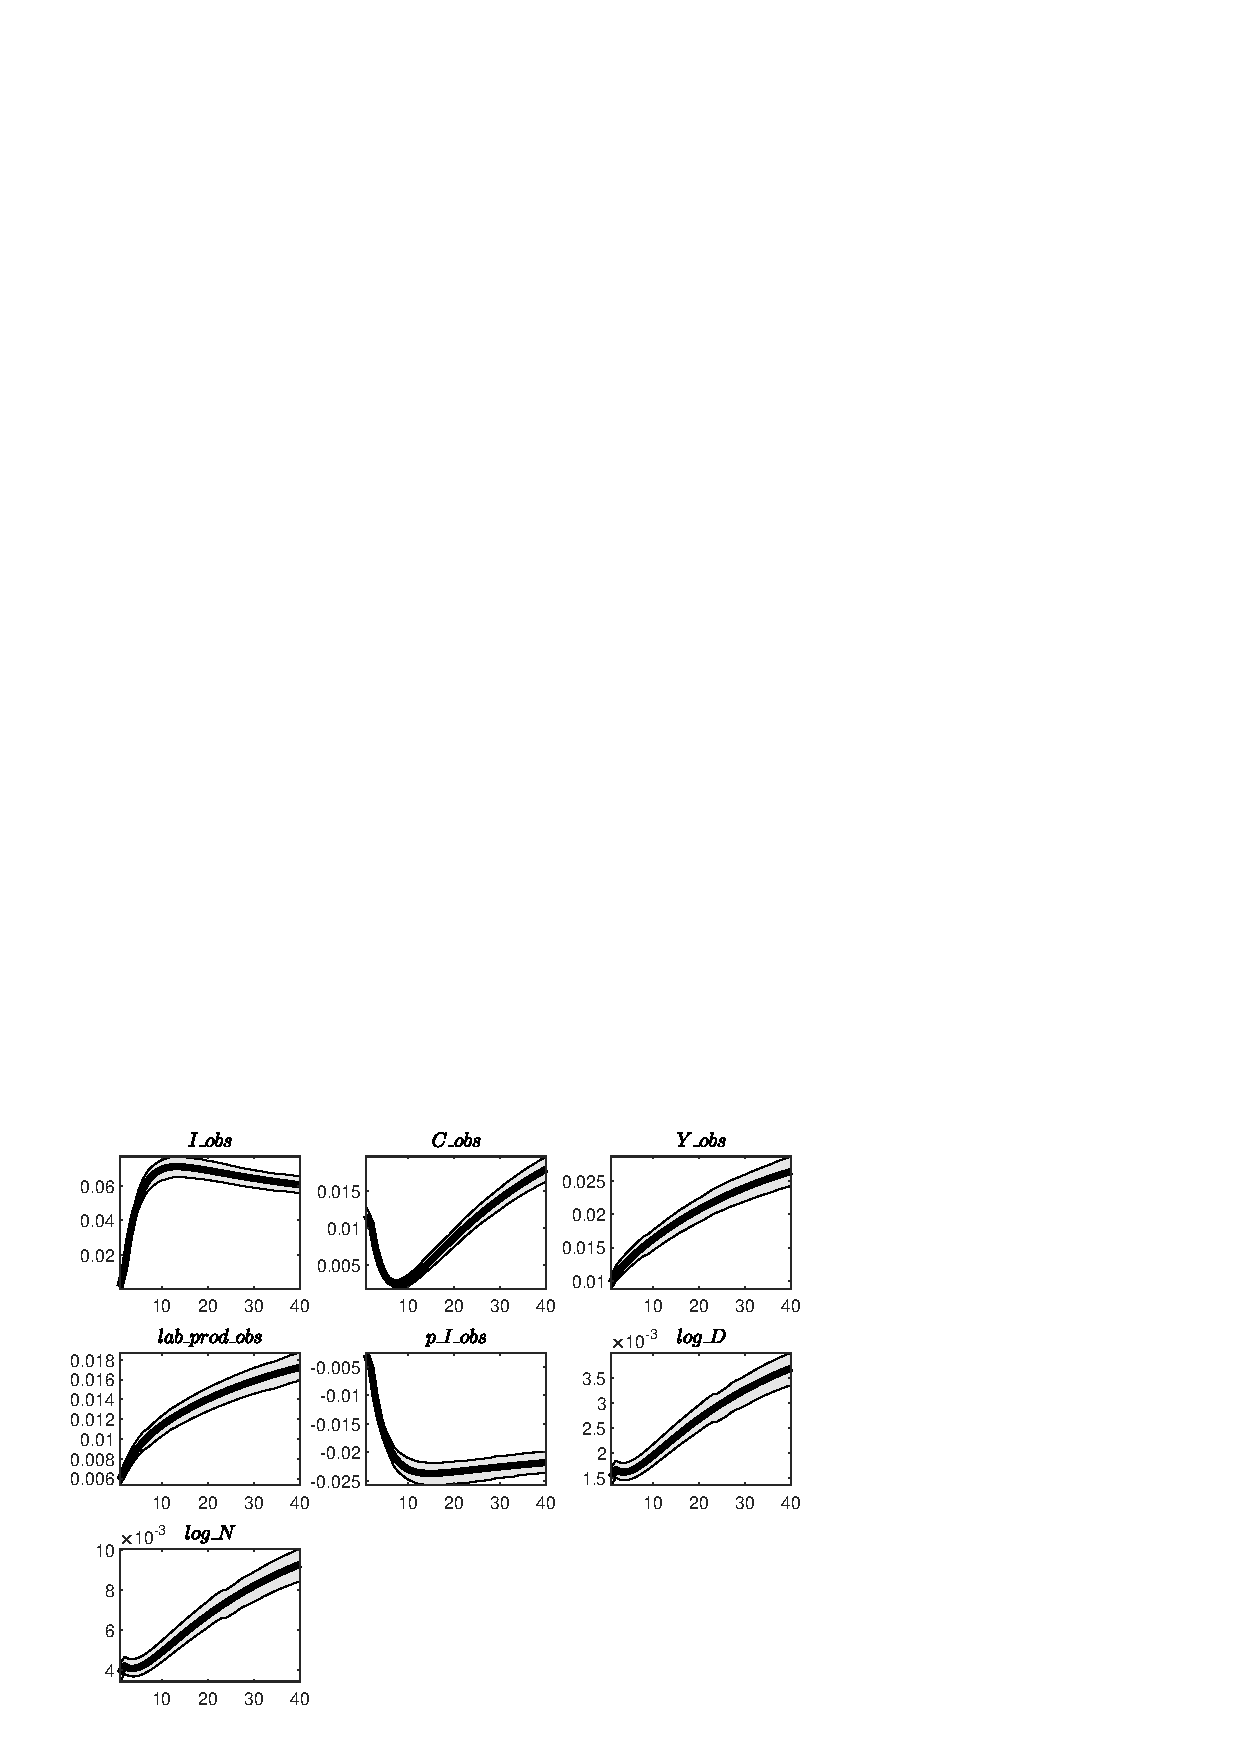
\includegraphics[width=0.80\textwidth]{BRS/Output/BRS_Bayesian_IRF_e_Z_1}
\caption{Bayesian IRF: Orthogonalized shock to ${e_Z}$.}
\label{Fig:BayesianIRF:e_Z:1}
\end{figure}
 
\begin{figure}[H]
\centering 
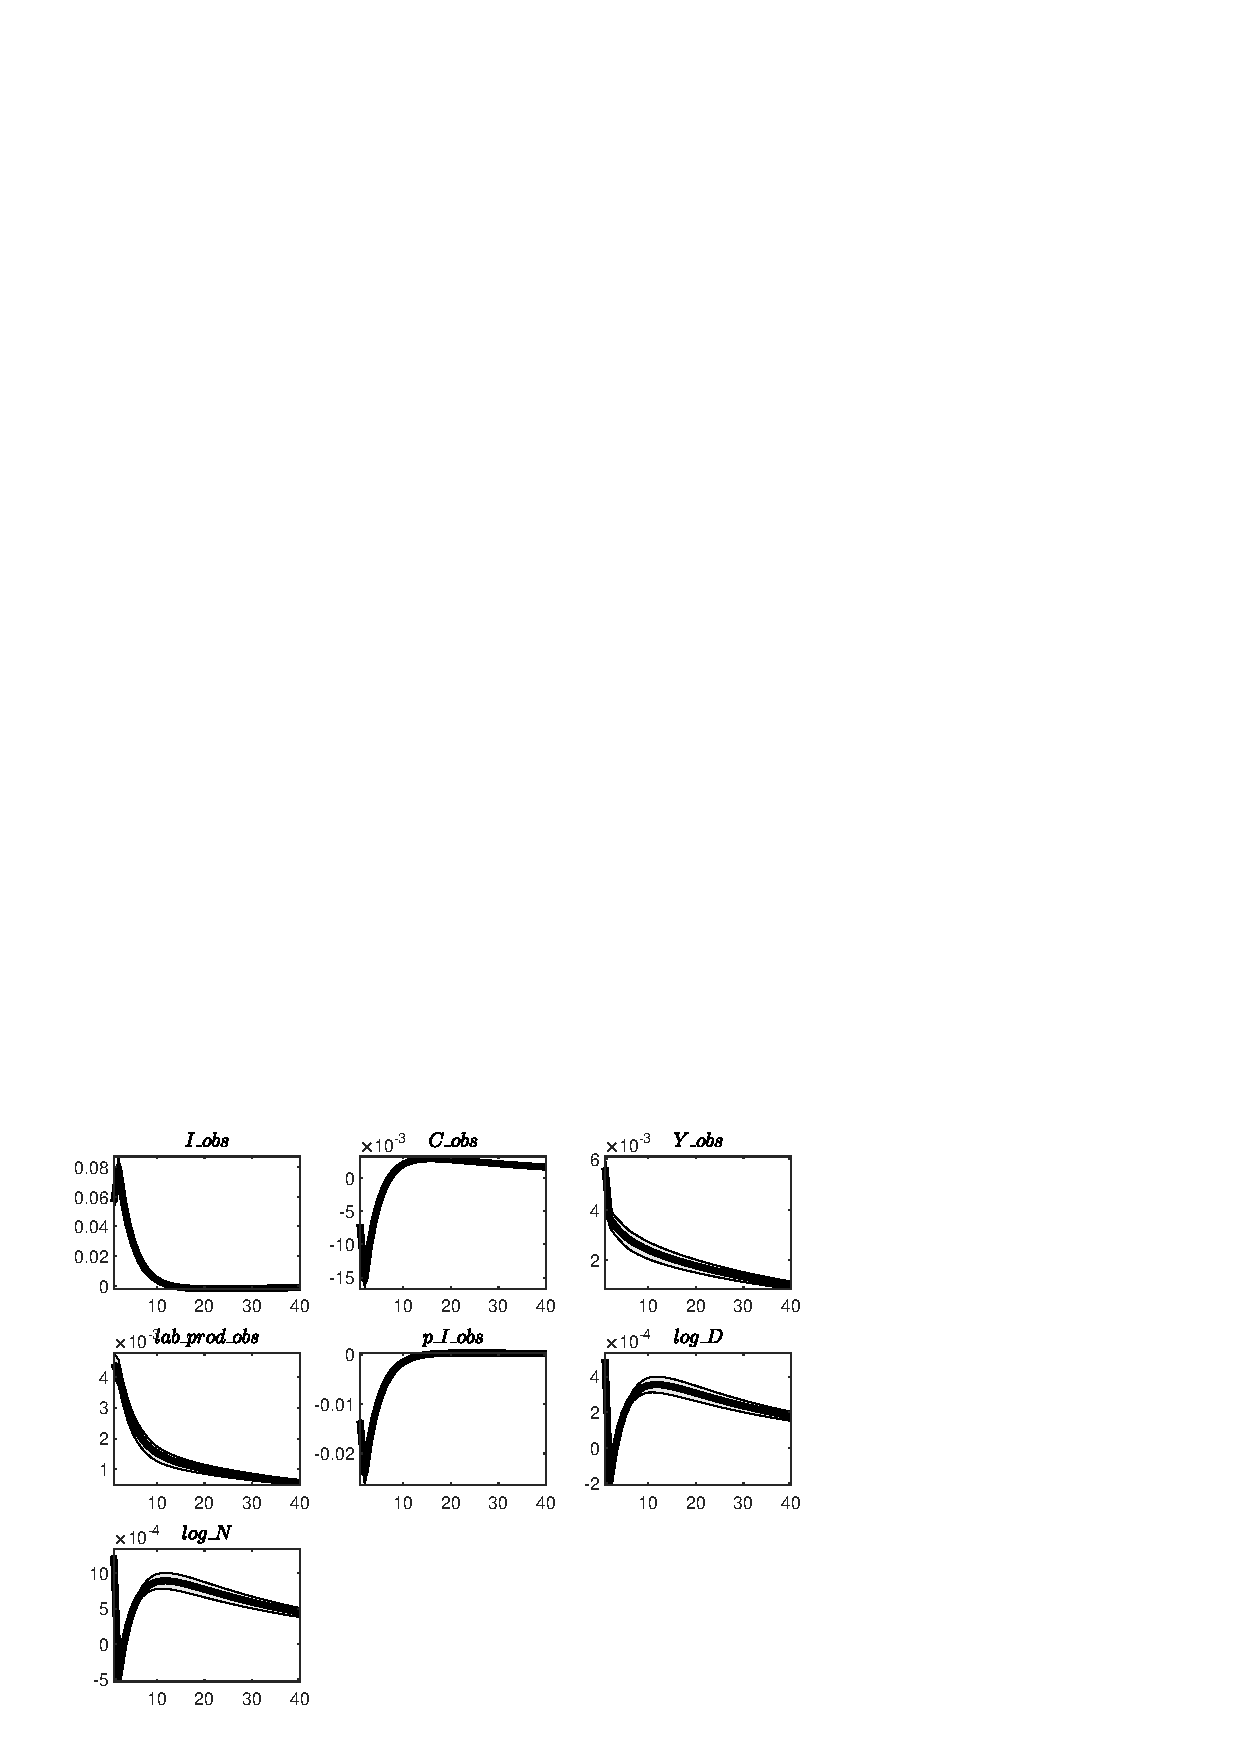
\includegraphics[width=0.80\textwidth]{BRS/Output/BRS_Bayesian_IRF_e_ZI_1}
\caption{Bayesian IRF: Orthogonalized shock to ${e_ZI}$.}
\label{Fig:BayesianIRF:e_ZI:1}
\end{figure}
 
\begin{figure}[H]
\centering 
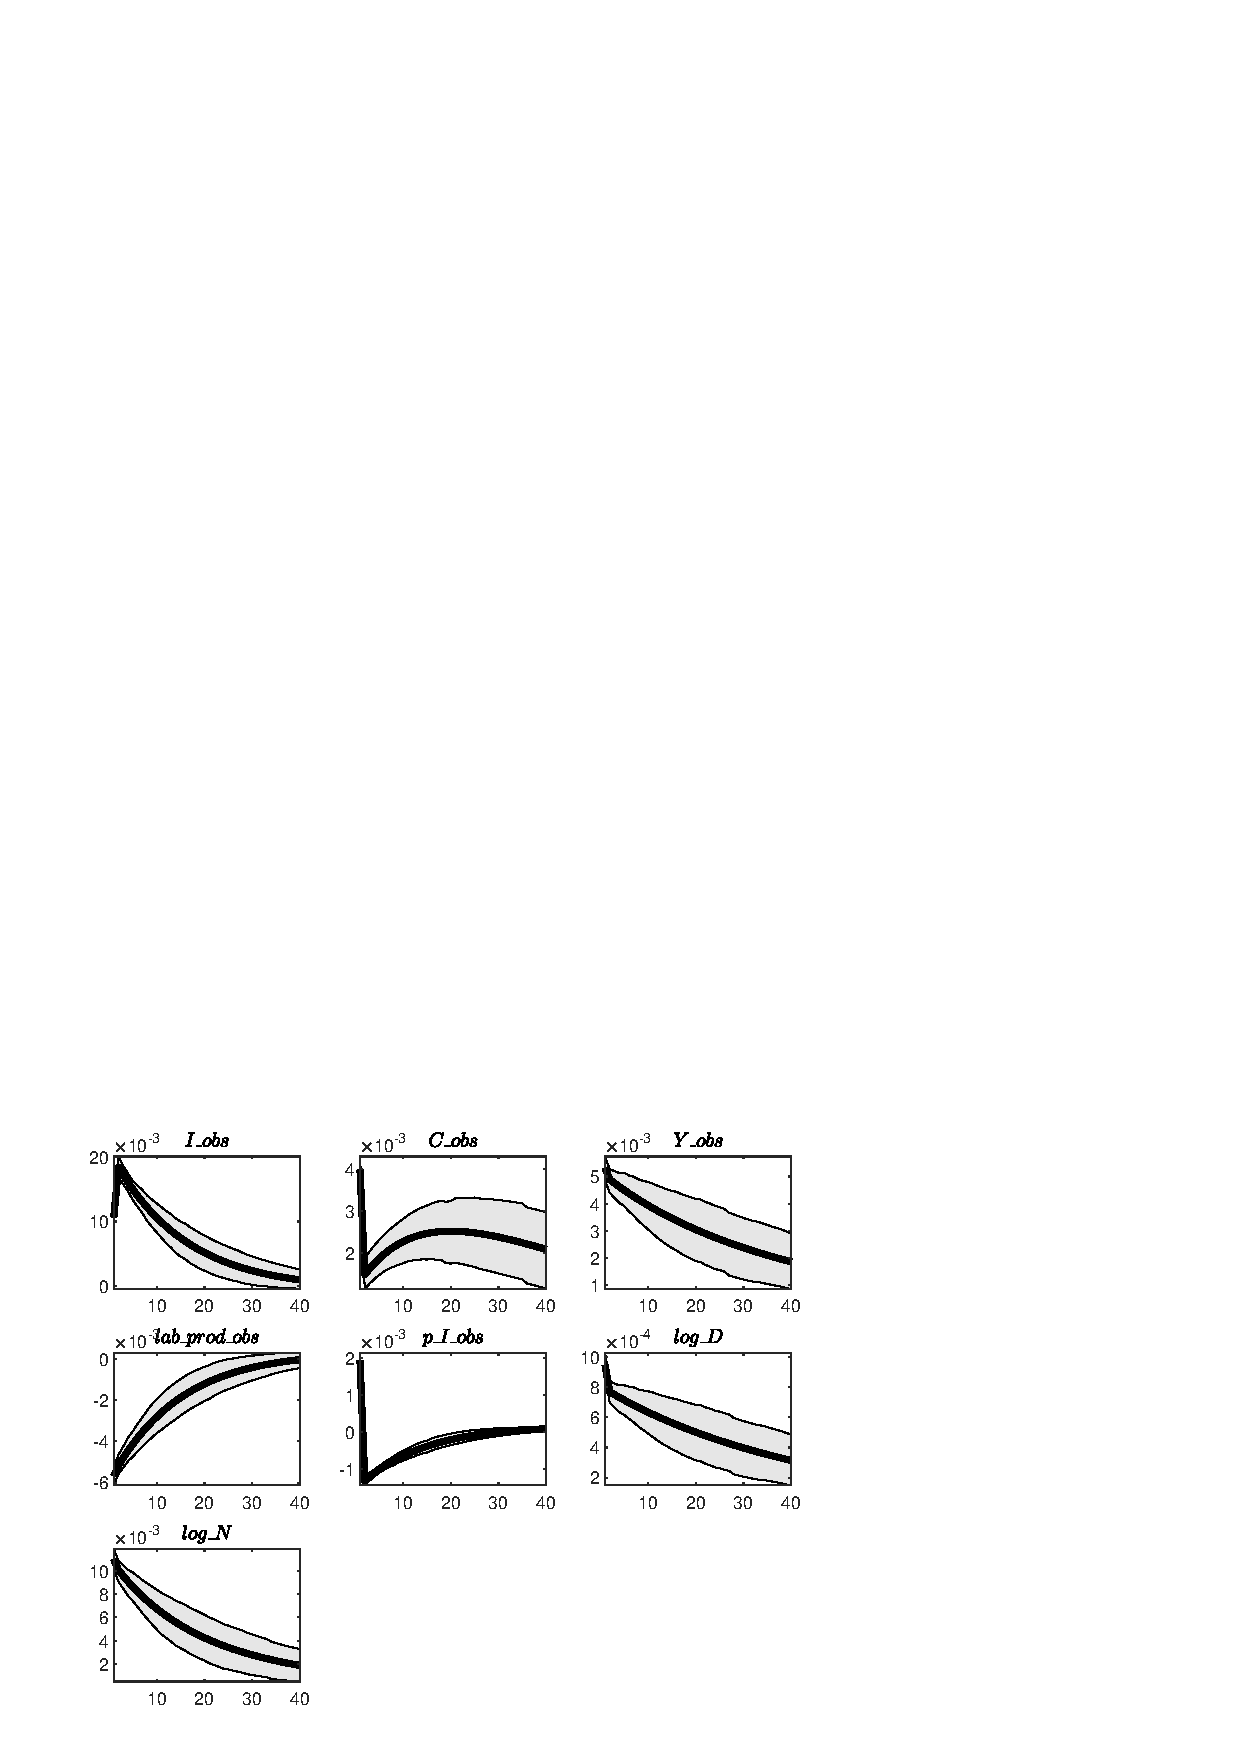
\includegraphics[width=0.80\textwidth]{BRS/Output/BRS_Bayesian_IRF_e_N_1}
\caption{Bayesian IRF: Orthogonalized shock to ${e_N}$.}
\label{Fig:BayesianIRF:e_N:1}
\end{figure}
 
\begin{figure}[H]
\centering 
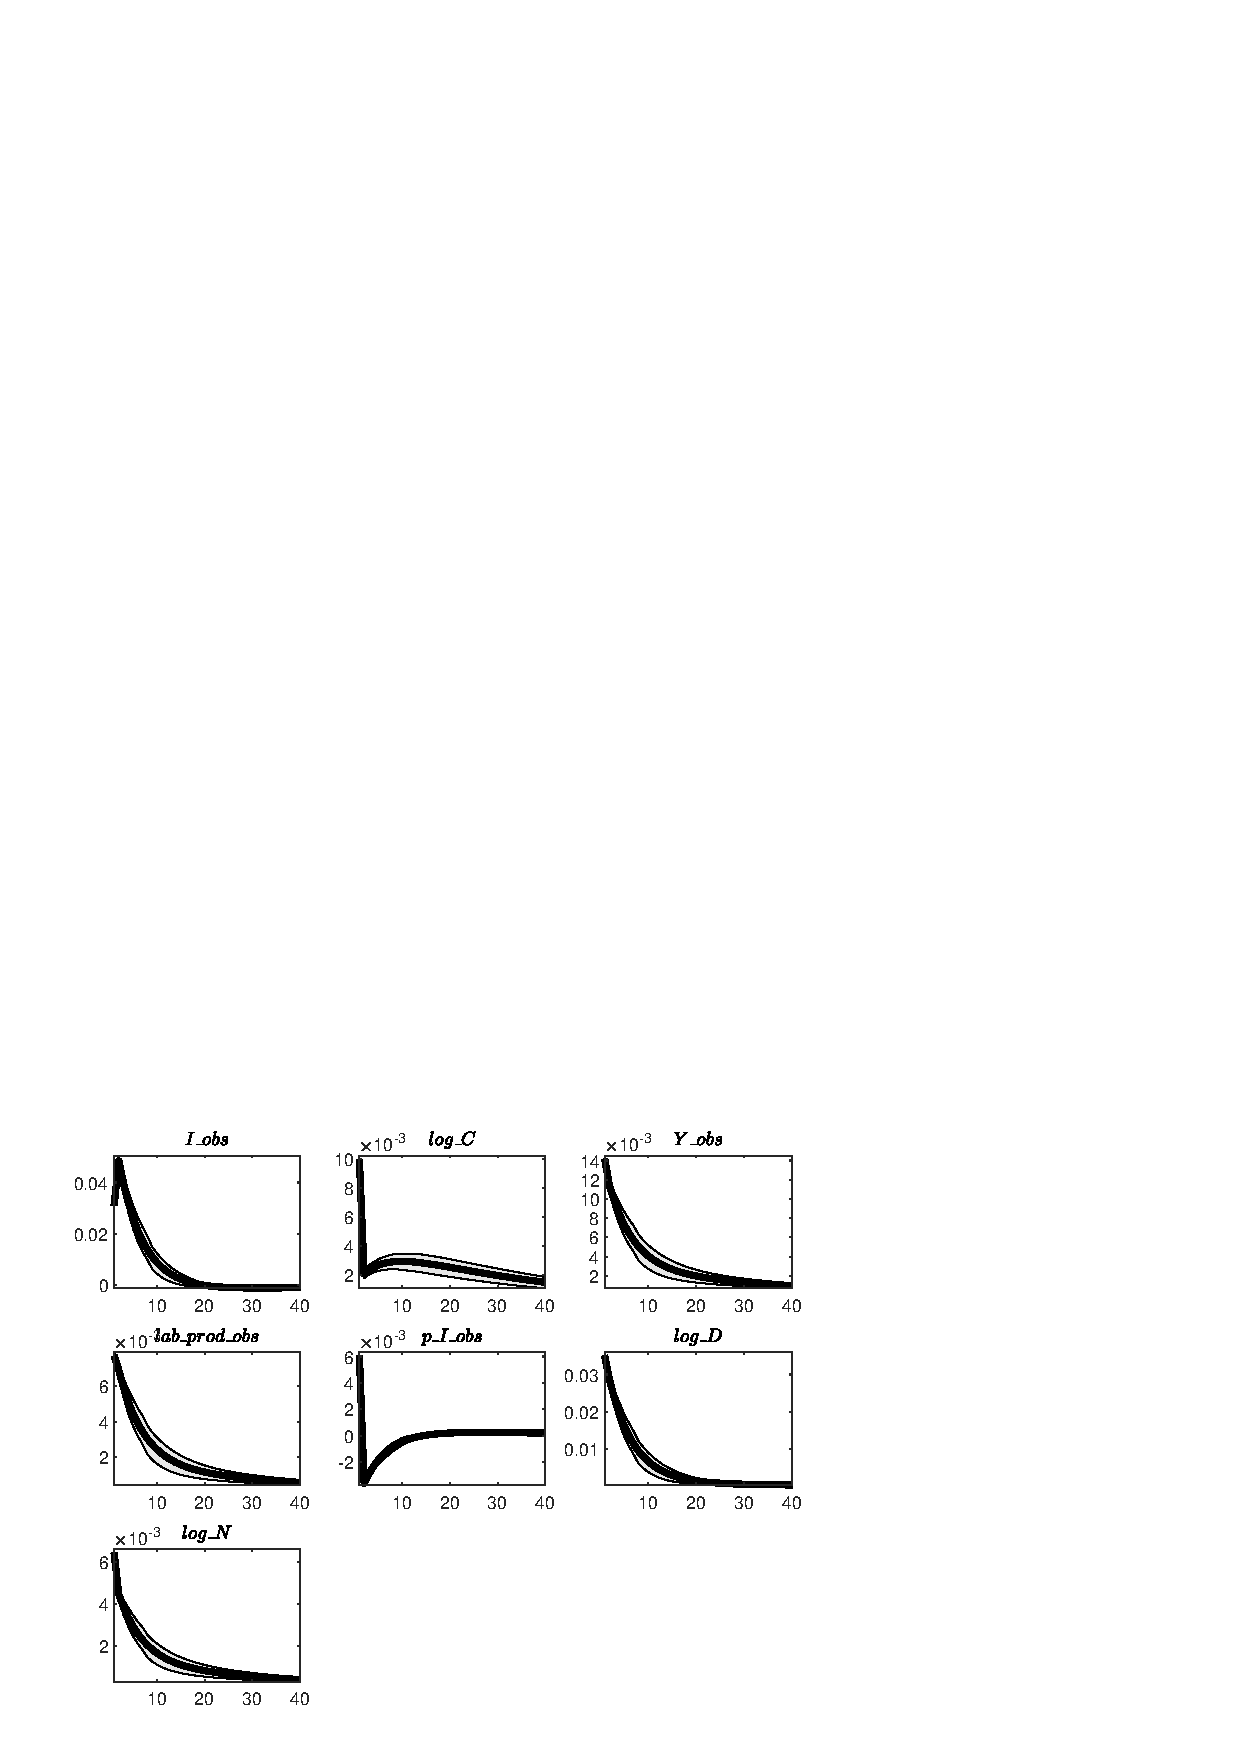
\includegraphics[width=0.80\textwidth]{BRS/Output/BRS_Bayesian_IRF_e_D_1}
\caption{Bayesian IRF: Orthogonalized shock to ${e_D}$.}
\label{Fig:BayesianIRF:e_D:1}
\end{figure}
 
% End of TeX file.
 
% TeX eps-loader file generated by McmcDiagnostics.m (Dynare).
% 19-Jan-2024 16:01:59
 
\begin{figure}[H]
\centering 
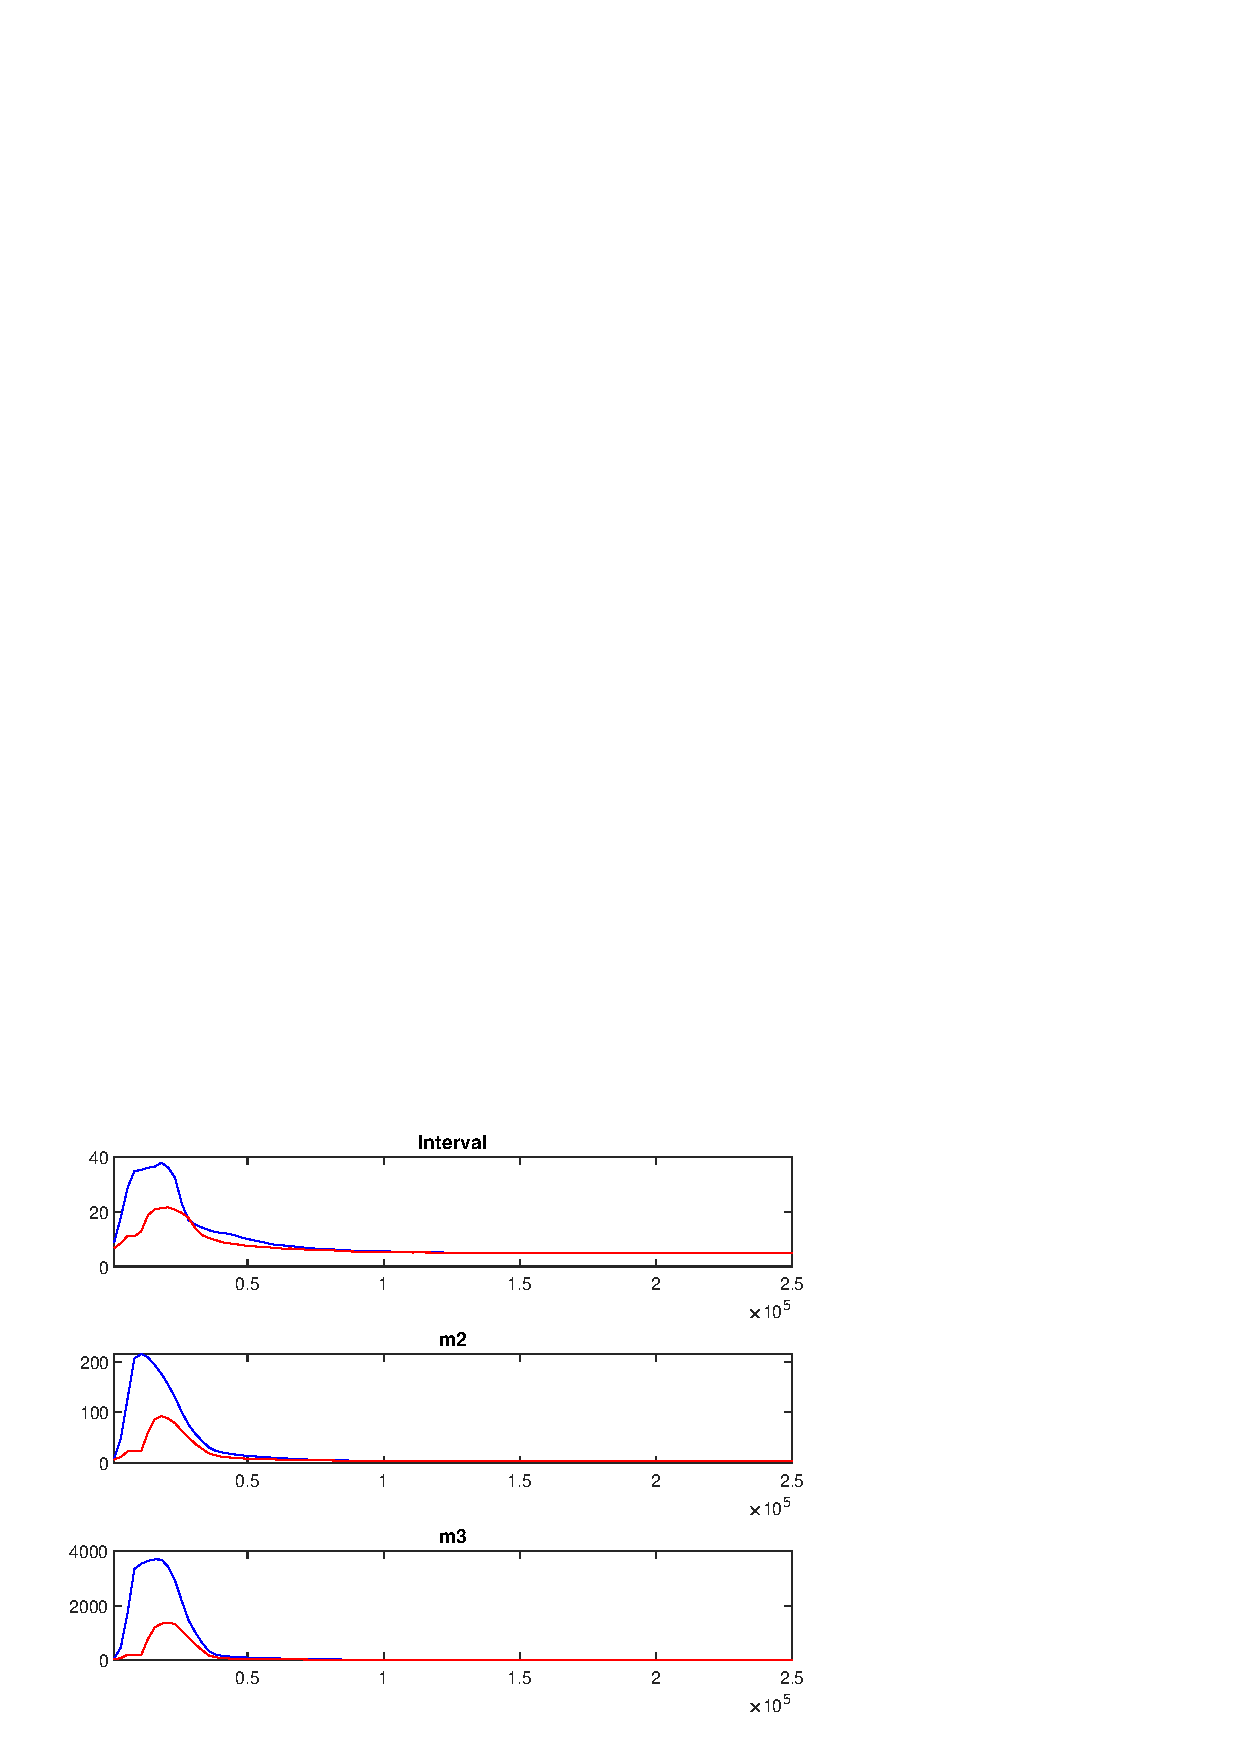
\includegraphics[width=0.8\textwidth]{BRS/Output/BRS_mdiag}
\caption{Multivariate convergence diagnostics for the Metropolis-Hastings.
The first, second and third rows are respectively the criteria based on
the eighty percent interval, the second and third moments. The different 
parameters are aggregated using the posterior kernel.}\label{Fig:MultivariateDiagnostics}
\end{figure}

% End Of TeX file. 
% TeX-table generated by Dynare.
% RESULTS FROM METROPOLIS HASTINGS (parameters)
% 21-Jan-2024 18:58:10 
 
\begin{center}
\begin{longtable}{llcccccc} 
\caption{Results from Metropolis-Hastings (parameters)}
 \label{Table:MHPosterior:1}\\
\toprule 
  & \multicolumn{3}{c}{Prior}  &  \multicolumn{4}{c}{Posterior} \\
  \cmidrule(r{.75em}){2-4} \cmidrule(r{.75em}){5-8}
  & Dist. & Mean  & Stdev. & Mean & Stdev. & HPD inf & HPD sup\\
\midrule \endfirsthead 
\caption{(continued)}\\\toprule 
  & \multicolumn{3}{c}{Prior}  &  \multicolumn{4}{c}{Posterior} \\
  \cmidrule(r{.75em}){2-4} \cmidrule(r{.75em}){5-8}
  & Dist. & Mean  & Stdev. & Mean & Stdev. & HPD inf & HPD sup\\
\midrule \endhead 
\bottomrule \multicolumn{8}{r}{(Continued on next page)} \endfoot 
\bottomrule \endlastfoot 
${\rho_Z}$ & beta &   0.600 & 0.2000 &   0.999& 0.0005 &  0.9985 &  0.9999 \\ 
${\rho_ZI}$ & beta &   0.600 & 0.2000 &   0.733& 0.0124 &  0.7125 &  0.7541 \\ 
${\rho_N}$ & beta &   0.600 & 0.2000 &   0.944& 0.0160 &  0.9184 &  0.9700 \\ 
${\rho_D}$ & beta &   0.600 & 0.2000 &   0.825& 0.0243 &  0.7861 &  0.8657 \\ 
\end{longtable}
 \end{center}
% End of TeX file.
 
% TeX-table generated by Dynare.
% RESULTS FROM METROPOLIS HASTINGS (standard deviation of structural shocks)
% 21-Jan-2024 18:58:14 
 
\begin{center}
\begin{longtable}{llcccccc} 
\caption{Results from Metropolis-Hastings (standard deviation of structural shocks)}
 \label{Table:MHPosterior:2}\\
\toprule 
  & \multicolumn{3}{c}{Prior}  &  \multicolumn{4}{c}{Posterior} \\
  \cmidrule(r{.75em}){2-4} \cmidrule(r{.75em}){5-8}
  & Dist. & Mean  & Stdev. & Mean & Stdev. & HPD inf & HPD sup\\
\midrule \endfirsthead 
\caption{(continued)}\\\toprule 
  & \multicolumn{3}{c}{Prior}  &  \multicolumn{4}{c}{Posterior} \\
  \cmidrule(r{.75em}){2-4} \cmidrule(r{.75em}){5-8}
  & Dist. & Mean  & Stdev. & Mean & Stdev. & HPD inf & HPD sup\\
\midrule \endhead 
\bottomrule \multicolumn{8}{r}{(Continued on next page)} \endfoot 
\bottomrule \endlastfoot 
${e_ZI}$ & invg &   0.010 & 0.1000 &   0.025& 0.0013 &  0.0224 &  0.0266 \\ 
${e_Z}$ & invg &   0.010 & 0.1000 &   0.008& 0.0005 &  0.0067 &  0.0083 \\ 
${e_N}$ & invg &   0.010 & 0.1000 &   0.021& 0.0011 &  0.0187 &  0.0221 \\ 
${e_D}$ & invg &   0.010 & 0.1000 &   0.195& 0.0040 &  0.1899 &  0.2000 \\ 
\end{longtable}
 \end{center}
% End of TeX file.
 
% TeX-table generated by dynare_estimation (Dynare).
% RESULTS FROM POSTERIOR MAXIMIZATION (parameters)
% 21-Jan-2024 18:57:14 
 
\begin{center}
\begin{longtable}{llcccc} 
\caption{Results from posterior maximization (parameters)}\\
 \label{Table:Posterior:1}\\
\toprule 
  & \multicolumn{3}{c}{Prior}  &  \multicolumn{2}{c}{Posterior} \\
  \cmidrule(r{.75em}){2-4} \cmidrule(r{.75em}){5-6}
  & Dist. & Mean  & Stdev & Mode & Stdev \\ 
\midrule \endfirsthead 
\caption{(continued)}\\
 \bottomrule 
  & \multicolumn{3}{c}{Prior}  &  \multicolumn{2}{c}{Posterior} \\
  \cmidrule(r{.75em}){2-4} \cmidrule(r{.75em}){5-6}
  & Dist. & Mean  & Stdev & Mode & Stdev \\ 
\midrule \endhead 
\bottomrule \multicolumn{6}{r}{(Continued on next page)}\endfoot 
\bottomrule\endlastfoot 
${\rho_Z}$ & beta &   0.600 & 0.2000 &   0.8997 &  0.0313 \\ 
${\rho_ZI}$ & beta &   0.600 & 0.2000 &   0.9729 &  0.0138 \\ 
${\rho_N}$ & beta &   0.600 & 0.2000 &   0.9458 &  0.0174 \\ 
${\rho_D}$ & beta &   0.600 & 0.2000 &   0.7819 &  0.0399 \\ 
\end{longtable}
 \end{center}
% End of TeX file.
 
% TeX-table generated by dynare_estimation (Dynare).
% RESULTS FROM POSTERIOR MAXIMIZATION (standard deviation of structural shocks)
% 19-Jan-2024 15:47:58 
 
\begin{center}
\begin{longtable}{llcccc} 
\caption{Results from posterior maximization (standard deviation of structural shocks)}\\
 \label{Table:Posterior:2}\\
\toprule 
  & \multicolumn{3}{c}{Prior}  &  \multicolumn{2}{c}{Posterior} \\
  \cmidrule(r{.75em}){2-4} \cmidrule(r{.75em}){5-6}
  & Dist. & Mean  & Stdev & Mode & Stdev \\ 
\midrule \endfirsthead 
\caption{(continued)}\\
 \bottomrule 
  & \multicolumn{3}{c}{Prior}  &  \multicolumn{2}{c}{Posterior} \\
  \cmidrule(r{.75em}){2-4} \cmidrule(r{.75em}){5-6}
  & Dist. & Mean  & Stdev & Mode & Stdev \\ 
\midrule \endhead 
\bottomrule \multicolumn{6}{r}{(Continued on next page)}\endfoot 
\bottomrule\endlastfoot 
${e_ZI}$ & invg &   0.010 & 0.1000 &   0.0306 &  0.0019 \\ 
${e_Z}$ & invg &   0.010 & 0.1000 &   0.0062 &  0.0006 \\ 
${e_N}$ & invg &   0.010 & 0.1000 &   0.0203 &  0.0010 \\ 
${e_D}$ & invg &   0.010 & 0.1000 &   0.1978 &  0.0102 \\ 
\end{longtable}
 \end{center}
% End of TeX file.
 
% TeX eps-loader file generated by PlotPosteriorDistributions.m (Dynare).
% 19-Jan-2024 16:02:07
 
\begin{figure}[H]
\centering
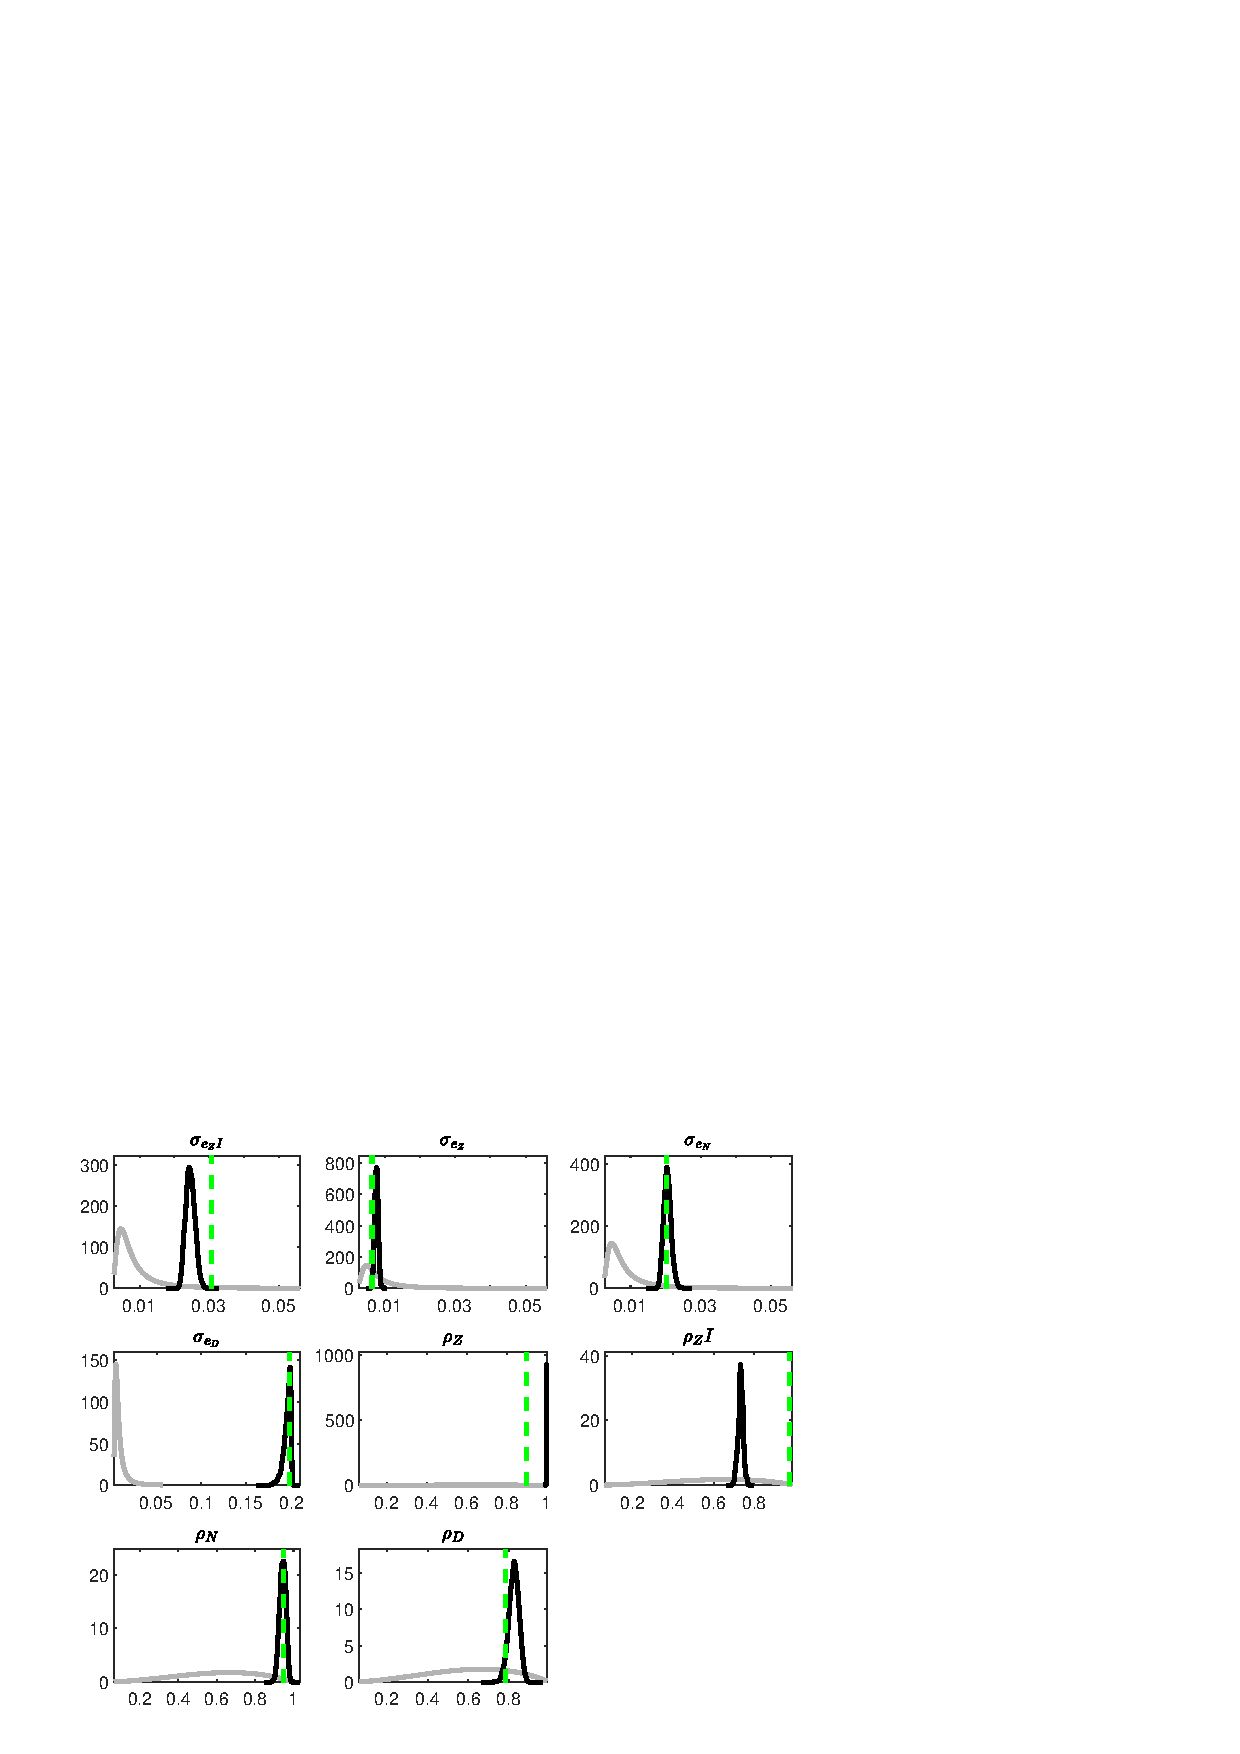
\includegraphics[width=0.80\textwidth]{BRS/Output/BRS_PriorsAndPosteriors1}
\caption{Priors and posteriors.}\label{Fig:PriorsAndPosteriors:1}
\end{figure}
 
% End of TeX file.
 
% TeX eps-loader file generated by McmcDiagnostics.m (Dynare).
% 23-Jan-2024 12:11:56
 
\begin{figure}[H]
\centering 
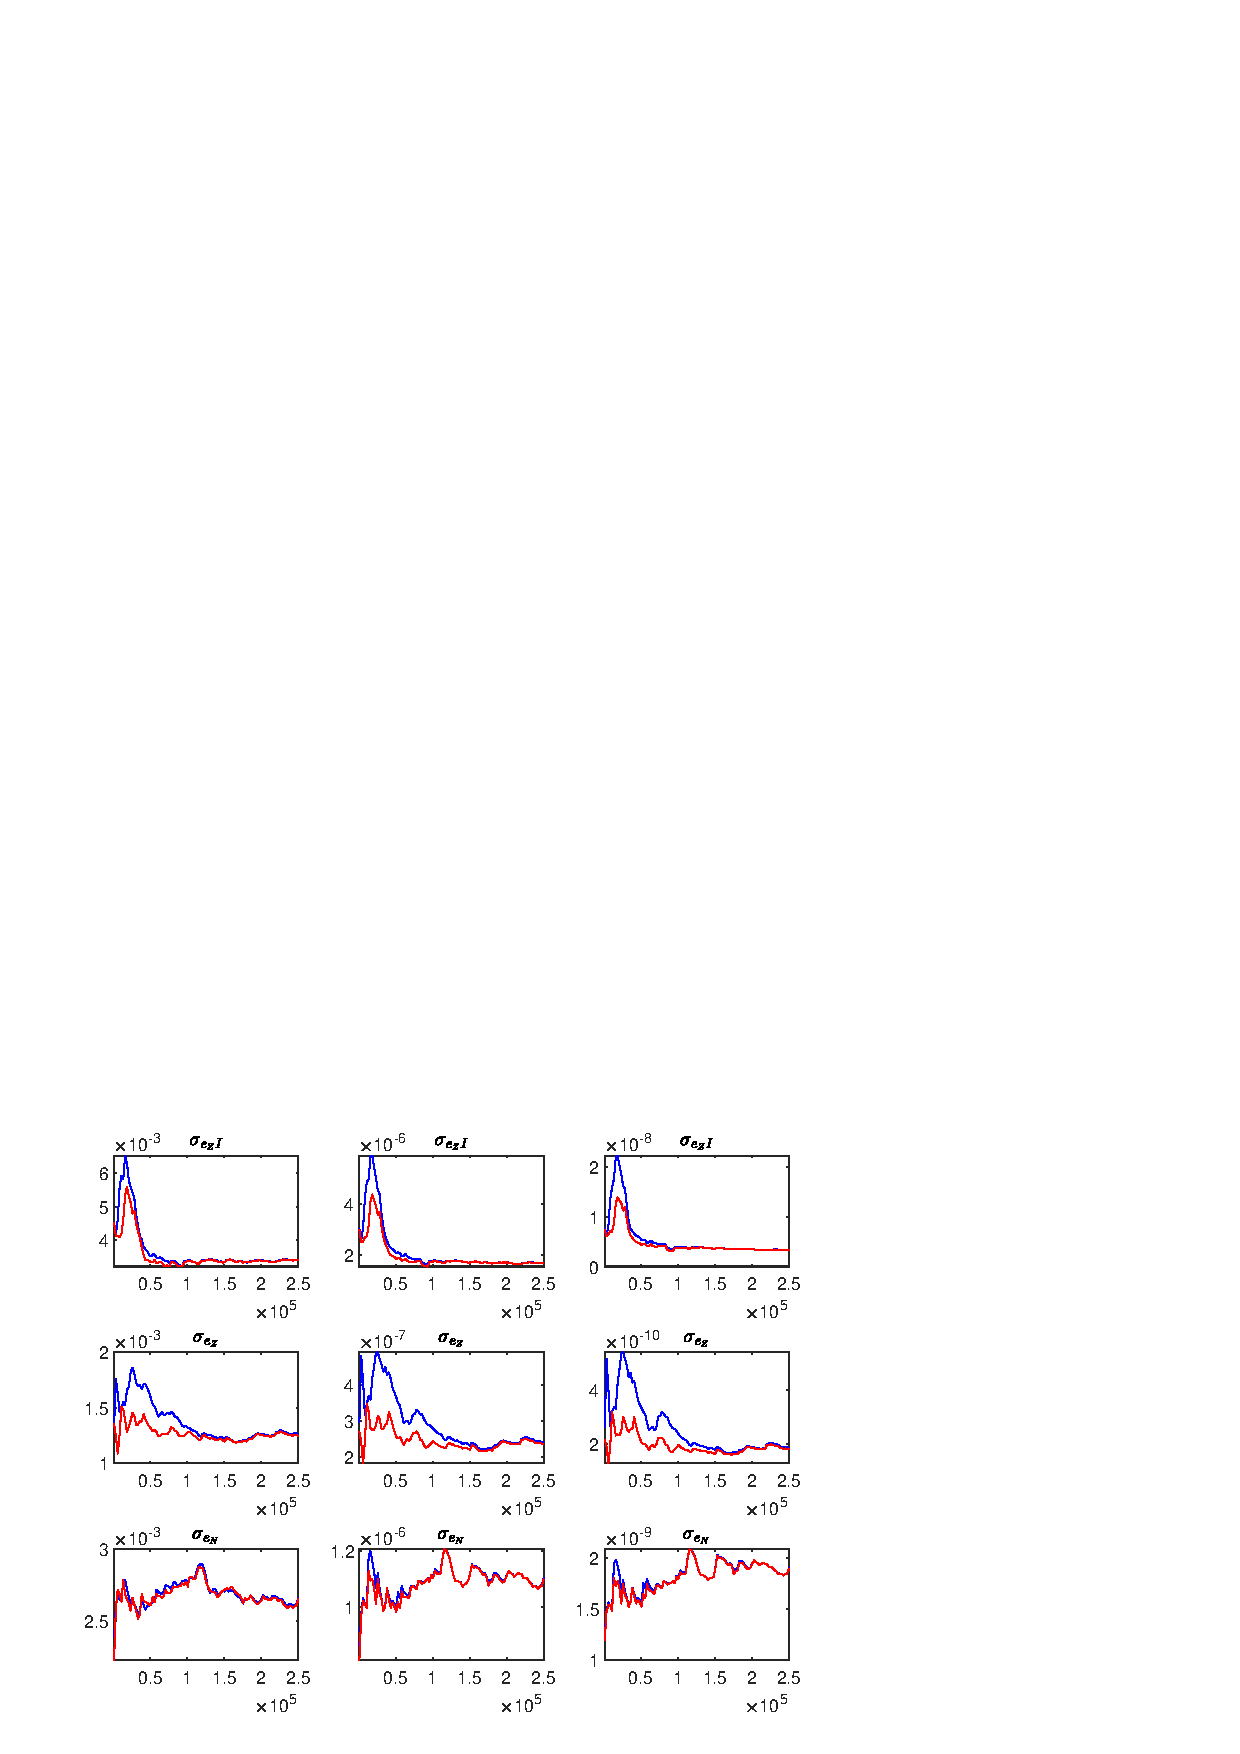
\includegraphics[width=0.80\textwidth]{BRS/Output/BRS_udiag1}
\caption{Univariate convergence diagnostics for the Metropolis-Hastings.
The first, second and third columns are respectively the criteria based on
the eighty percent interval, the second and third moments.}\label{Fig:UnivariateDiagnostics:1}
\end{figure}

\begin{figure}[H]
\centering 
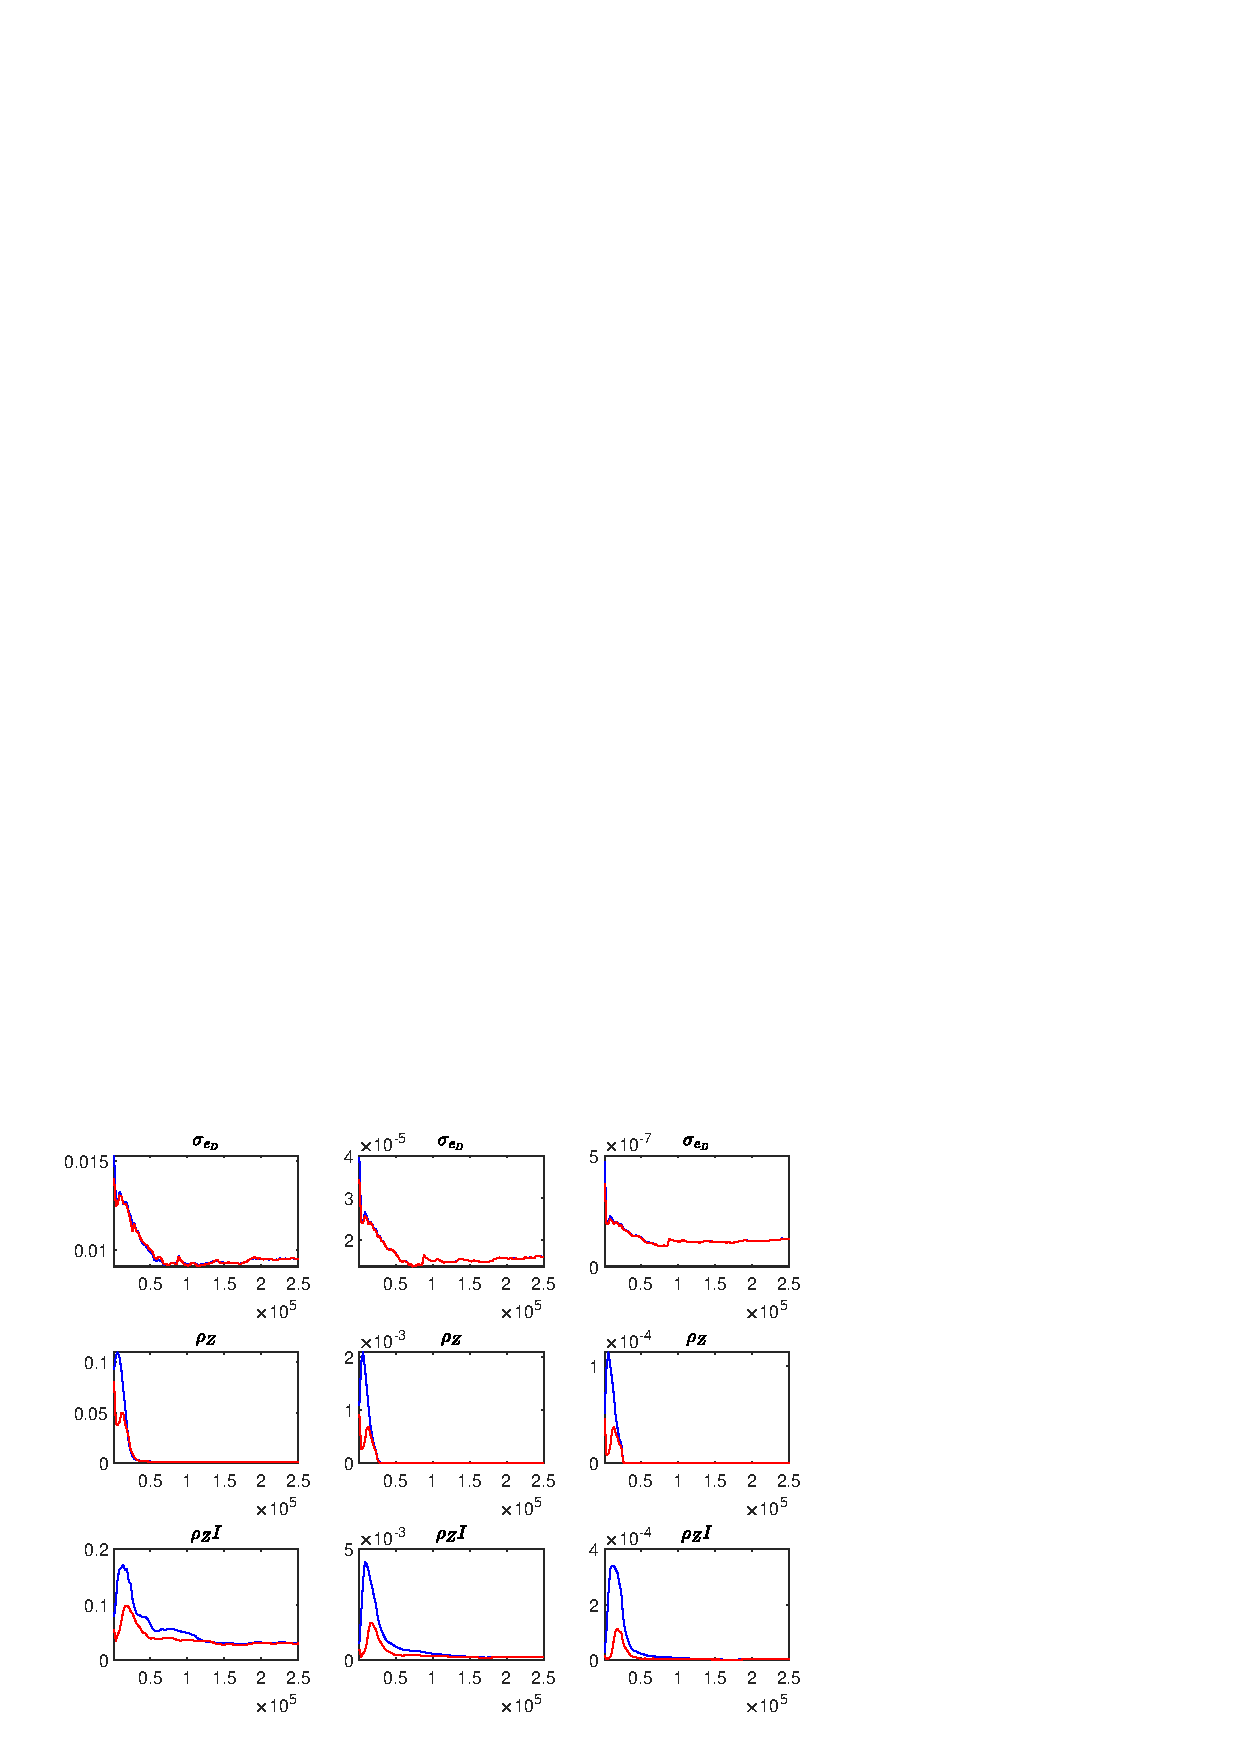
\includegraphics[width=0.80\textwidth]{BRS/Output/BRS_udiag2}
\caption{Univariate convergence diagnostics for the Metropolis-Hastings.
The first, second and third columns are respectively the criteria based on
the eighty percent interval, the second and third moments.}\label{Fig:UnivariateDiagnostics:2}
\end{figure}

\begin{figure}[H]
\centering 
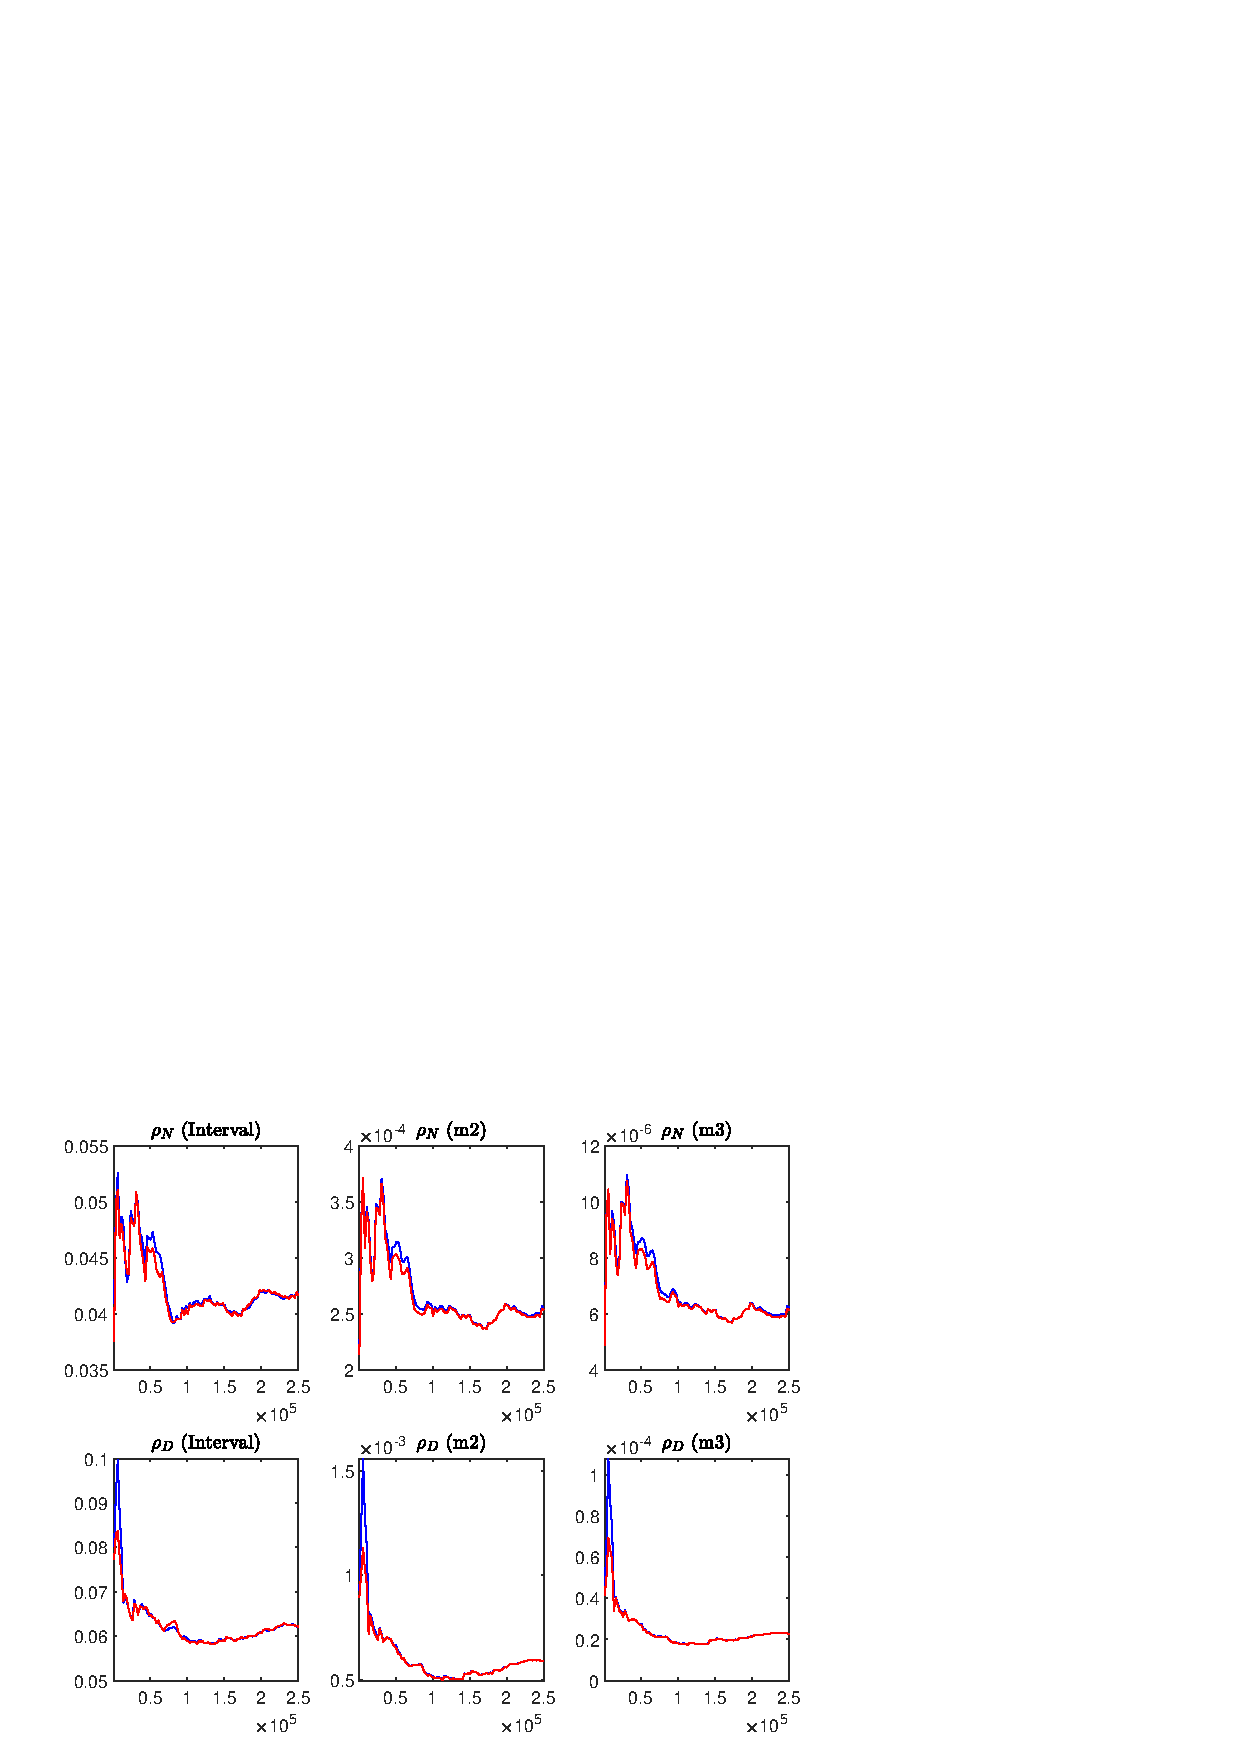
\includegraphics[width=0.80\textwidth]{BRS/Output/BRS_udiag3}
\caption{Univariate convergence diagnostics for the Metropolis-Hastings.
The first, second and third columns are respectively the criteria based on
the eighty percent interval, the second and third moments.}\label{Fig:UnivariateDiagnostics:3}
\end{figure}

 
% TeX eps-loader file generated by mode_check.m (Dynare).
% 23-Jan-2024 16:35:00
 
\begin{figure}[H]
\centering 
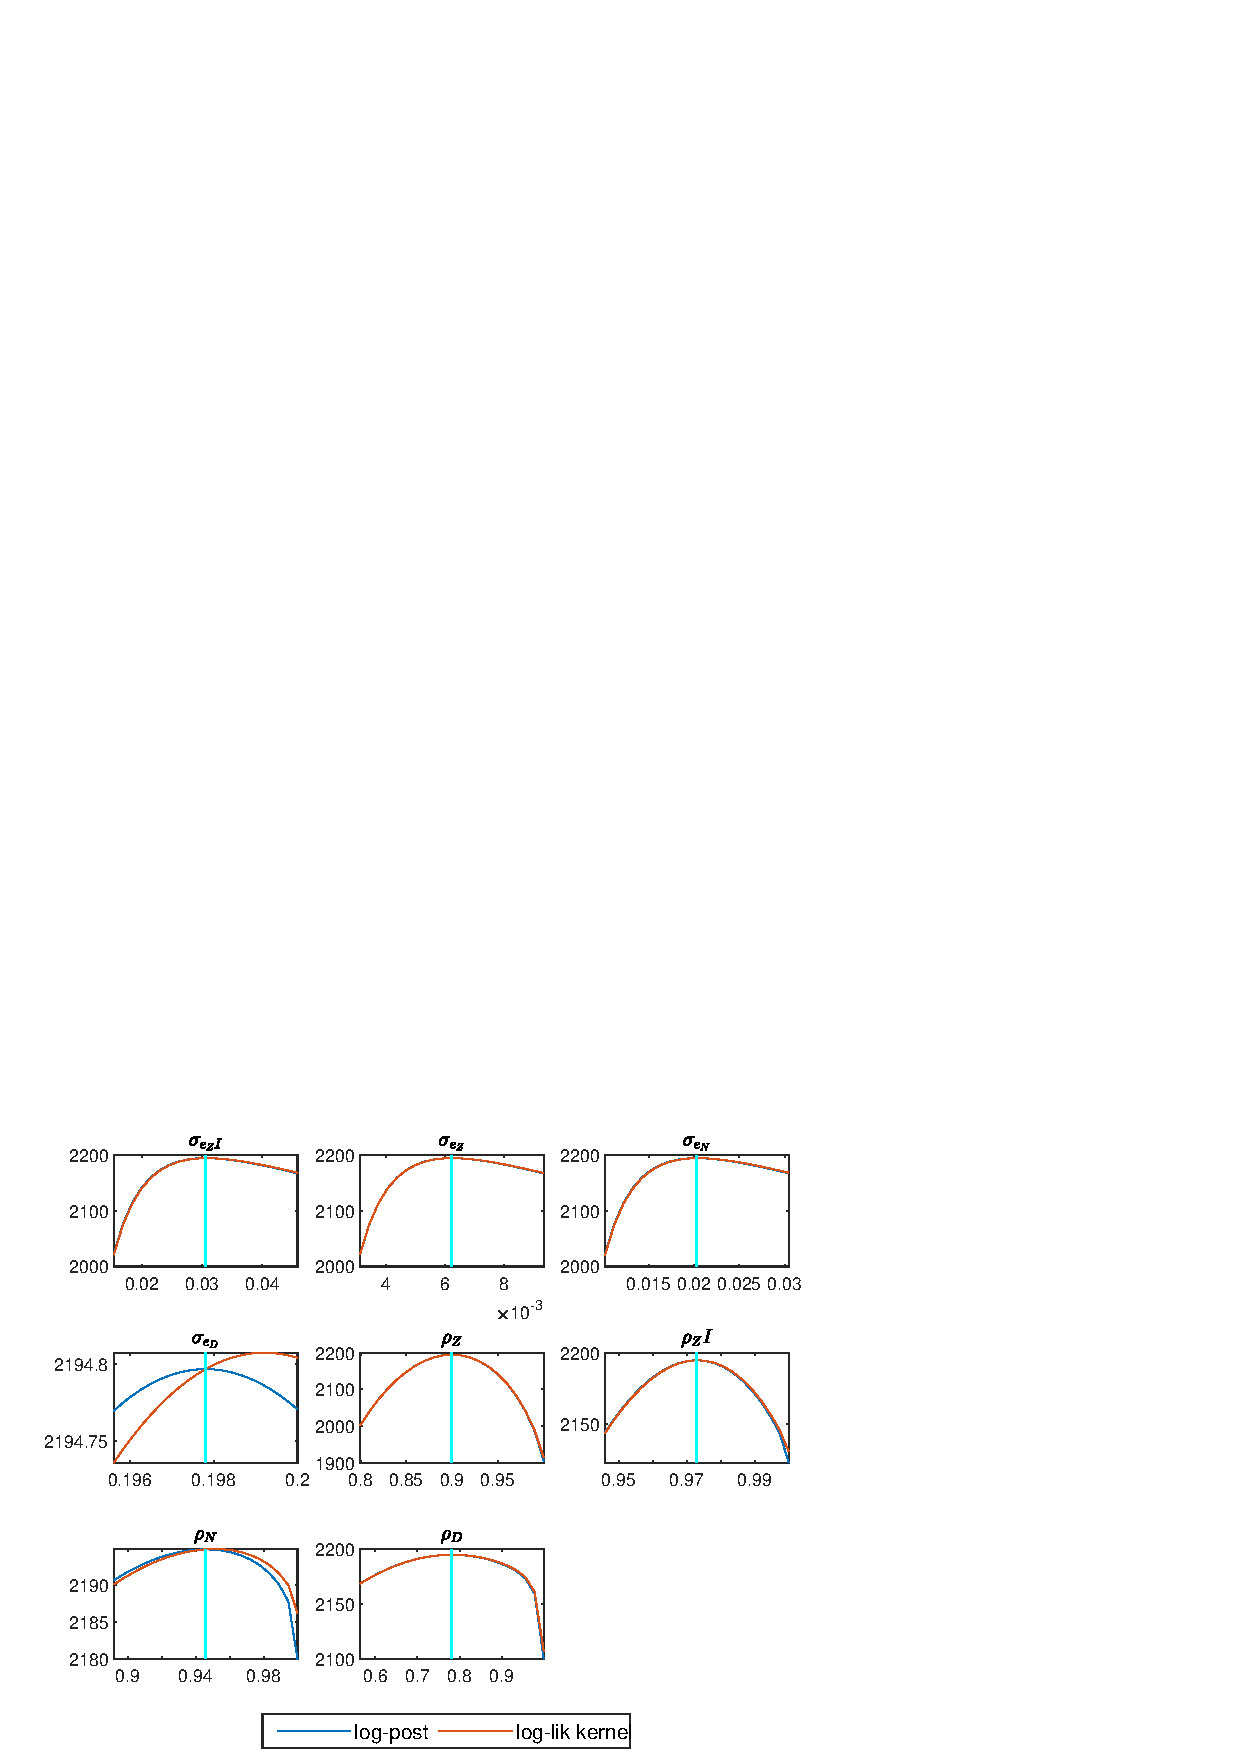
\includegraphics[width=0.80\textwidth]{BRS/graphs/BRS_CheckPlots1}
\caption{Check plots.}\label{Fig:CheckPlots:1}
\end{figure}
 
 
% TeX eps-loader file generated by dynare_estimation_1.m (Dynare).
% 21-Jan-2024 18:59:26
 
\begin{figure}[H]
\centering 
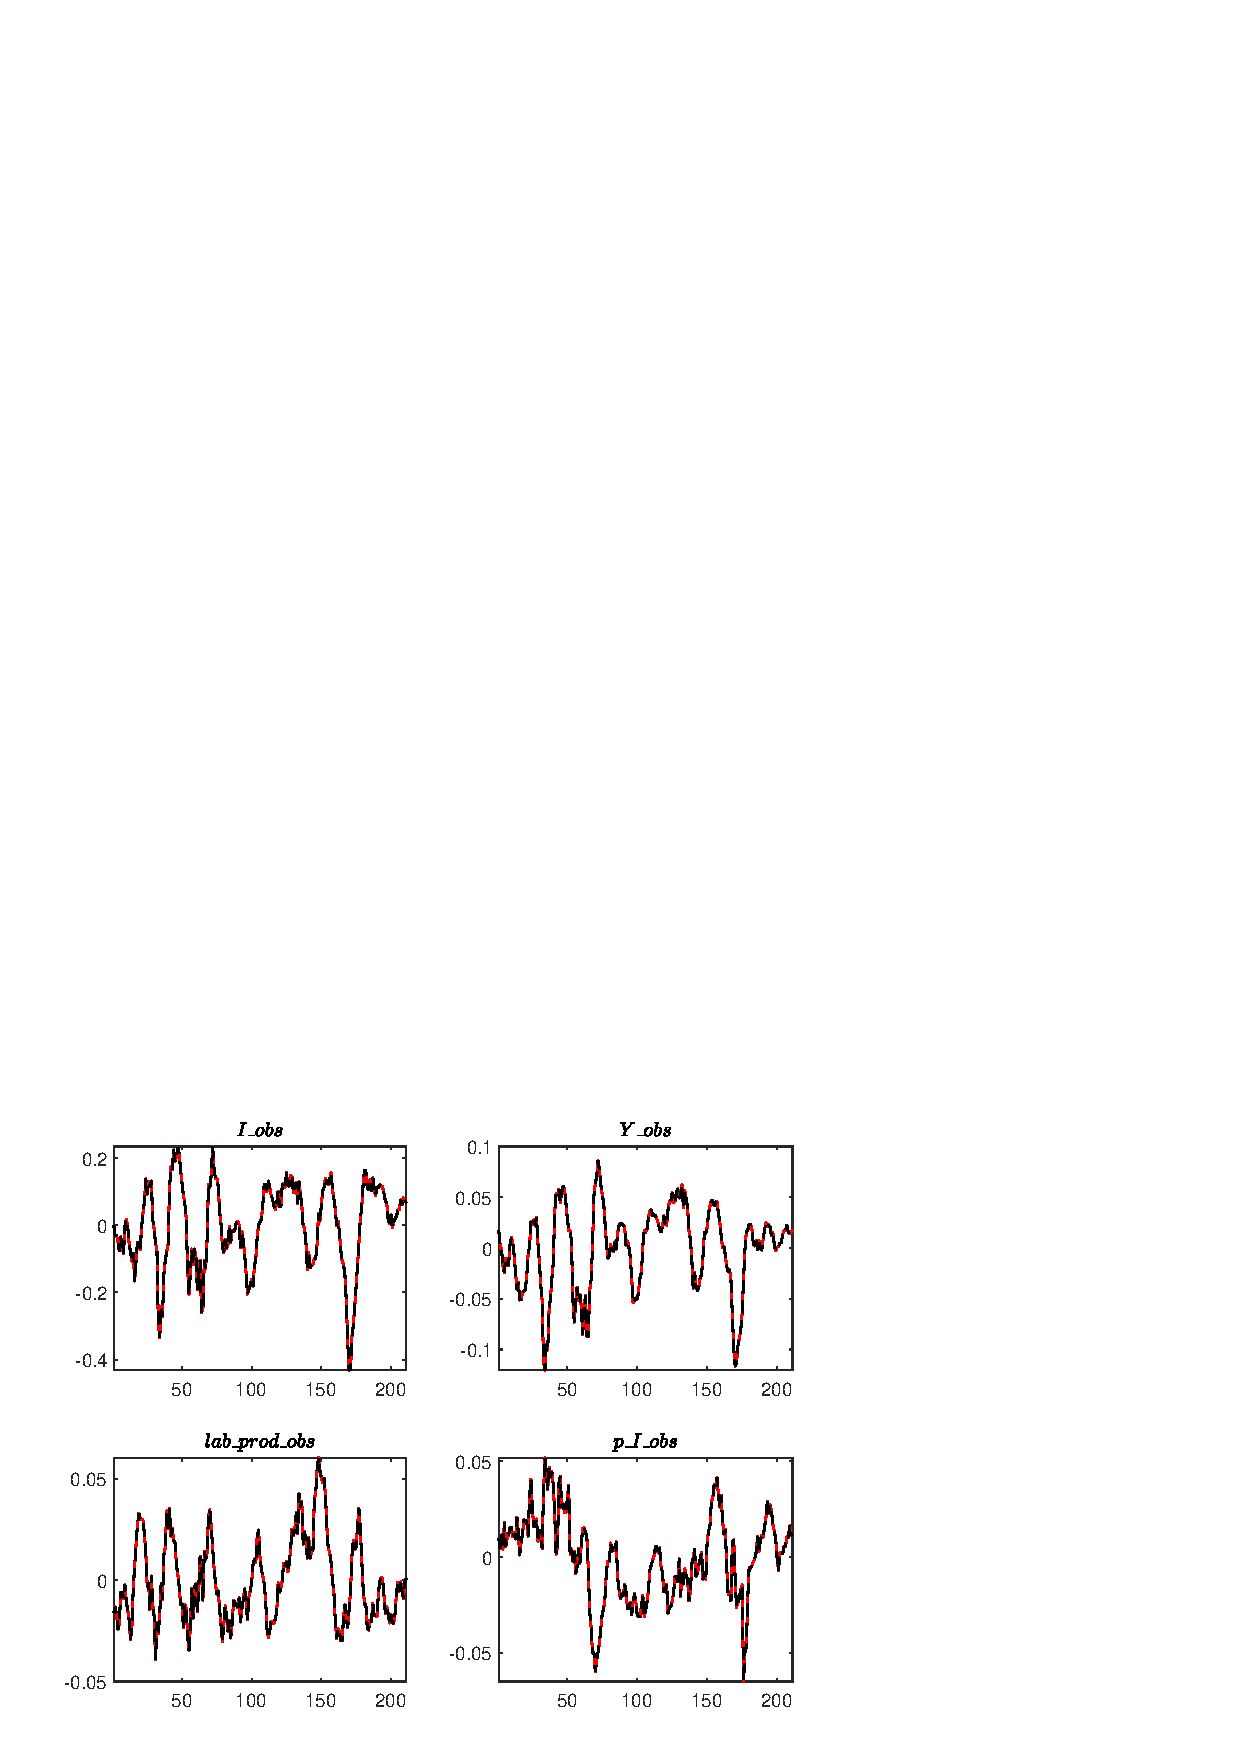
\includegraphics[width=0.80\textwidth]{BRS/graphs/BRS_HistoricalAndSmoothedVariables1}
\caption{Historical and smoothed variables.}\label{Fig:HistoricalAndSmoothedVariables:1}
\end{figure}


% End of TeX file.
 
% TeX eps-loader file generated by stoch_simul.m (Dynare).
% 19-Jan-2024 16:02:48
 
\begin{figure}[H]
\centering 
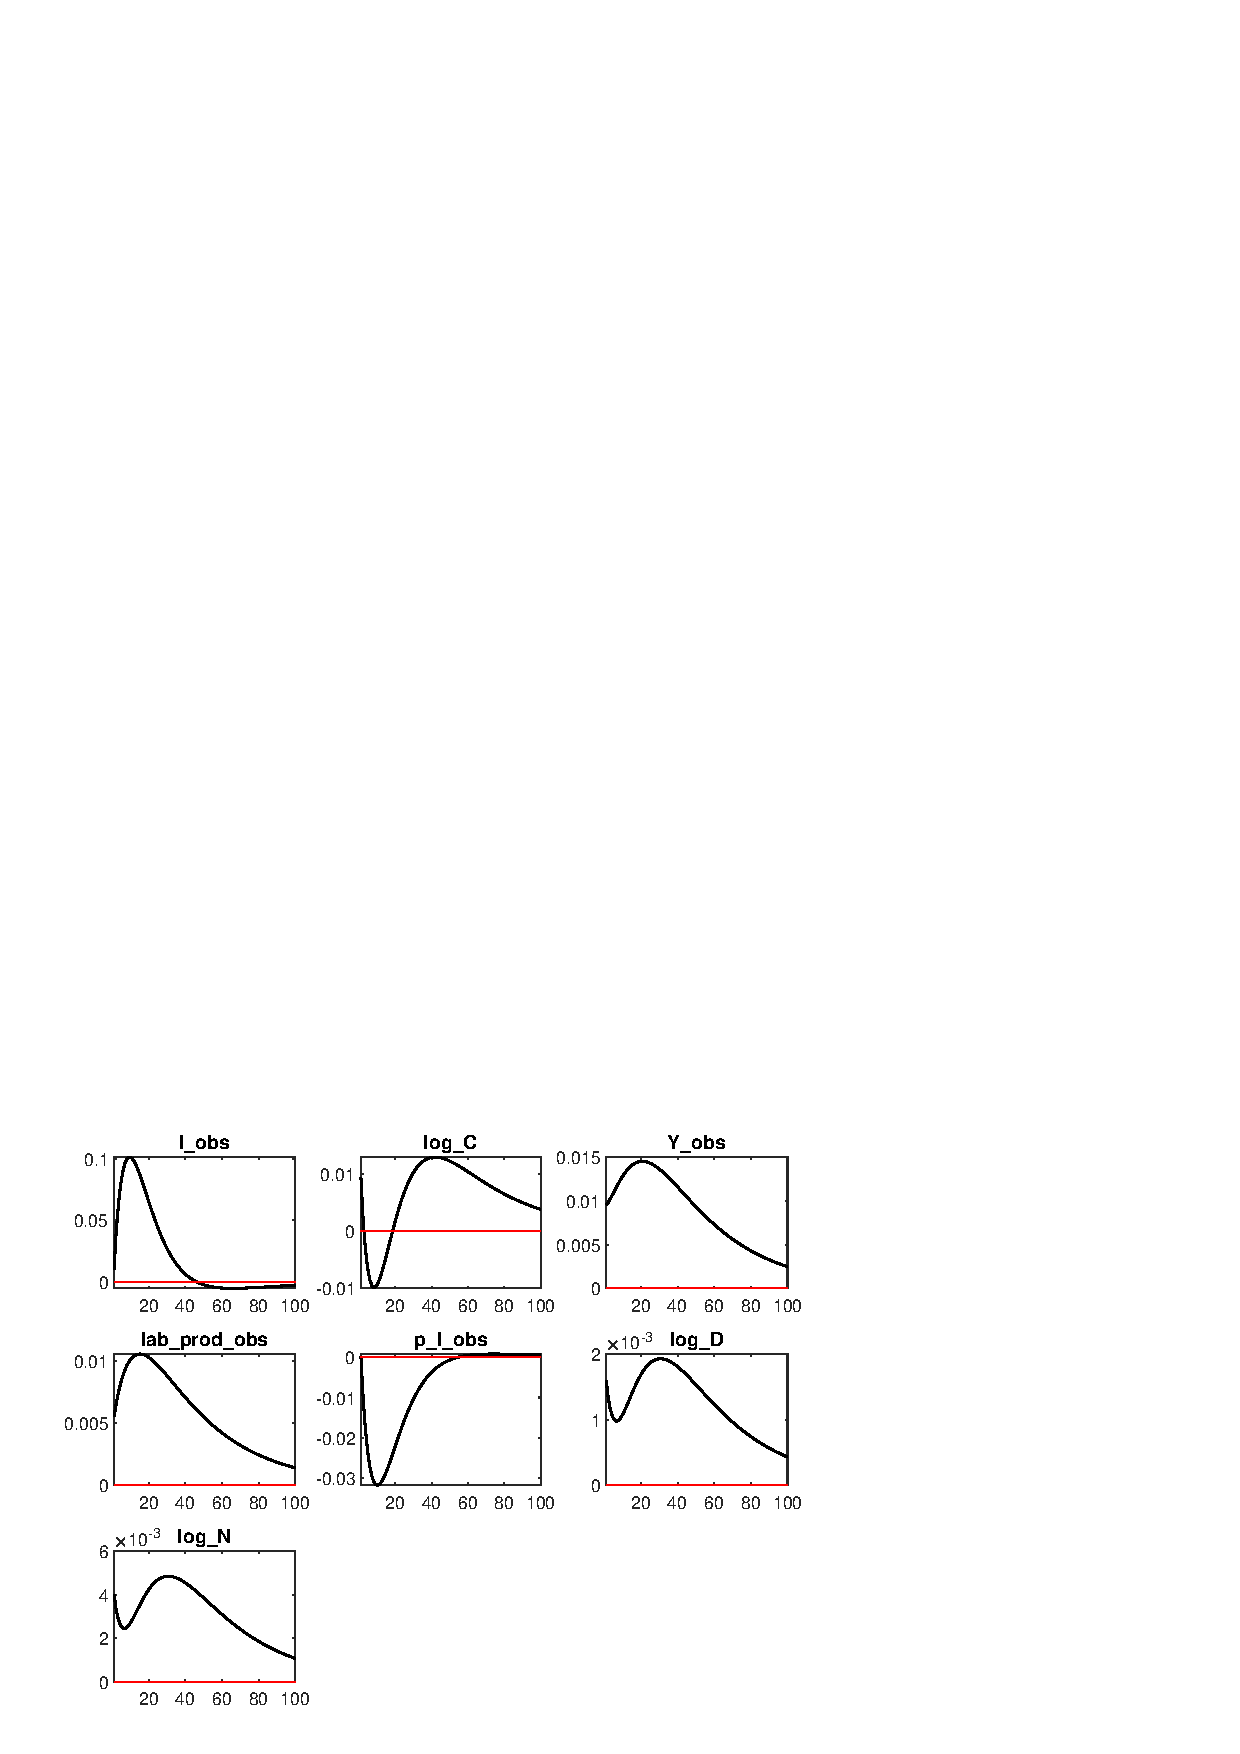
\includegraphics[width=0.80\textwidth]{BRS/graphs/BRS_IRF_e_Z}
\caption{Impulse response functions (orthogonalized shock to ${e_Z}$).}
\label{Fig:IRF:e_Z}
\end{figure}
 
\begin{figure}[H]
\centering 
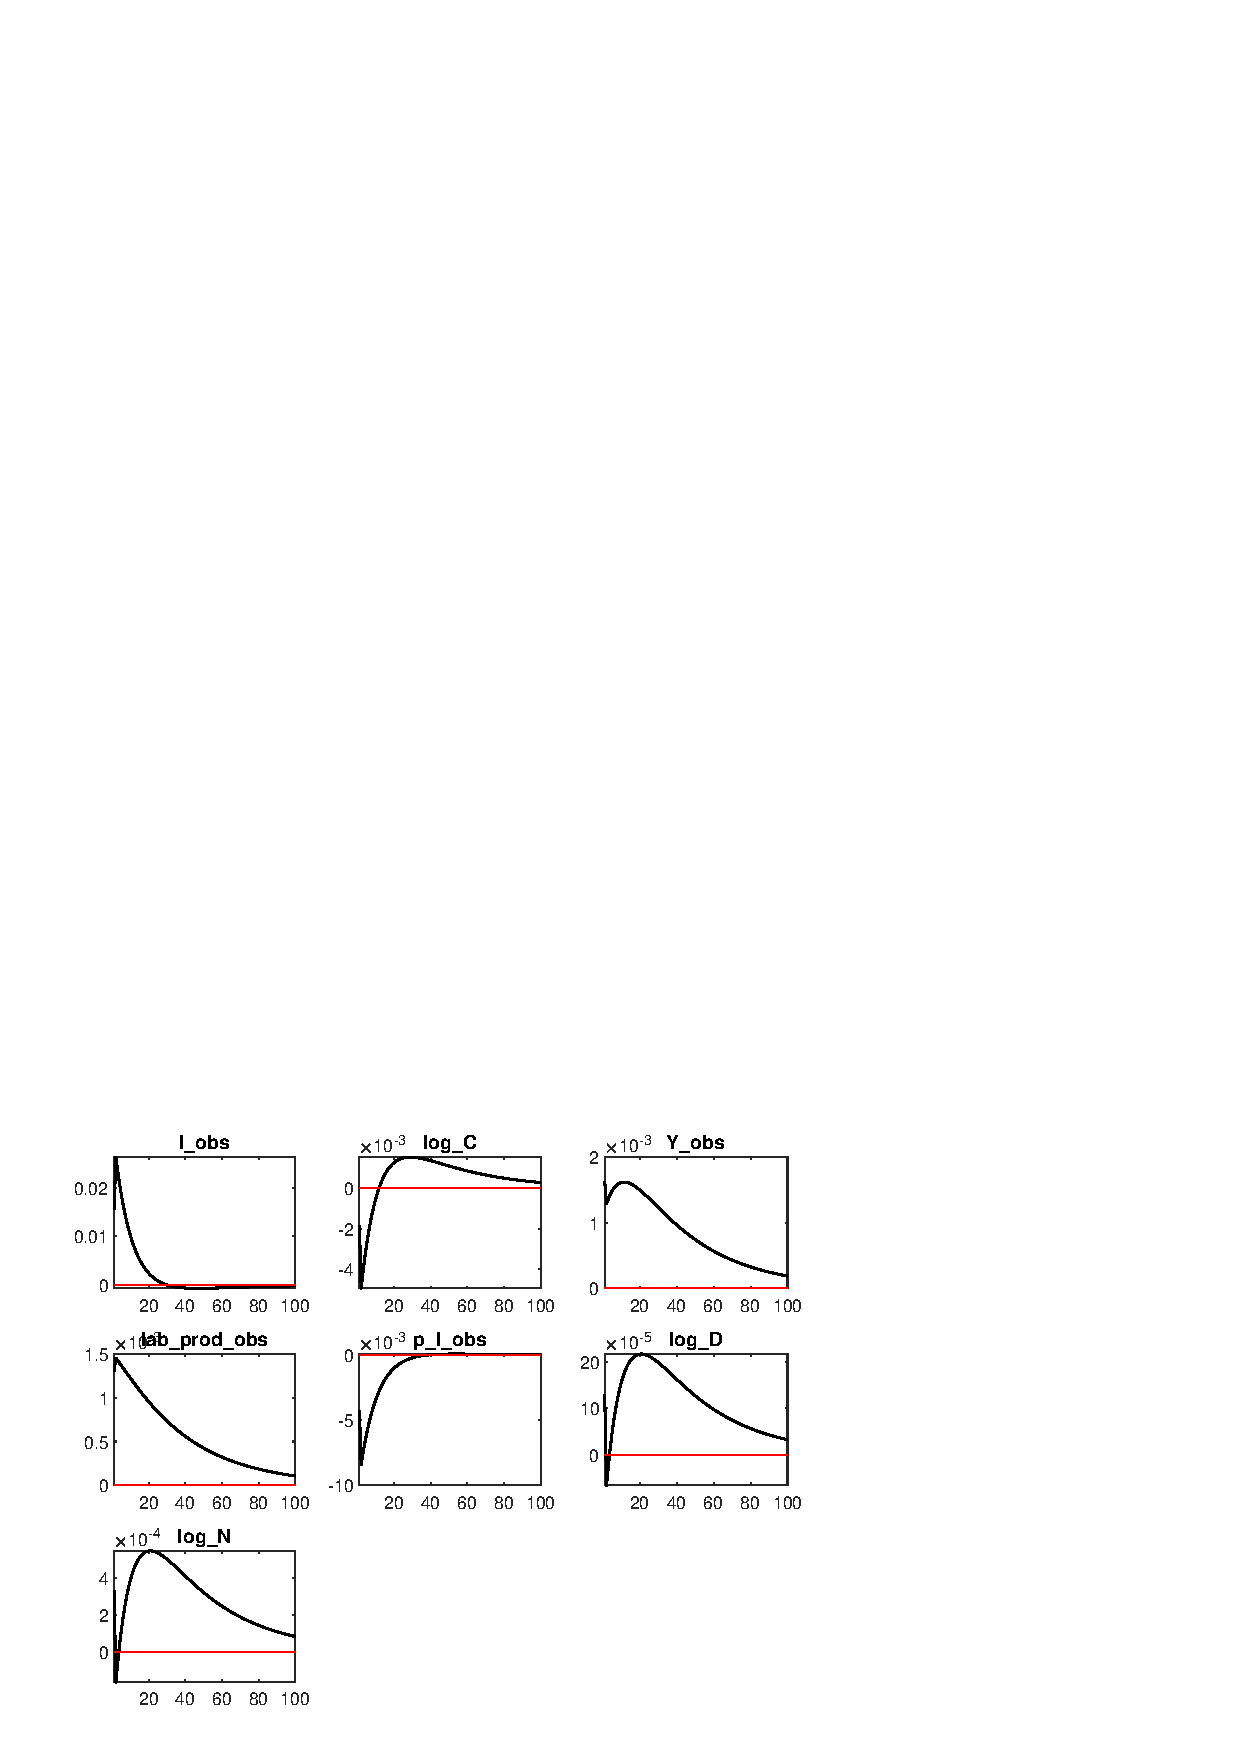
\includegraphics[width=0.80\textwidth]{BRS/graphs/BRS_IRF_e_ZI}
\caption{Impulse response functions (orthogonalized shock to ${e_ZI}$).}
\label{Fig:IRF:e_ZI}
\end{figure}
 
\begin{figure}[H]
\centering 
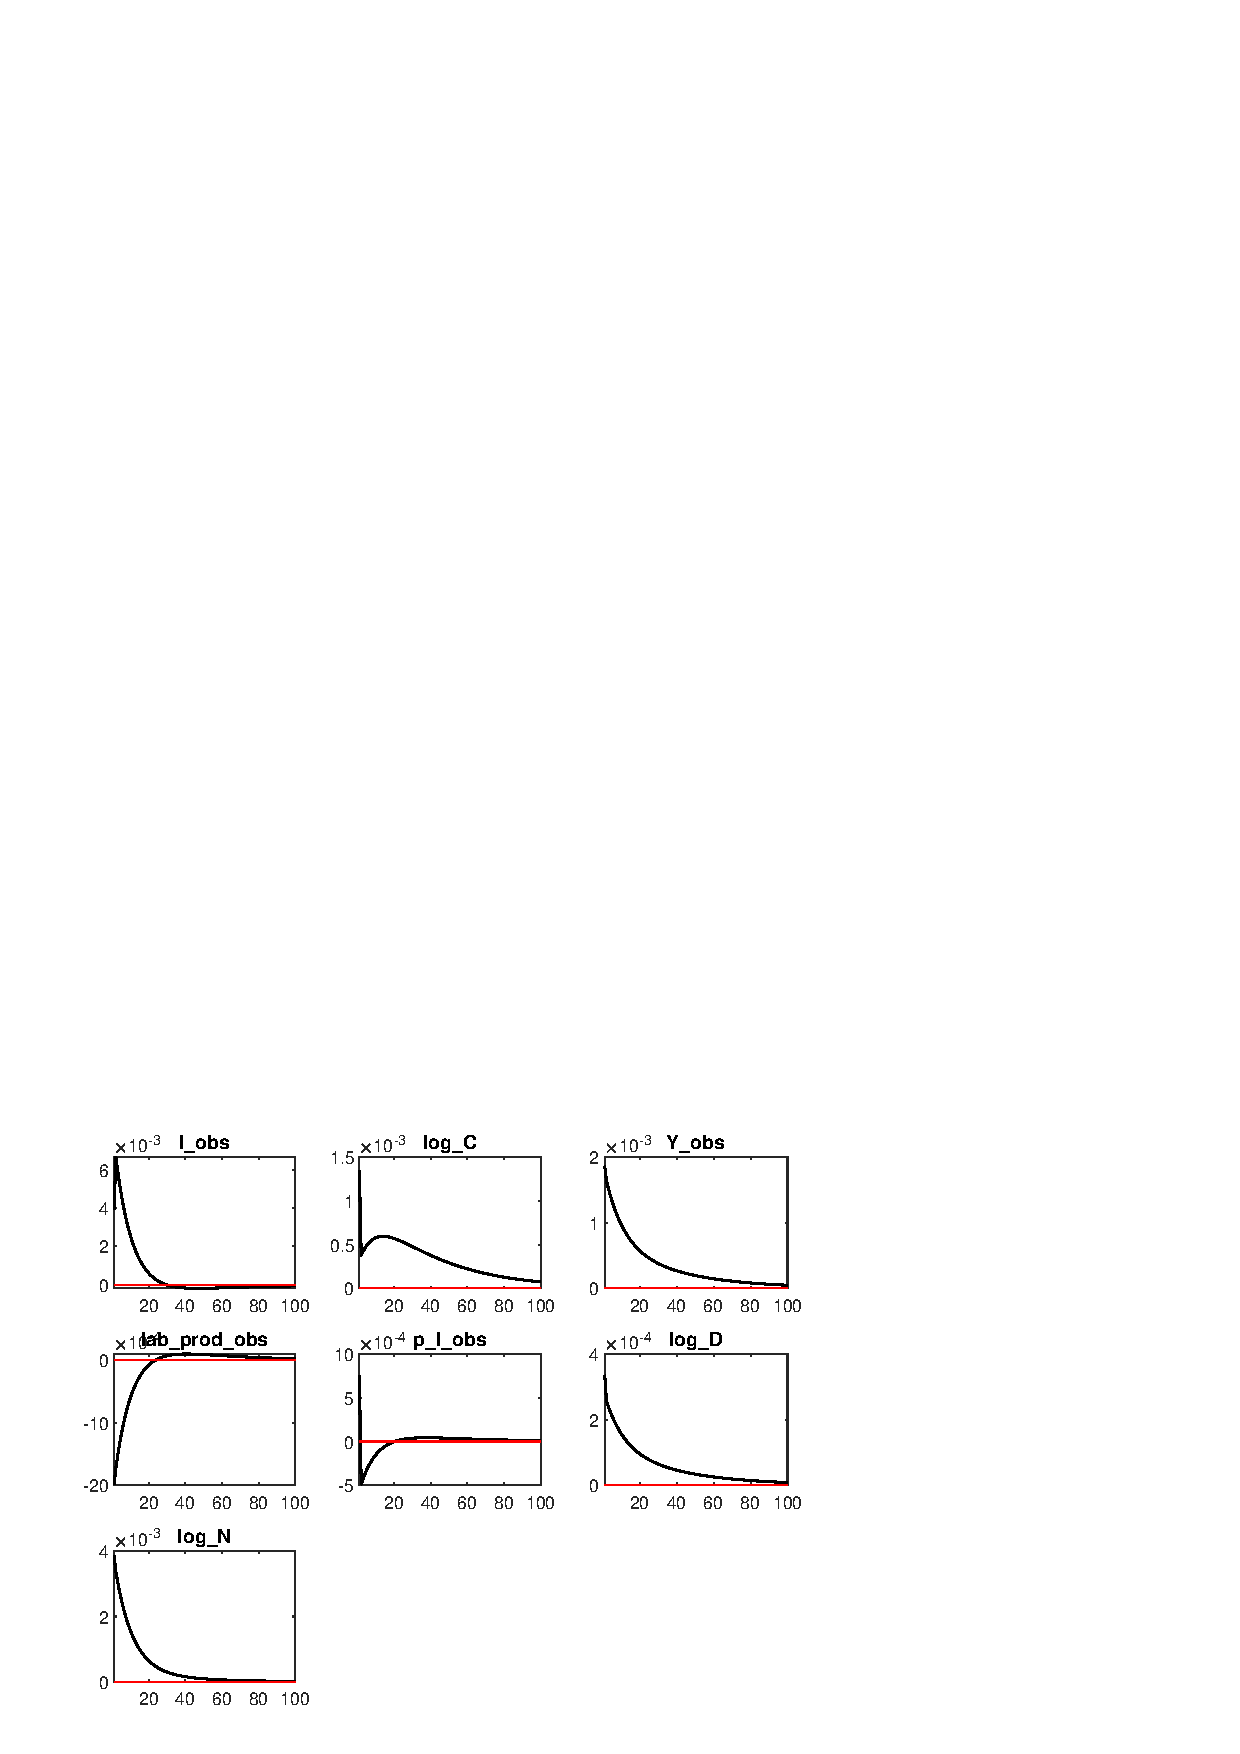
\includegraphics[width=0.80\textwidth]{BRS/graphs/BRS_IRF_e_N}
\caption{Impulse response functions (orthogonalized shock to ${e_N}$).}
\label{Fig:IRF:e_N}
\end{figure}
 
\begin{figure}[H]
\centering 
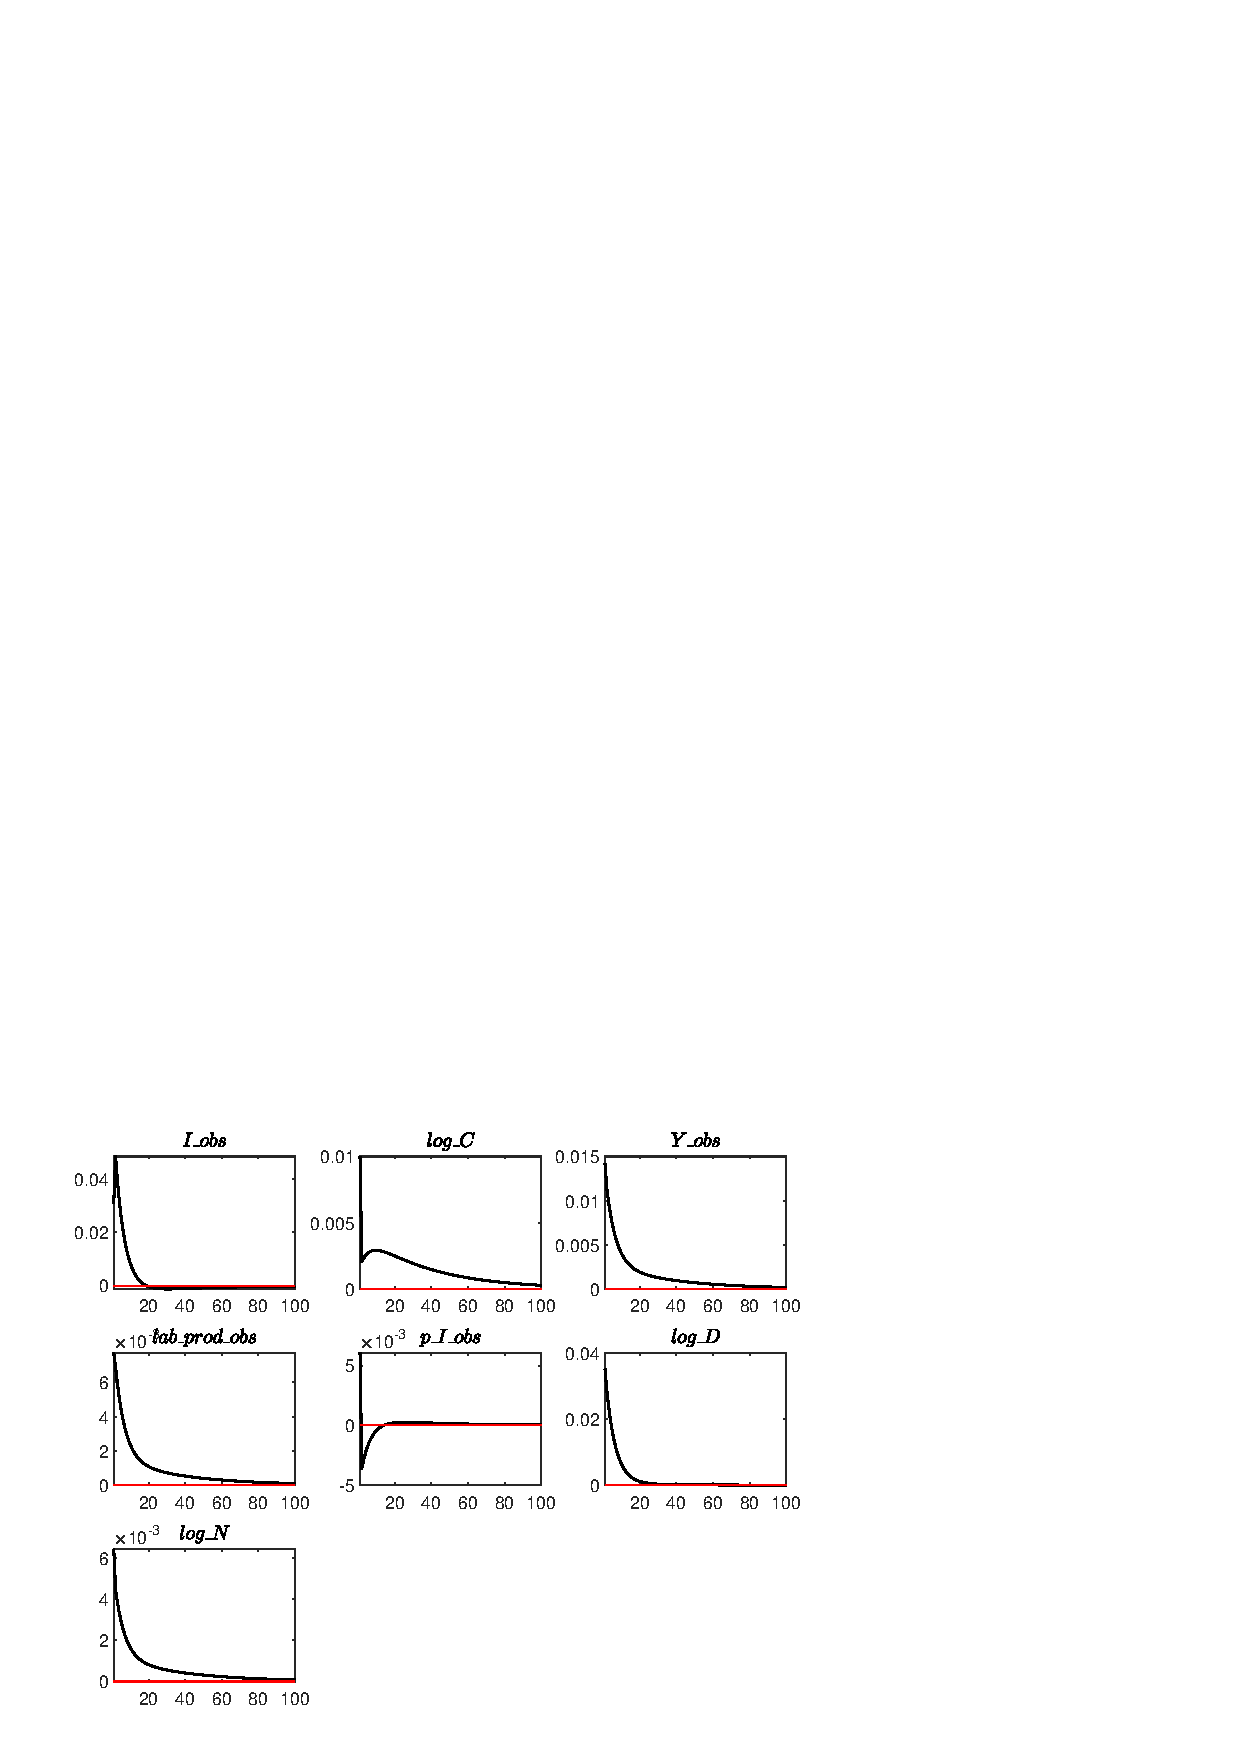
\includegraphics[width=0.80\textwidth]{BRS/graphs/BRS_IRF_e_D}
\caption{Impulse response functions (orthogonalized shock to ${e_D}$).}
\label{Fig:IRF:e_D}
\end{figure}
 
 
% End Of TeX file. 
 
% TeX eps-loader file generated by plot_priors.m (Dynare).
% 23-Jan-2024 12:11:42
 
\begin{figure}[H]
\centering
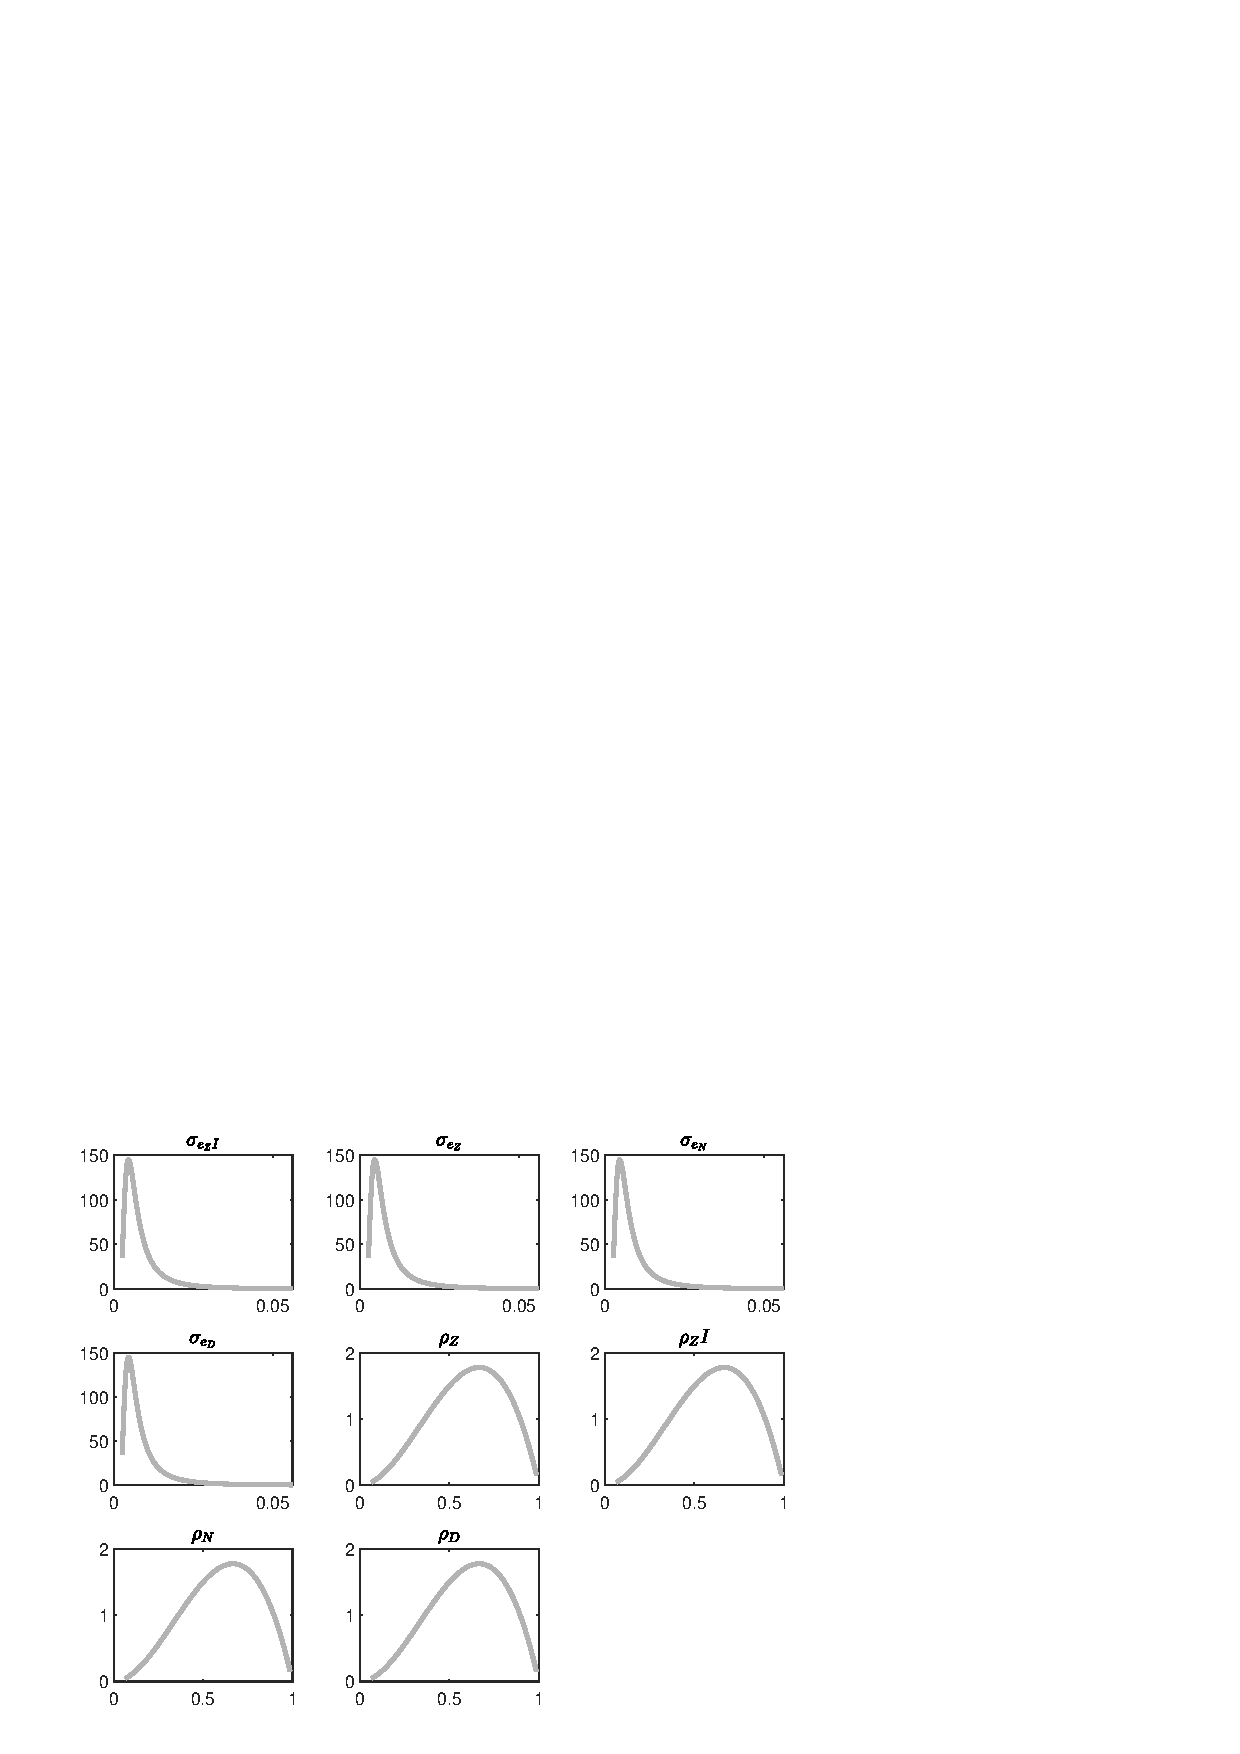
\includegraphics[width=0.80\textwidth]{BRS/graphs/BRS_Priors1}
\caption{Priors.}\label{Fig:Priors:1}
\end{figure}
 
% End of TeX file.
 
% TeX eps-loader file generated by dynare_estimation_1.m (Dynare).
% 23-Jan-2024 16:36:11
 
\begin{figure}[H]
\centering 
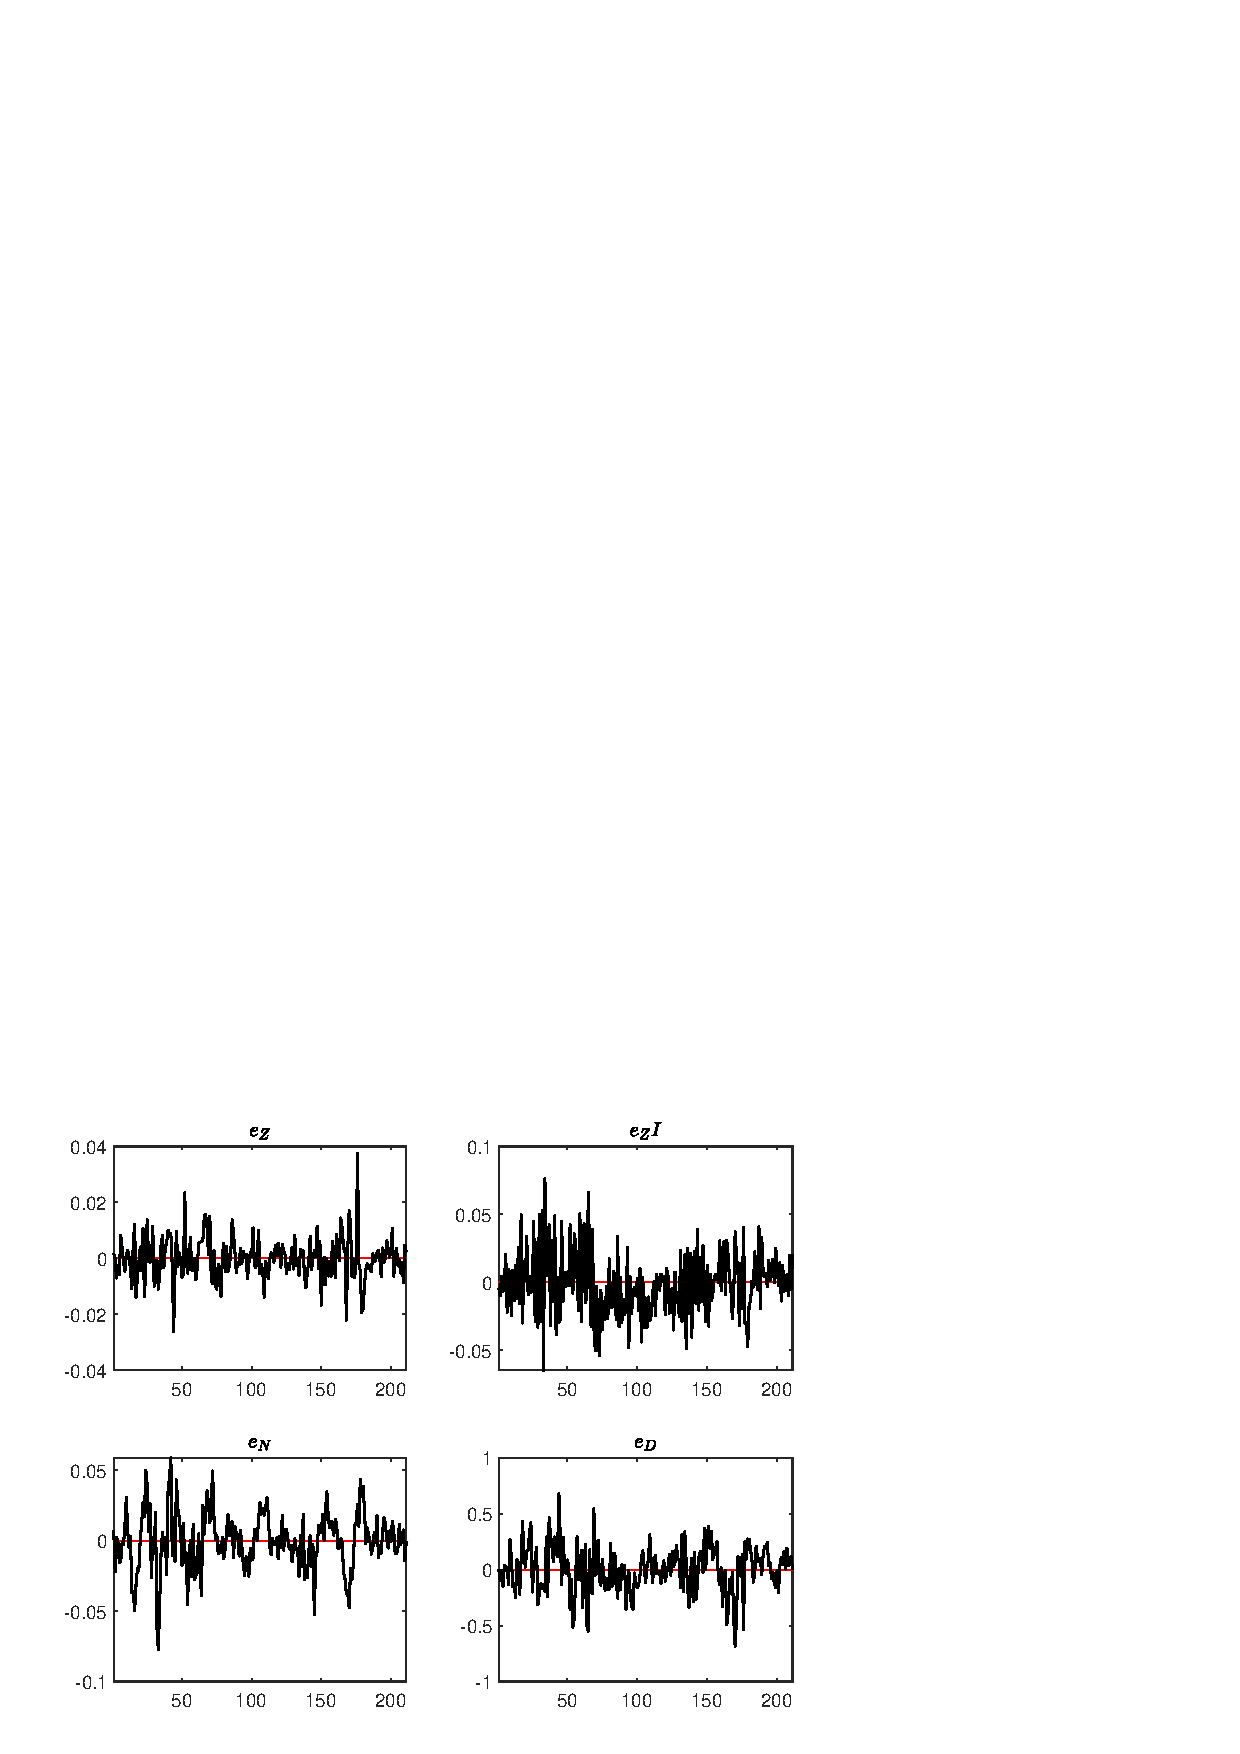
\includegraphics[width=0.80\textwidth]{BRS/graphs/BRS_SmoothedShocks1}
\caption{Smoothed shocks.}\label{Fig:SmoothedShocks:1}
\end{figure}


% End of TeX file.
 
\begin{figure}[H]
\centering
  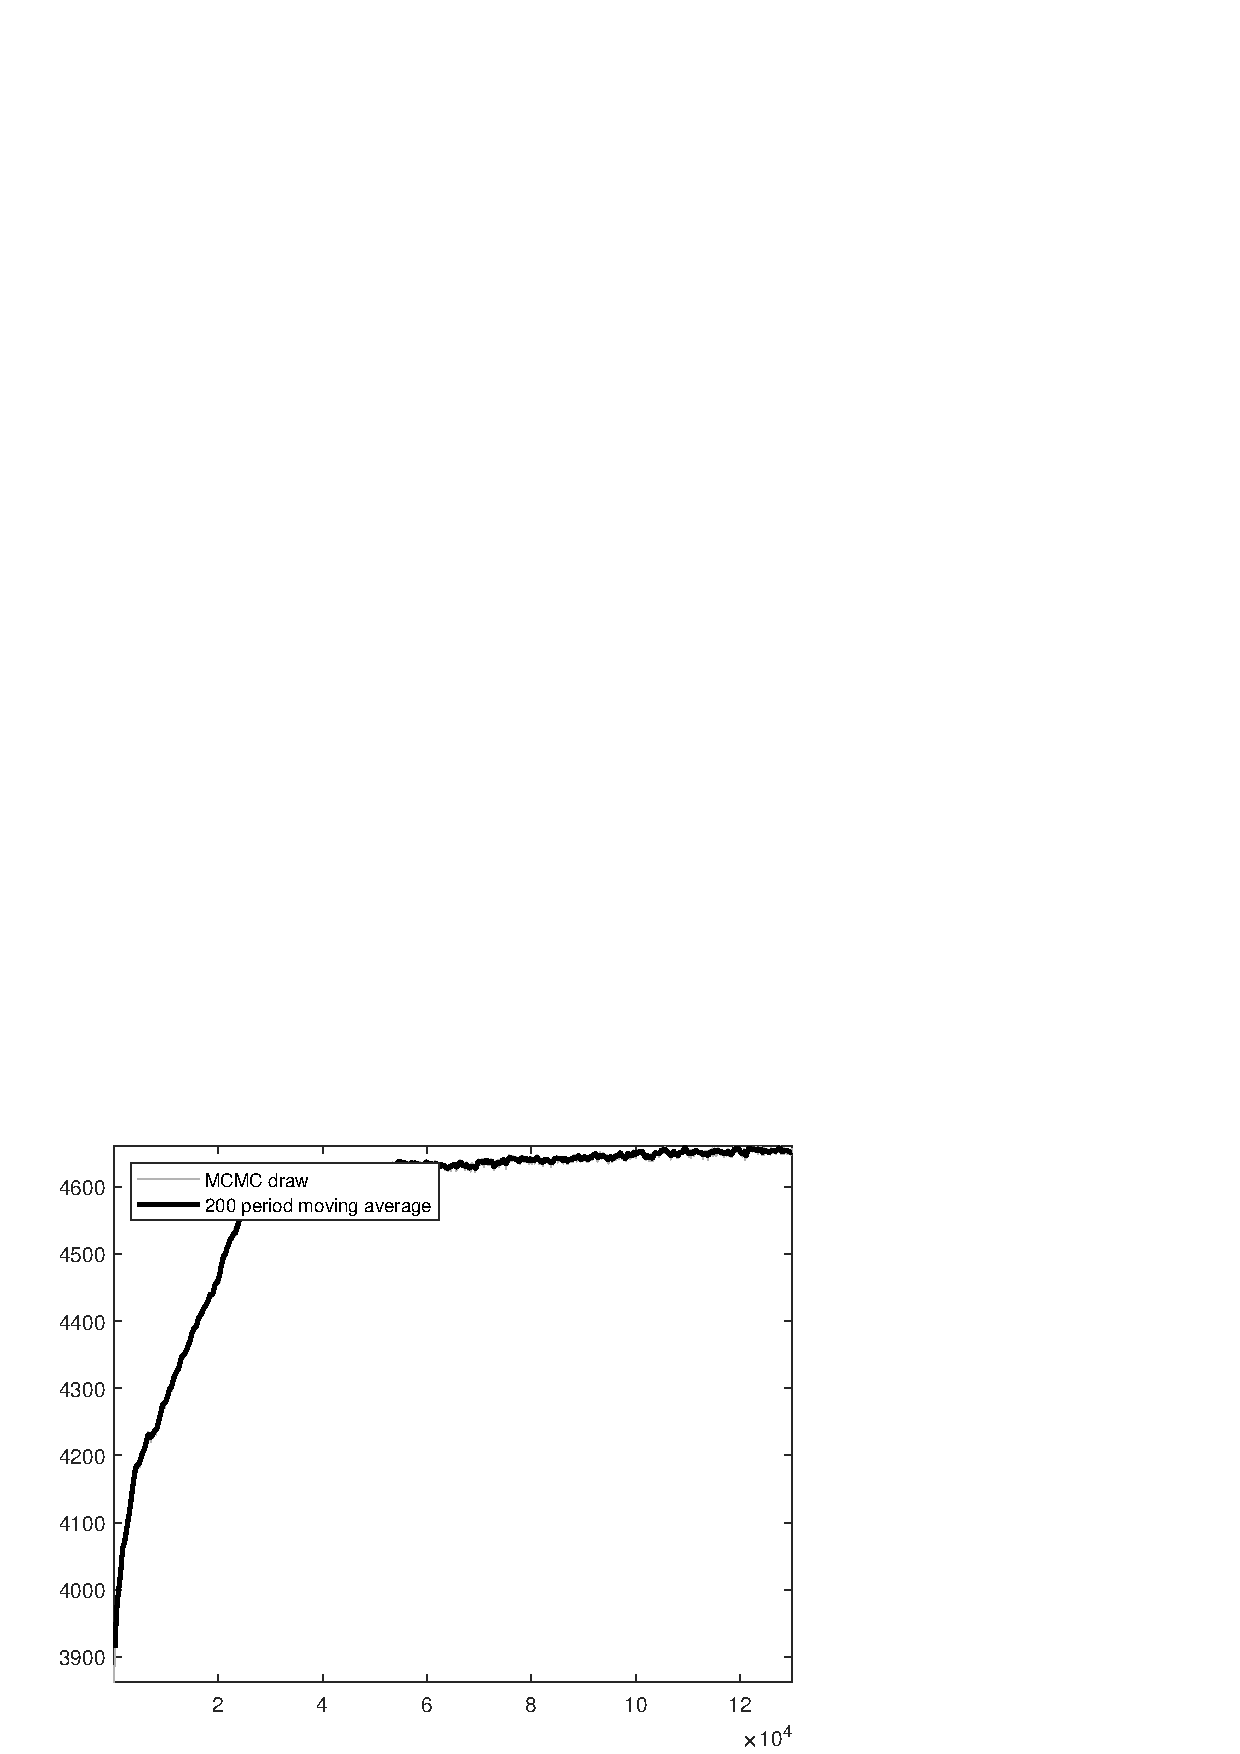
\includegraphics[width=0.8\textwidth]{BRS/graphs/TracePlot_Posterior_blck_1}\\
    \caption{Trace plot for the posterior density (block number 1).}
\end{figure}
 
\begin{figure}[H]
\centering
  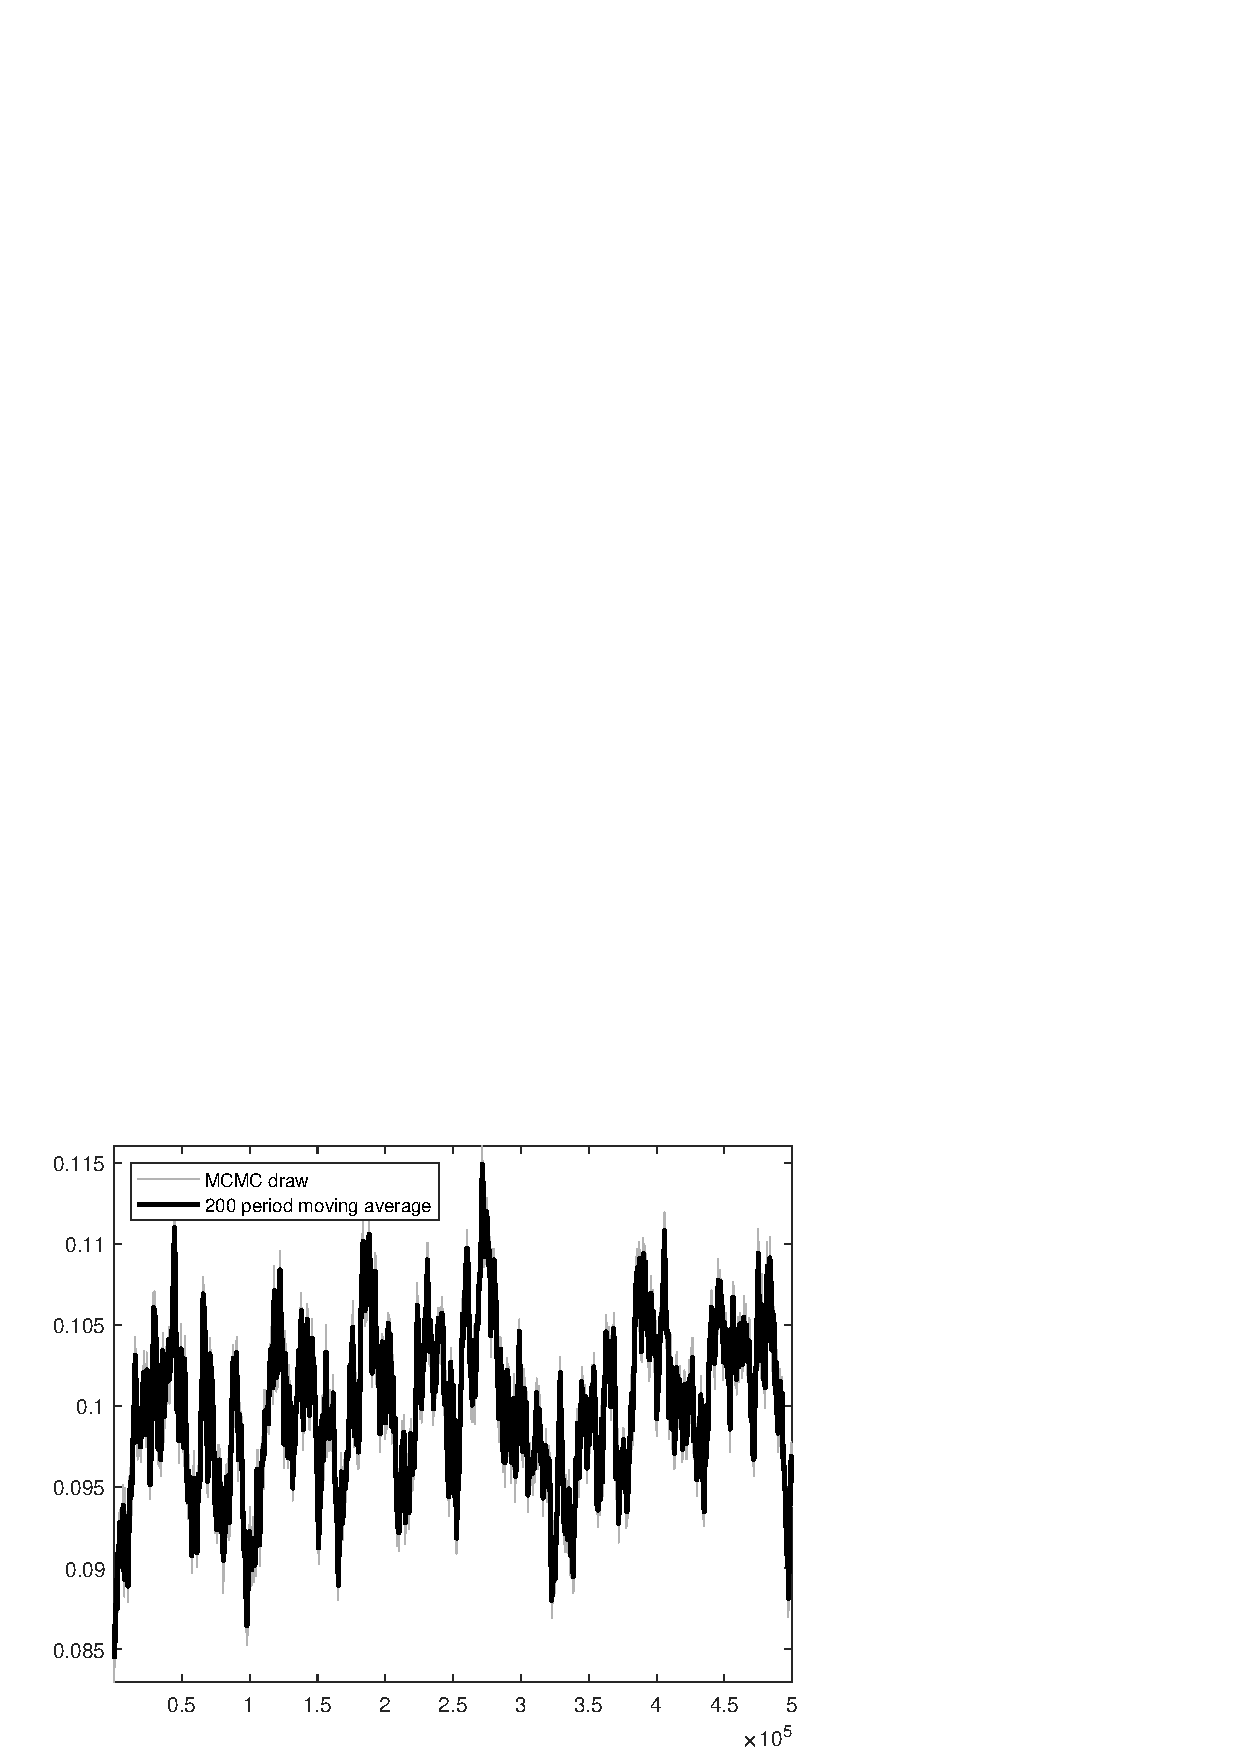
\includegraphics[width=0.8\textwidth]{BRS/graphs/TracePlot_SE_e_D_blck_1}\\
    \caption{Trace plot for the standard deviation of structural shock ${e_D}$ (block number 1).}
\end{figure}
 
\begin{figure}[H]
\centering
  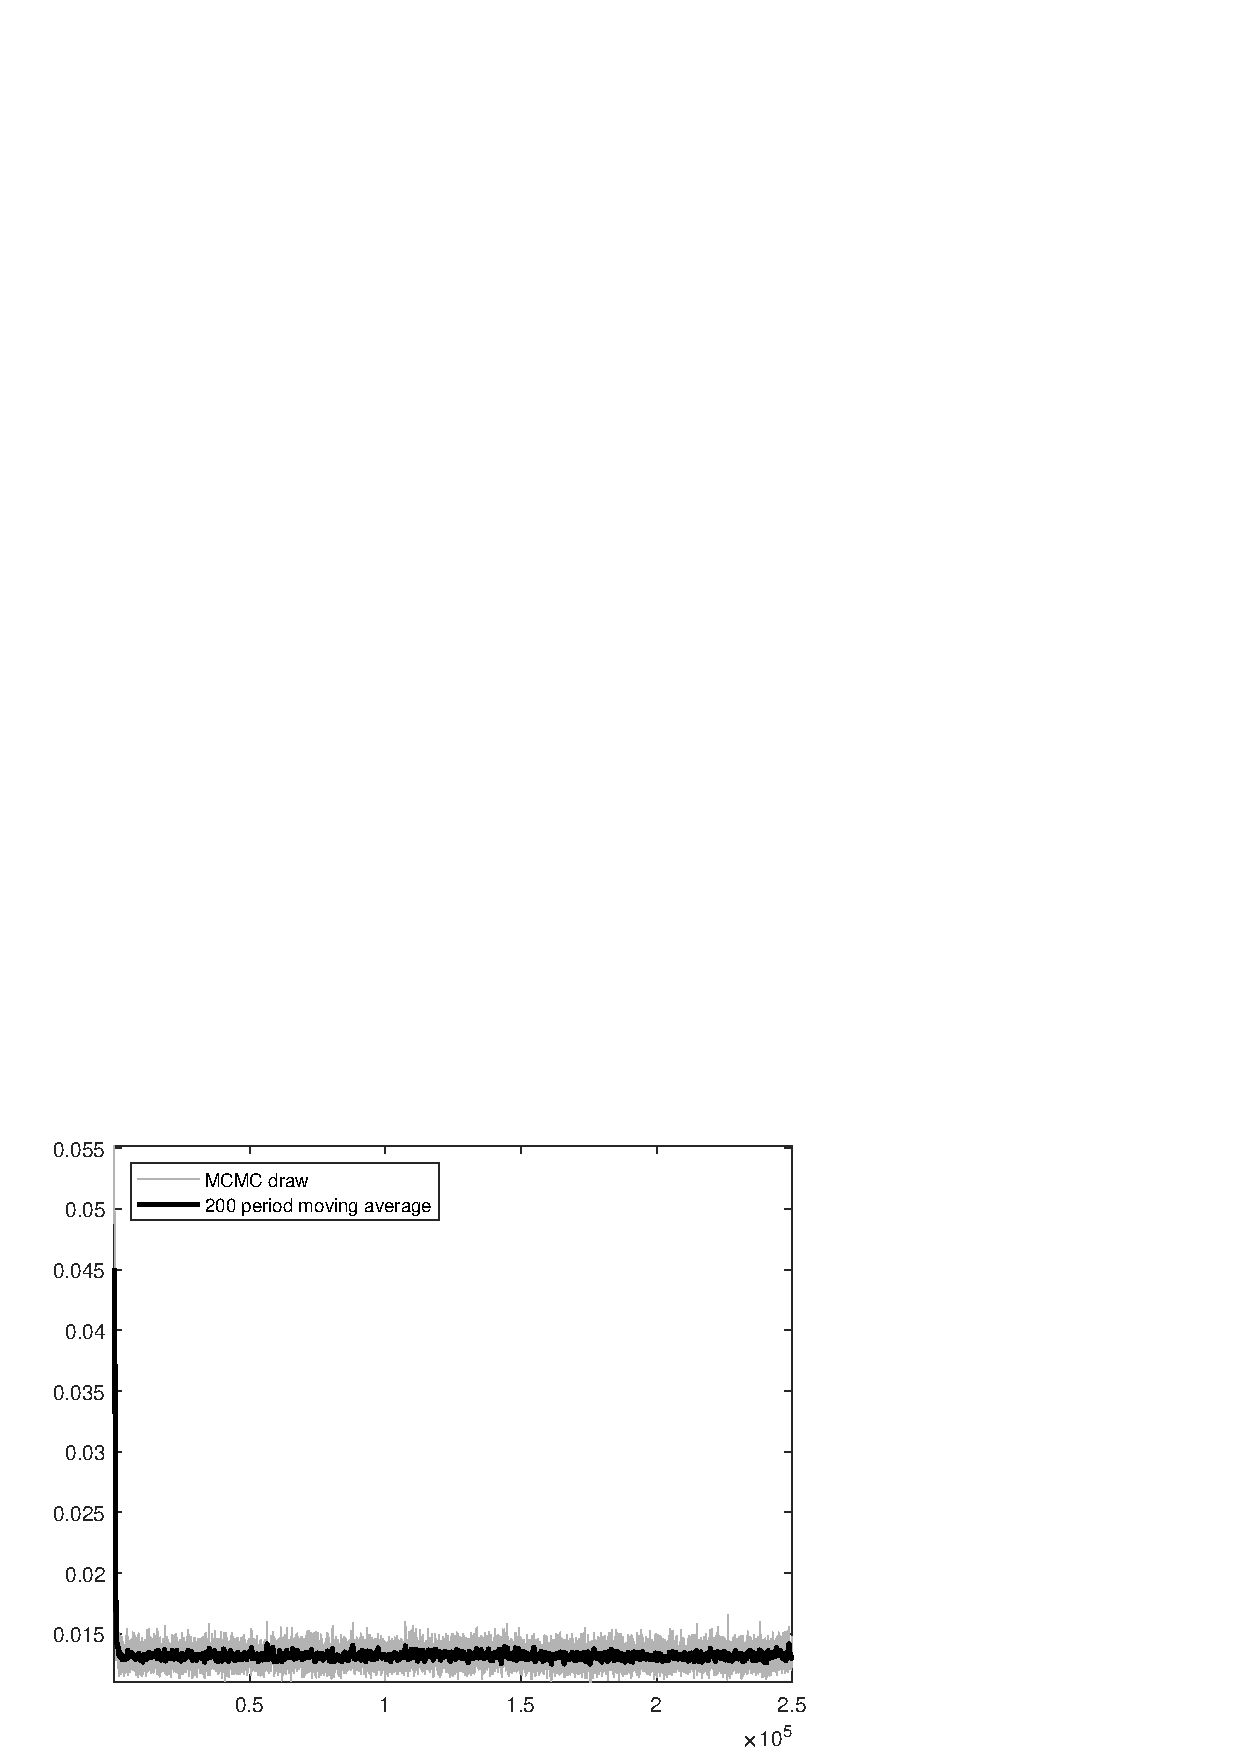
\includegraphics[width=0.8\textwidth]{BRS/graphs/TracePlot_SE_e_N_blck_1}\\
    \caption{Trace plot for the standard deviation of structural shock ${e_N}$ (block number 1).}
\end{figure}
 
\begin{figure}[H]
\centering
  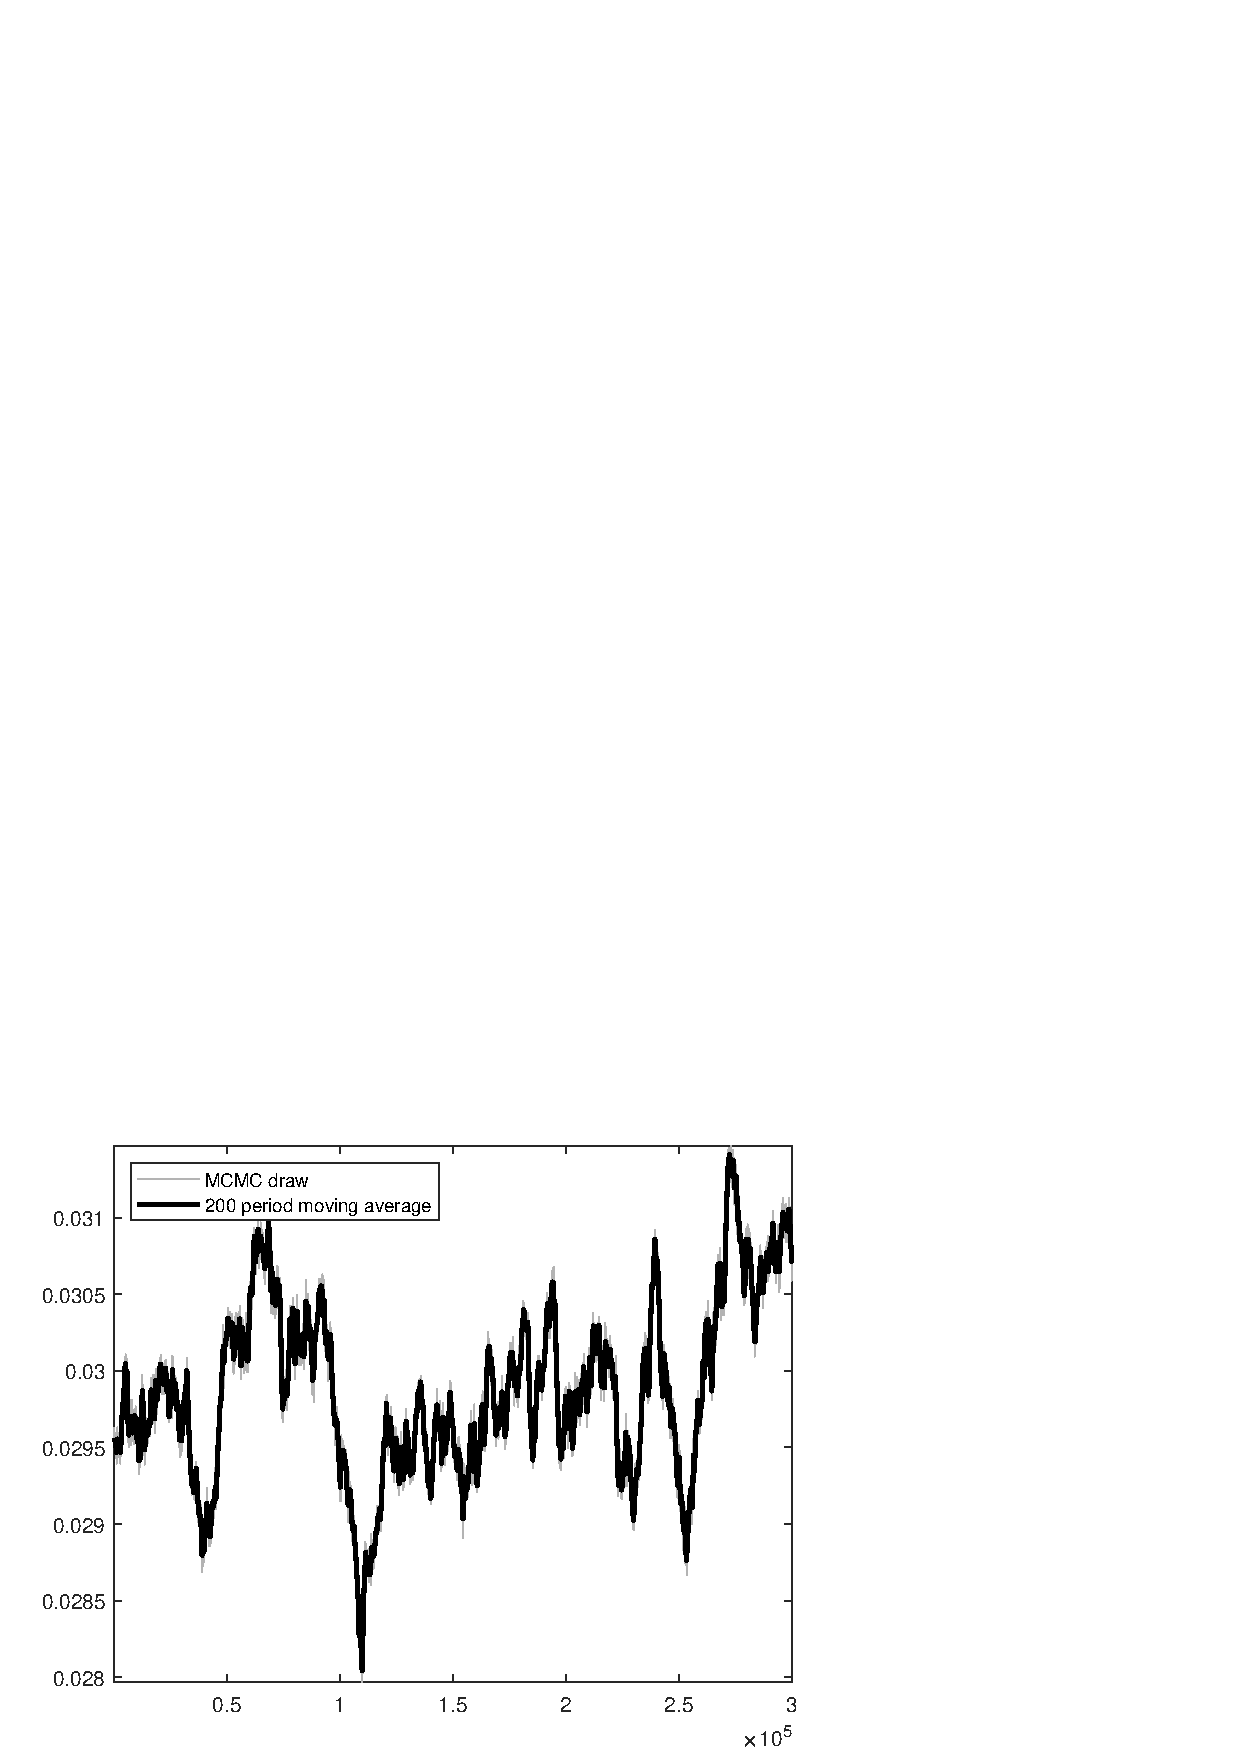
\includegraphics[width=0.8\textwidth]{BRS/graphs/TracePlot_SE_e_ZI_blck_1}\\
    \caption{Trace plot for the standard deviation of structural shock ${e_ZI}$ (block number 1).}
\end{figure}
 
\begin{figure}[H]
\centering
  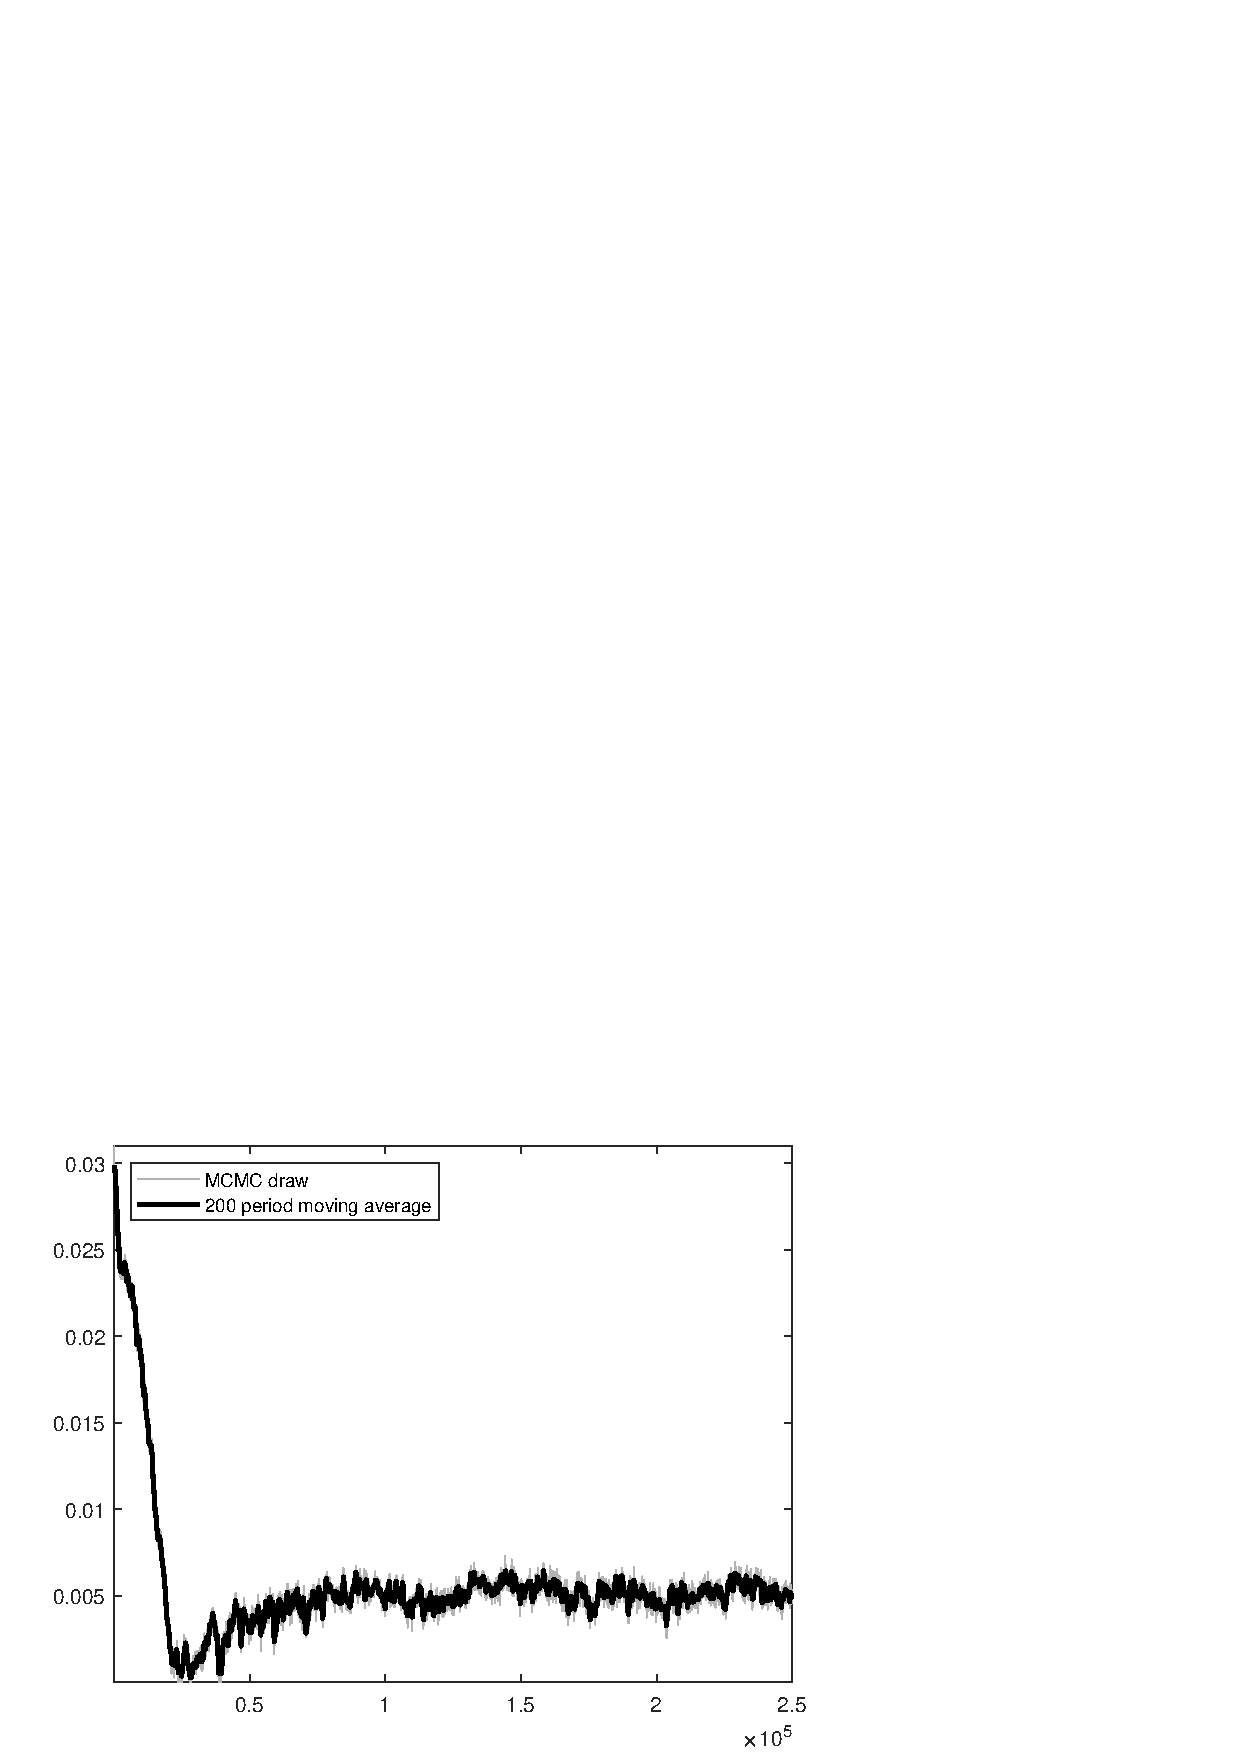
\includegraphics[width=0.8\textwidth]{BRS/graphs/TracePlot_SE_e_Z_blck_1}\\
    \caption{Trace plot for the standard deviation of structural shock ${e_Z}$ (block number 1).}
\end{figure}
 
\begin{figure}[H]
\centering
  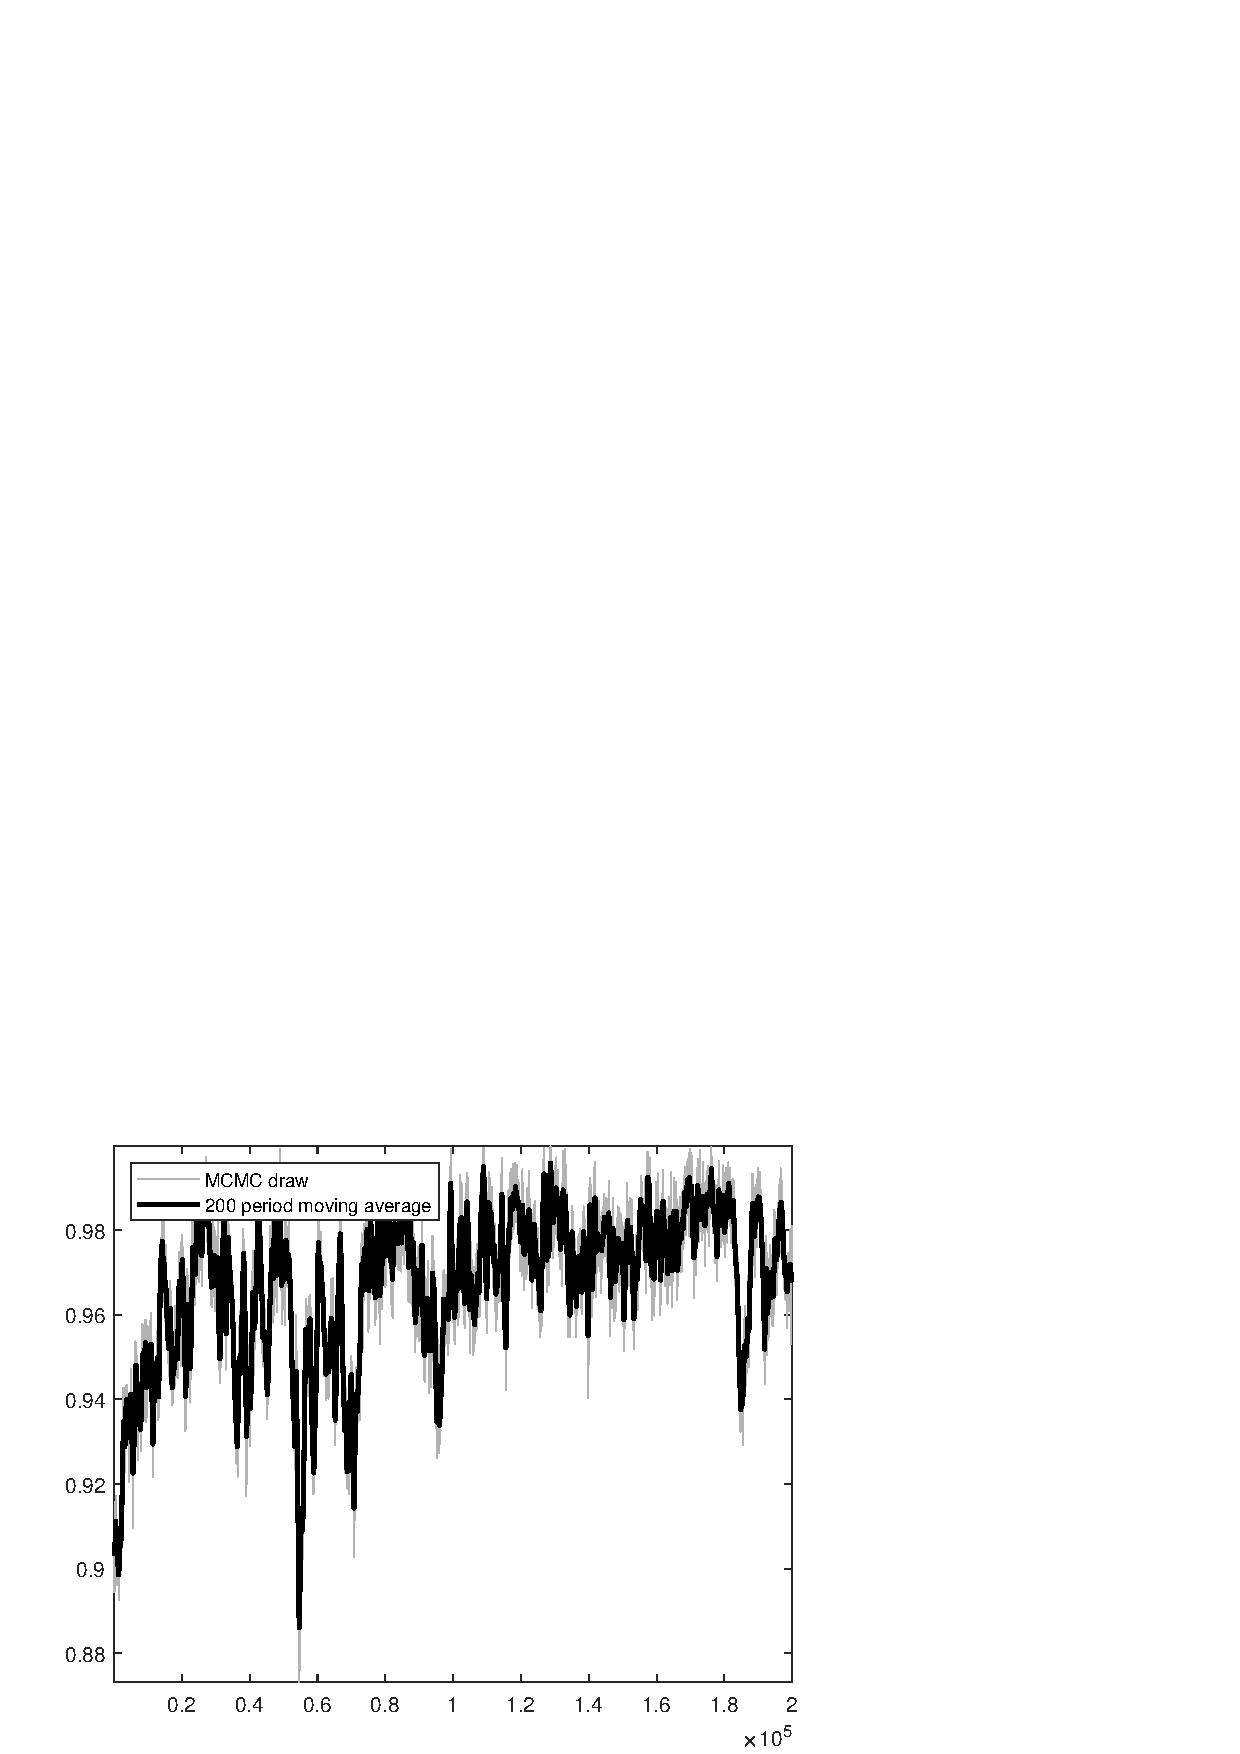
\includegraphics[width=0.8\textwidth]{BRS/graphs/TracePlot_rho_D_blck_1}\\
    \caption{Trace plot for parameter ${\rho_D}$ (block number 1).}
\end{figure}
 
\begin{figure}[H]
\centering
  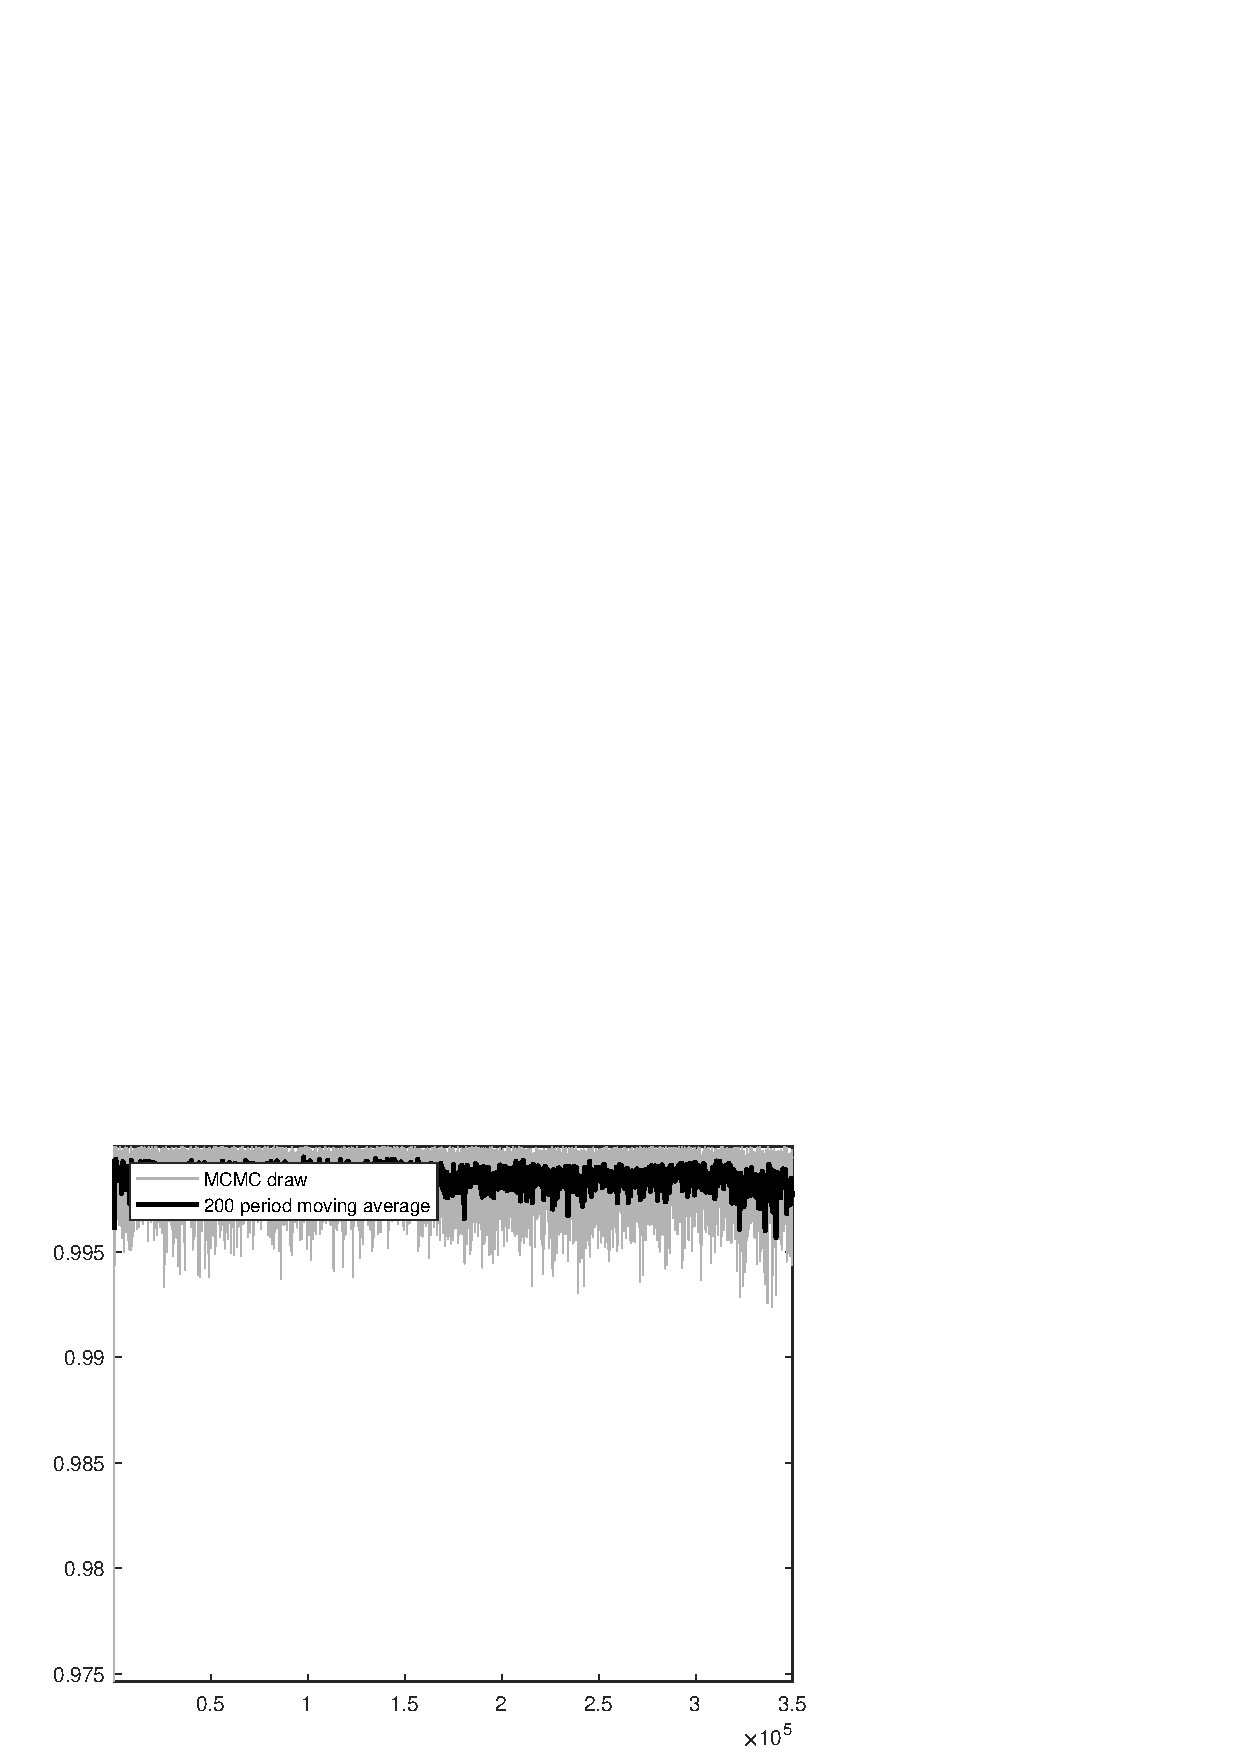
\includegraphics[width=0.8\textwidth]{BRS/graphs/TracePlot_rho_N_blck_1}\\
    \caption{Trace plot for parameter ${\rho_N}$ (block number 1).}
\end{figure}
 
\begin{figure}[H]
\centering
  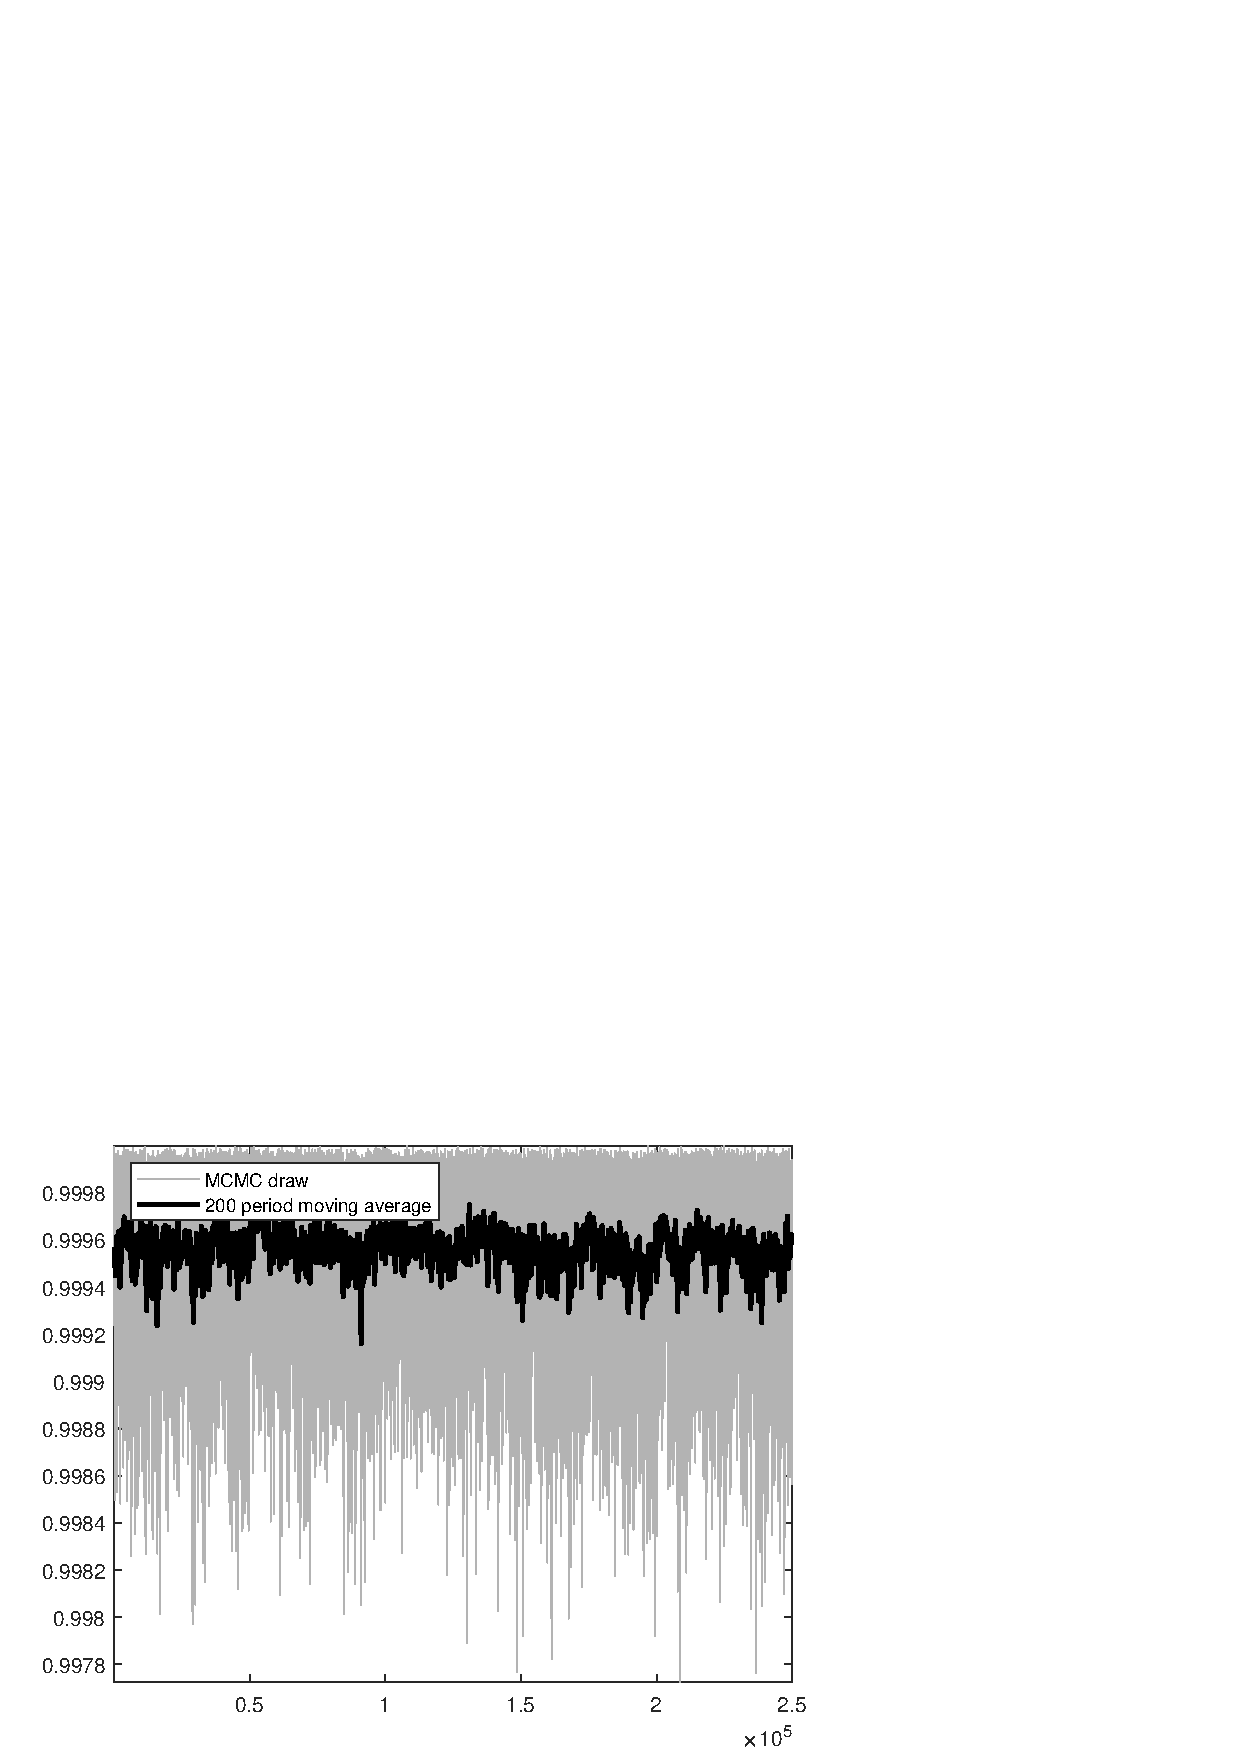
\includegraphics[width=0.8\textwidth]{BRS/graphs/TracePlot_rho_ZI_blck_1}\\
    \caption{Trace plot for parameter ${\rho_ZI}$ (block number 1).}
\end{figure}
 
\begin{figure}[H]
\centering
  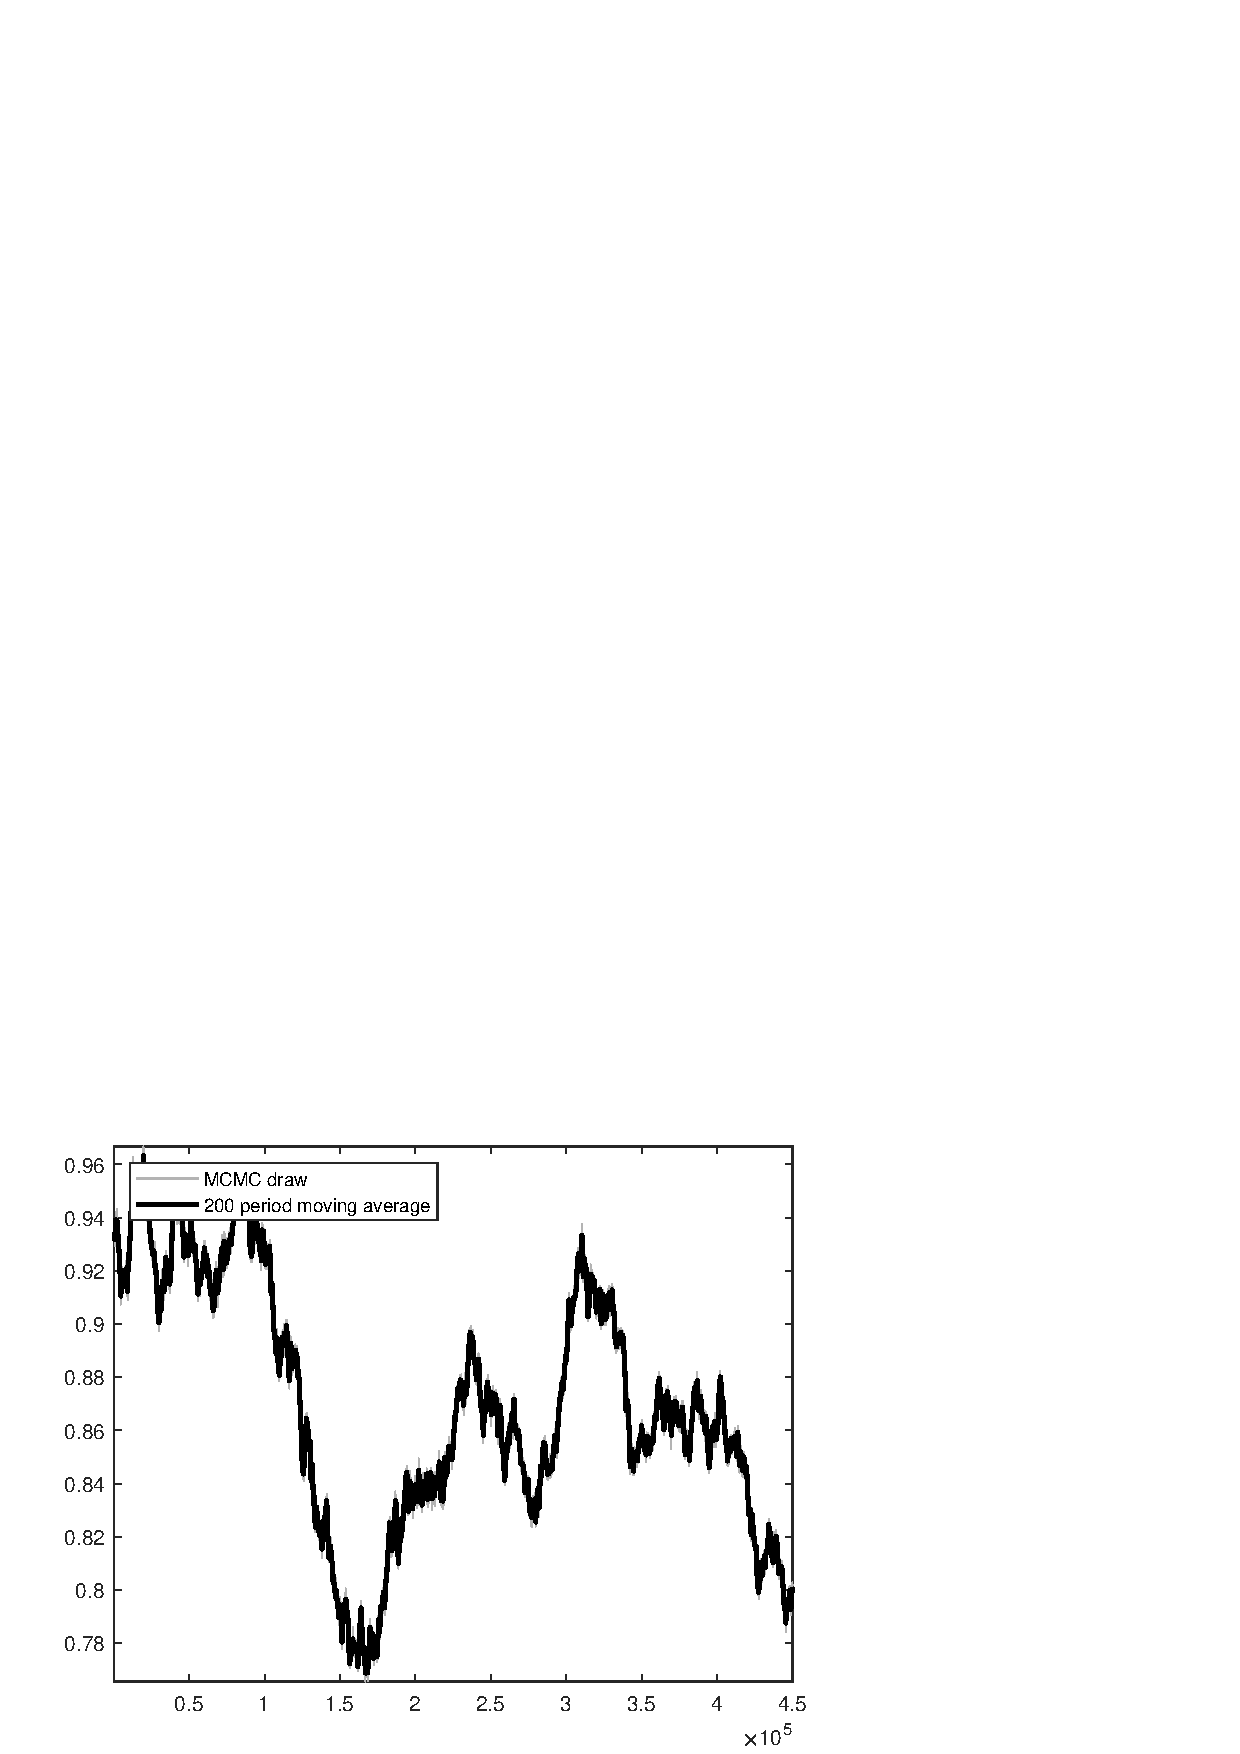
\includegraphics[width=0.8\textwidth]{BRS/graphs/TracePlot_rho_Z_blck_1}\\
    \caption{Trace plot for parameter ${\rho_Z}$ (block number 1).}
\end{figure}
 
\end{document} 
